% Options for packages loaded elsewhere
\PassOptionsToPackage{unicode}{hyperref}
\PassOptionsToPackage{hyphens}{url}
\PassOptionsToPackage{dvipsnames,svgnames,x11names}{xcolor}
%
\documentclass[
  10pt,
]{scrbook}
\usepackage{amsmath,amssymb}
\usepackage{lmodern}
\usepackage{iftex}
\ifPDFTeX
  \usepackage[T1]{fontenc}
  \usepackage[utf8]{inputenc}
  \usepackage{textcomp} % provide euro and other symbols
\else % if luatex or xetex
  \usepackage{unicode-math}
  \defaultfontfeatures{Scale=MatchLowercase}
  \defaultfontfeatures[\rmfamily]{Ligatures=TeX,Scale=1}
\fi
% Use upquote if available, for straight quotes in verbatim environments
\IfFileExists{upquote.sty}{\usepackage{upquote}}{}
\IfFileExists{microtype.sty}{% use microtype if available
  \usepackage[]{microtype}
  \UseMicrotypeSet[protrusion]{basicmath} % disable protrusion for tt fonts
}{}
\makeatletter
\@ifundefined{KOMAClassName}{% if non-KOMA class
  \IfFileExists{parskip.sty}{%
    \usepackage{parskip}
  }{% else
    \setlength{\parindent}{0pt}
    \setlength{\parskip}{6pt plus 2pt minus 1pt}}
}{% if KOMA class
  \KOMAoptions{parskip=half}}
\makeatother
\usepackage{xcolor}
\IfFileExists{xurl.sty}{\usepackage{xurl}}{} % add URL line breaks if available
\IfFileExists{bookmark.sty}{\usepackage{bookmark}}{\usepackage{hyperref}}
\hypersetup{
  pdftitle={Modeling Mindsets},
  pdfauthor={Christoph Molnar},
  colorlinks=true,
  linkcolor={Maroon},
  filecolor={Maroon},
  citecolor={Blue},
  urlcolor={Blue},
  pdfcreator={LaTeX via pandoc}}
\urlstyle{same} % disable monospaced font for URLs
\usepackage{longtable,booktabs,array}
\usepackage{calc} % for calculating minipage widths
% Correct order of tables after \paragraph or \subparagraph
\usepackage{etoolbox}
\makeatletter
\patchcmd\longtable{\par}{\if@noskipsec\mbox{}\fi\par}{}{}
\makeatother
% Allow footnotes in longtable head/foot
\IfFileExists{footnotehyper.sty}{\usepackage{footnotehyper}}{\usepackage{footnote}}
\makesavenoteenv{longtable}
\usepackage{graphicx}
\makeatletter
\def\maxwidth{\ifdim\Gin@nat@width>\linewidth\linewidth\else\Gin@nat@width\fi}
\def\maxheight{\ifdim\Gin@nat@height>\textheight\textheight\else\Gin@nat@height\fi}
\makeatother
% Scale images if necessary, so that they will not overflow the page
% margins by default, and it is still possible to overwrite the defaults
% using explicit options in \includegraphics[width, height, ...]{}
\setkeys{Gin}{width=\maxwidth,height=\maxheight,keepaspectratio}
% Set default figure placement to htbp
\makeatletter
\def\fps@figure{htbp}
\makeatother
\setlength{\emergencystretch}{3em} % prevent overfull lines
\providecommand{\tightlist}{%
  \setlength{\itemsep}{0pt}\setlength{\parskip}{0pt}}
\setcounter{secnumdepth}{5}
\newlength{\cslhangindent}
\setlength{\cslhangindent}{1.5em}
\newlength{\csllabelwidth}
\setlength{\csllabelwidth}{3em}
\newlength{\cslentryspacingunit} % times entry-spacing
\setlength{\cslentryspacingunit}{\parskip}
\newenvironment{CSLReferences}[2] % #1 hanging-ident, #2 entry spacing
 {% don't indent paragraphs
  \setlength{\parindent}{0pt}
  % turn on hanging indent if param 1 is 1
  \ifodd #1
  \let\oldpar\par
  \def\par{\hangindent=\cslhangindent\oldpar}
  \fi
  % set entry spacing
  \setlength{\parskip}{#2\cslentryspacingunit}
 }%
 {}
\usepackage{calc}
\newcommand{\CSLBlock}[1]{#1\hfill\break}
\newcommand{\CSLLeftMargin}[1]{\parbox[t]{\csllabelwidth}{#1}}
\newcommand{\CSLRightInline}[1]{\parbox[t]{\linewidth - \csllabelwidth}{#1}\break}
\newcommand{\CSLIndent}[1]{\hspace{\cslhangindent}#1}
% Geometry
\usepackage[paperwidth=18.9cm, paperheight=24.61cm, inner=30mm, outer=17mm, top=30mm, bottom=24mm]{geometry}


% Decide for a font
%\usepackage{Alegreya}
%\usepackage[scale=.7]{sourcecodepro}


% Make stuff less floaty
\renewcommand{\textfraction}{0.05}
\renewcommand{\topfraction}{0.8}
\renewcommand{\bottomfraction}{0.8}
\renewcommand{\floatpagefraction}{0.75}

% For proofreading: Big margin on the right and 2x linespace
%\linespread{2}
%\geometry{
%  a4paper,
%    total={189mm,246mm},
%  left=20mm,
%  top=20mm,
%  right=70mm,
%  asymmetric
%}

% Header and footer configuration
\usepackage[automark,headsepline]{scrlayer-scrpage}
% Use scrpage2 instead of scrlayer-scrpage if you want to nicer chapter boxes, see main/main.tex. --- WILL NOT WORK WITH TEXLIVE 2019! ----
%\usepackage[automark,headsepline]{scrpage2}
\pagestyle{scrheadings}
\ihead[\headmark]{\headmark}\ohead{\pagemark}
% alternating chapter / section titles at the top of the page
\automark[section]{chapter}
% Make heading of each page italics and small capitals.
\renewcommand*{\headfont}{\itshape\scshape}
% Name of the chapter (\chapapp), number of the chapter (\thechapter) and no period (\autodot)
\renewcommand*{\chaptermarkformat}{\chapapp~\thechapter\autodot\enskip}
% Removes page numbers from bottom
\ofoot{}


% Turns href urls into foodnotes
\let\oldhref\href
\renewcommand{\href}[2]{#2\footnote{\url{#1}}}

% Create index
\usepackage{makeidx}
\makeindex

% Pages for publishing, like empty pages
\frontmatter
\ifLuaTeX
  \usepackage{selnolig}  % disable illegal ligatures
\fi

\title{Modeling Mindsets}
\usepackage{etoolbox}
\makeatletter
\providecommand{\subtitle}[1]{% add subtitle to \maketitle
  \apptocmd{\@title}{\par {\large #1 \par}}{}{}
}
\makeatother
\subtitle{The Many Cultures of Learning From Data}
\author{Christoph Molnar}
\date{2022-06-24}

\begin{document}
\maketitle

%\cleardoublepage\newpage\thispagestyle{empty}\null
%\cleardoublepage\newpage\thispagestyle{empty}\null
%\cleardoublepage\newpage
\thispagestyle{empty}
%\begin{center}
%\includegraphics{images/dedication.pdf}
%\end{center}

%\setlength{\abovedisplayskip}{-5pt}
%\setlength{\abovedisplayshortskip}{-5pt}


% =========================================================================
% Title page with cover
% =========================================================================

\iffalse
\thispagestyle{empty}

\vspace{3cm}
  \begin{center}
    {
	\bfseries \sffamily \Huge Modeling Mindsets for Data Scientists \par
	\bfseries \LARGE The Many Cultures of Learning From Data \par
~\\
	~\\
	\bfseries \small Published by Christoph Molnar, Munich\par
      }
  \end{center}


\newpage
\fi
% =========================================================================
% Page with publishing details
% =========================================================================



\thispagestyle{empty}
\begin{center}
  {
  \bfseries \sffamily \LARGE Modeling Mindsets for Data Scientists \par
  \bfseries \small The Many Cultures of Learning From Data  \par
}

\copyright~2022 \textit{Christoph Molnar}, Germany, Munich\\
\url{christophmolnar.com}

For more information about permission to reproduce selections from this book, write to \url{christoph.molnar.ai@gmail.com}.

	\the\year, First Edition

% Impression line, indicating number and year of current printing
% International Standard Book Number (ISBN)
% International Standard Serial Number (ISSN), if applicable
\ifxetex
	\textsc{} 
\fi


\includegraphics{images/by-nc-sa.png}

This book is licensed under the Creative Commons Attribution-NonCommercial-ShareAlike 4.0 International License.
% For translations, indication of original-language title, publisher, and copyright, acknowledgments, permissions, and other credits, including acknowledgment of grants, if applicable and space permitting
  
  Christoph Molnar,
  c/o Mucbook Clubhouse,
  Westendstraße 78,
  80339 München, Germany

\end{center}

% =========================================================================
% Dedication / Empty page before outline
% =========================================================================
\newpage
\thispagestyle{empty}
\mbox{}
\newpage








{
\hypersetup{linkcolor=}
\setcounter{tocdepth}{1}
\tableofcontents
}
\hypertarget{summary}{%
\chapter*{Summary}\label{summary}}


We use data to advance science, make businesses more profitable, automate annoying tasks, and develop smart products.
But there is a middleman between data and its usefulness: the \textbf{model}.
The model represents a simplified aspect of the world; it's the glue that connects data and world.

Statistics versus machine learning, frequentist versus Bayesian inference, causation or association, \ldots{}
There are many mindsets to consider for building models from data.
Each of these modeling mindsets has its own assumptions, strengths, and limitations.

\textbf{The best modelers, researchers, and data scientists don't stubbornly stick to just one mindset}.
The best modelers mix and match the mindsets.

It can take years to truly grasp a new mindset.
Most books and courses jump right into math and methods instead of discussing the fundamental mindset.
But learning a new mindset doesn't have to be this difficult.
\textbf{The Modeling Mindset book introduces many cultures of learning models from data}.
Each of them enhances your own mind and makes you a better modeler:

\begin{itemize}
\tightlist
\item
  Frequentist inference: learning about nature's ``true'' values.
\item
  Bayesian inference: updating your beliefs about the world.
\item
  Supervised machine learning: predicting new data well.
\item
  Causal inference: taking causality seriously.
\item
  Deep learning: embedding the world into a neural network.
\item
  And many more.
\end{itemize}

Modeling Mindsets opens the door to all these different ways of thinking.
The book is packed with \textbf{intuitive explanations and illustrations}.
Quickly get an overview of the strengths and the limitations of each modeling mindset.
Expand your mind when it comes to modeling the world using data.

\hypertarget{what-this-book-is-about}{%
\chapter{What This Book is About}\label{what-this-book-is-about}}

The book is about all the different mindsets that allow you to model the world with data.
Each mindset represents a different perspective on how to see the world through data.
In this book, you will find for each mindset the \textbf{assumptions, central ideas, their relationship to other mindsets, and their strengths and limitations}.
Modeling mindsets is not about history.
Modeling mindsets is a mixture of lightweight methodological introduction and philosophy.
That said, this book is not and \textbf{cannot be a full introduction to each mindset}.
There are entire books about, for example, Bayesian inference, or supervised machine learning.
After reading this book, you will not automatically become a frequentist statistician, or a causal inference expert.
Sorry to disappoint this early in the book.
However, reading Modeling Mindsets can open doors to new ways of thinking about modeling.
But there are other resources to explore what's behind each door -- an online course on machine learning, blog posts about about causal inference, a book about design-based inference, \ldots{}
In each chapter, I refer to \textbf{useful resources to deepen the particular mindset}.

\hypertarget{who-this-book-is-for}{%
\section{Who This Book is For}\label{who-this-book-is-for}}

The book is for data scientists, statisticians, machine learner, quantitative researchers, \ldots{}
In short, for anyone who already has experience with modeling data.
This means you should probably \textbf{know at least one of the mindsets}.
Perhaps, like me, you studied frequentist statistics.
Or you may be a researcher who has learned to use Bayesian inference to analyze your data.
Or maybe you are a self-taught machine learner.

That said, it's crucial that you don't cling to the mindset you already know.
Let go of the rigid assumptions you've learned.
Open your mind to fundamentally new ways of modeling data.

A little math shouldn't scare you either.
But I can promise you that the book is not too heavy on the math side.

\mainmatter

\hypertarget{models}{%
\chapter{Models}\label{models}}

You gaze at the screen.
The screen shows a table with some data.
Based on this data, you are to answer some questions.
These questions could be:

\begin{itemize}
\tightlist
\item
  Which patients might get side effects from a certain drug?
\item
  How do bee hives react to a change in climate?
\item
  Which supermarket products are often out-of-stock?
\end{itemize}

In the data you can see in detail what happened: patients with ID 124 and 22 got acne; 2/3 of bee colonies had trouble during drought in 2018; on that one Tuesday the flour was sold out;
But with data, you can't immediately see general rules and relationships.
Is flour generally in low supply at the beginning of the week?
It would be even better if these rules and relationships applied not only to your specific data sample, but to a more general population of patients/hives/supermarkets.
To move from data to generalizable relationships, we have to simplify the world and make assumptions.
The end result is a model of the world based on data.

A model is a simplified representation of some aspect of the world.
For example, how bee colonies depend on climate.
With a model we can answer questions and make predictions that we couldn't with the raw data.

In this book, we talk about certain types of models:
Models must be computational or mathematical models.
This excludes, for example, physical models, like the tiny houses that architects build.
The second restriction: The models are learned from data.
This excludes ``designed'' models such cellular automata.

There is no philosophical consensus on what makes a model.
For our purpose, let's say that \textbf{a mathematical model consists of three ingredients: variables, relations and parameters}.
A mathematical model contains mathematical structures that represent \emph{variables} and put them in \emph{relation} (Figure \ref{fig:model}).\textsuperscript{\protect\hyperlink{ref-weisberg2012simulation}{1}}
The relations are often expressed as parameterized functions of the variables.
The model \textbf{parameters} make the mathematical structure adaptable.
When the model is learned from data, in the learning process the parameters and sometimes relations (functions) are adapted to the data.
If you want to interpret models instead of the world, you have to make assumptions about the relationship between the model and aspects of the world.
But more about this in the chapter \protect\hyperlink{mindsets}{Mindsets}.

\begin{figure}

{\centering 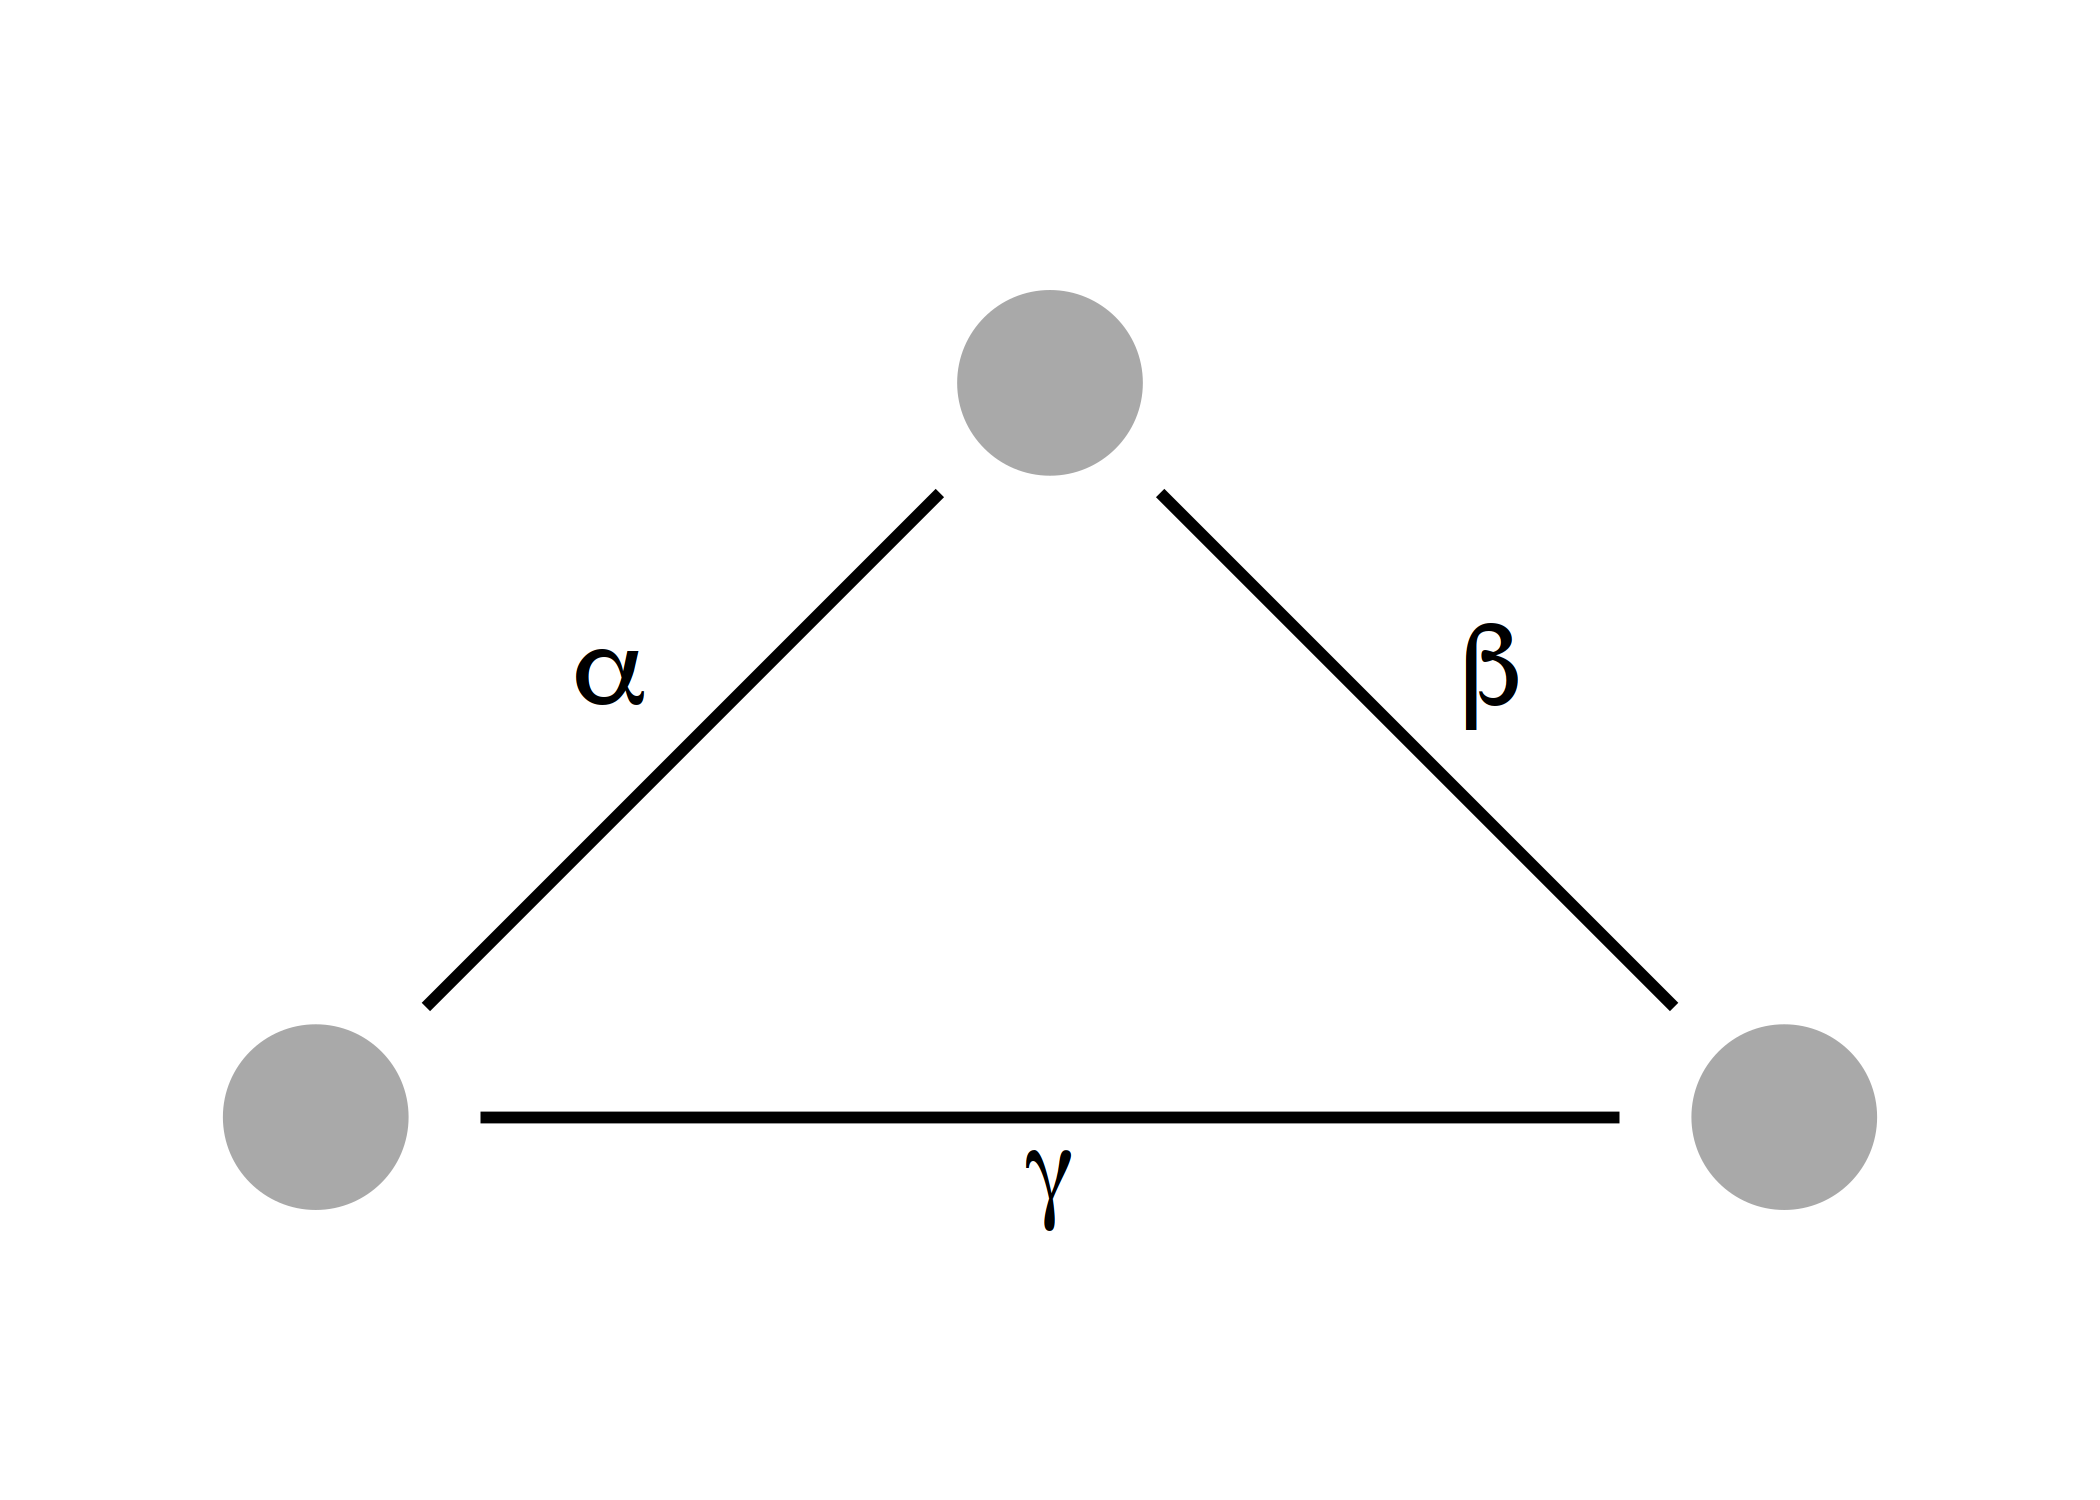
\includegraphics[width=0.8\textwidth]{figures/model-1} 

}

\caption{A mathematical model sets variables (dots) into relation (lines) using parameters.}\label{fig:model}
\end{figure}

The aspects of the world are represented within the model as \emph{variables}.
The blood pressure of a patient is represented with a numerical value.
Images, for example, are represented as tensors of pixels.
Variables can also represent a latent, hidden or abstract aspect.
Like happiness or introversion.
There are different names for variables:
Random variables, covariates, predictors, latent variables, features, target, outcome, \ldots{}
These names sometimes reveal the role of a variable in the model.
For example, the ``target'' is the variable that we want to predict.
In different mindsets, variables have different names and roles:
In machine learning, for example, the terms feature and target are used.
In statistics, people might say dependent and independent variable or covariates and outcome instead.

Within the model, the components are mathematically or computationally set in \emph{relation} to each other.
These relations are usually expressed as parameterized functions.
For example:

\begin{itemize}
\tightlist
\item
  Causal models represent relations between variables in a directed acyclic graph that can be translated into conditional (in-)dependencies.
\item
  The joint distribution of variables describes the occurrence of certain variable values in a probabilist sense.
\item
  A predictive model represents the output variable as a parameterized function of the input variables.
\item
  In the case of a linear regression model, the output variable is a weighted sum of the input variables.
\end{itemize}

The expressive power of such relationships really depends on the class of the model.
A relation can be a simple linear equation like \(Y = 5 \cdot X\) involving two or more variables.
For example we might model the probability of a stroke as a function of blood pressure and age.
A relation can also be a long chain of mathematical operations involving thousands of variables.
Deep neural networks are an example of such a complicated relation.

We don't know the relations between variables in advance, so we use data to learn them.
For some models, learning these relationships is a matter of finding the right \emph{parameters}.
This is true for neural networks and generalized additive models, for example.
For other models, the model structure is ``grown'', as in decision trees or support vector machines.
Growing the structure means not only learning parameters, but also learning the structure of the mathematical function.

You can think of a model as having an uninstantiated state and an instantiated state.
An uninstantiated model is not yet fitted to the data.
Uninstantiated models form families of models.
For example the neural network ResNet architecture, or the family of Poisson regression models.
An instantiated model is trained / learned / fitted using data: It's parameterized and/or the structure has been learned.

I can buy carrots with money.
How many grams of carrots can I get for 1 euro?
Let's call this unknown parameter in our equation \(\beta\):
\(1 \text{ EUR} = \beta \text{ Carrots}\).
I could figure out the \(\beta\) by going to the supermarket and checking the price.
Maybe \(\beta = 500\), so I get half a kilogram of carrots for 1 euro.
But that's only for one supermarket!
Maybe I have to add more variables and relations to the model.
Maybe I need to consider the supermarket chain, special deals, organic / non-organic, \ldots{}
All these choices add variables, relations and parameters to the model.

What we can do with the model depends on the modeling mindset.
In supervised machine learning, we take advantage of the modeled relations to make predictions.
In causal inference, we use our model to estimate causal effects.
In likelihoodism, we can compare the likelihoods between models.

\hypertarget{mindsets}{%
\chapter{Mindsets}\label{mindsets}}

A model is only a bunch of variables, relations, and parameters.
A model alone can't tell us how to interpret the world.
The use and interpretation of the model depends on the mindset from which the model arose.
In order to derive knowledge about the world from the model, we need to make further assumptions.
Consider a linear regression model that predicts regional rice yield as a function of rainfall, temperature, and fertilizer use.
It's a model, not a mindset.
How may we interpret the model?
Can we interpret the effect of fertilizer as causal to rice yield? Or is it just a correlation?
Would we trust the model to make accurate predictions for the future as well?
Can we say anything about the statistical significance of the effect of the fertilizer?
Or have we just updated prior information about the effect of fertilizer with new data?

Welcome to \textbf{Modeling Mindsets}.

A modeling mindset is a specification of how to model the world using data.
Modeling means investigating a real world phenomenon indirectly using a model.\textsuperscript{\protect\hyperlink{ref-weisberg2007modeler}{2}}
Modeling mindsets are like different lenses.
All lenses show us the world, but with a different focus.
Some lenses magnify things that are close, some that are far away.
Some glasses are tinted so you can see in bright environments.
When you look through a lens, you see the world in a certain way.
With different modeling mindsets, you can look at the modeling task, but the model will focus on different things.
Bayesianism, frequentism, supervised machine learning, generative models, \ldots{} these are all different mindsets when it comes to building models from data.
Mindsets differ in how they interpret probabilities -- or whether probabilities are part of the language at all.
While mindsets cover many different modeling tasks, they have some tasks where they really shine.
Each mindset invites you to ask different questions, and so shapes the way you view the world through your model.
In supervised machine learning, for example, everything becomes a prediction or classification problem, while in Bayesian inference, the goal is to update our beliefs about the world using probability theory.

Within a mindset there are two worlds: the model world and the real world (Figure \ref{fig:mindsets}.
Or, as McElreath called them in his book ``Statistical Rethinking'': the ``small'' and the ``large'' world.\textsuperscript{\protect\hyperlink{ref-mcelreath2020statistical}{3}}
All modeling results are first and foremost statements about the model world, and to be interpreted within the simplified model world..
How and if model results may be transferred from the model world to the real world, depends on the mindset.

\begin{figure}

{\centering 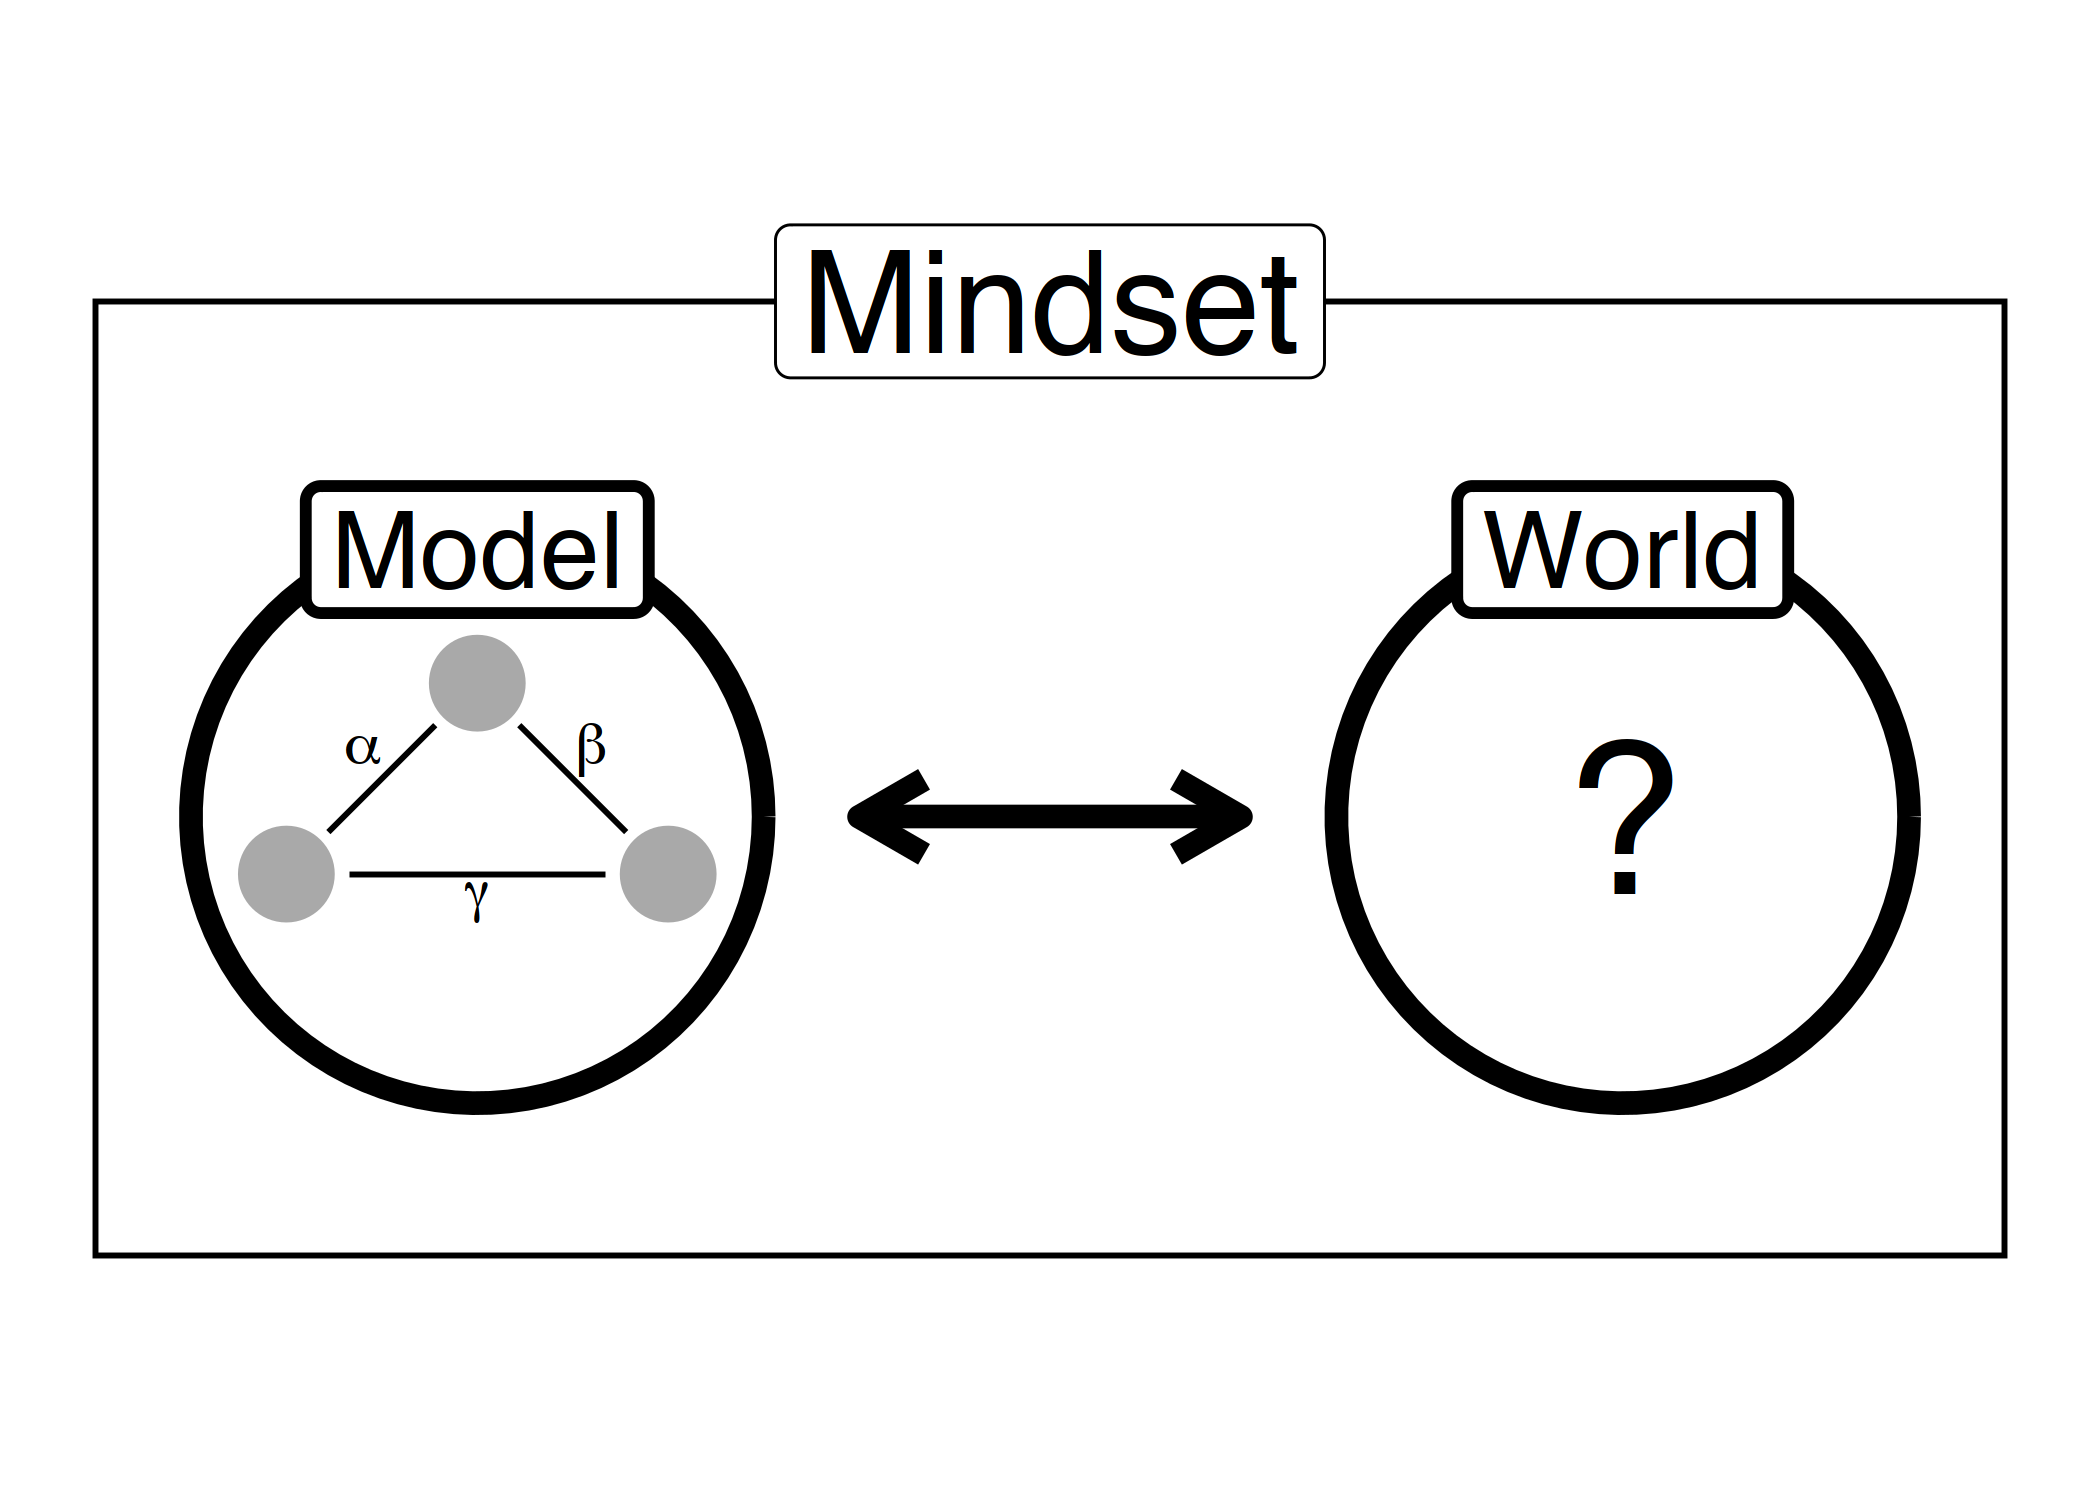
\includegraphics[width=0.8\textwidth]{figures/mindsets-1} 

}

\caption{Only when a model is embedded in a mindset can we put it into context with the world.}\label{fig:mindsets}
\end{figure}

\textbf{Modeling mindsets} are normative:
A modeling mindset distinguishes between good and bad models.
Even though model evaluations are partly based on objective criteria, the choice of a criterion is subjective.
Each mindset has their own set of accepted models and evaluation procedures.

For a frequentist statistician, a good model of the world is probabilistic and has a high goodness-of-fit to the data.
The residual errors of the model also pass diagnostic checks.
The frequentist rejects the use of prior probabilities as they appear to be subjective.
The frequentist would also not switch to a random forest just because it has a lower mean squared error on test data.
And why would the statistician switch?
From their point of view, the random forest is a poor model of the world.
We learn nothing about the probability distribution of our variables.
We can't do frequentist hypothesis testing of the effects of variables.
The performance of the frequentist's model on unseen test data is not as important to the frequentist.

A modeling mindset limits the questions that can be asked.
Consequently, some questions or tasks are out of scope of the mindset.
Often the questions are out of scope because they just don't make sense in a particular modeling mindset.
Supervised machine learners formulate tasks as prediction or classification problems.
Questions about probability distributions are out of reach since the mindset is: choose the model that has the lowest generalization error given new data.
So the best model could be any function, such as the average prediction of a random forest, a neural network, and a linear regression model.
If the best model can be any function, questions that a statistician would normally ask (hypothesis testing, parameter estimation, \ldots) become irrelevant to the machine learner.
In machine learning, the best models are usually not classical statistical models.
If the machine learner started asking questions a statistician would ask, they would have to choose a suboptimal model, which is a violation of the mindset.

\textbf{Modeling mindsets are cultural}.
Modeling mindsets are not just theories; they shape and are shaped by communities of people who model the world based on the mindset.
In many scientific communities, the frequentist mindset is very common.
I once consulted a medical student for his doctoral thesis.
I helped him visualize some data.
A few days later he came back, ``I need p-values with this visualization.''
His advisor told him that any data visualization needed p-values.
His advisor's advice was a bit extreme, and not advice that a real statistician would have given.
However, it serves as a good example of how a community perpetuates a certain mindset.
Likewise, if you were trying to publish a machine learning model in a journal that publishes mostly Bayesian analysis, I would wish you good luck.
And I'd bet 100 bucks that the paper would be rejected.

The people within a shared mindset also accept the assumptions of that mindset.
And these assumptions are usually not challenged, but mutually agreed upon
At least implicitly.
If you work in a team that has been using Bayesian statistics for some time, you won't be questioning each model anew about whether using priors is good or whether the Bayesian interpretation of probability is legit.
In machine learning competitions, the model with the lowest prediction error on new data wins.
You will have a hard time arguing that your model should have won because it's the only causal model.
If you believe that causality is important, you would simply not participate.
You can only thrive in machine learning competitions if you have accepted the supervised machine learning mindset.

The modeling mindsets as I present them in this book are archetypes: pure forms of these mindsets.
In reality, the boundaries between mindsets are much more fluid.
These archetypes of mindsets intermingle within individuals, communities and approaches:
A data scientist who primarily builds machine learning models might also use some simple regression models with hypothesis tests -- without cross-validating the models' generalization error.
A research community could accept analyses that use both frequentist and Bayesian statistics.
A machine learning competition could include a human jury who would award additional points if the model is interpretable and includes causal reasoning.

Have you ever met anyone who is really into supervised machine learning?
The first question they ask is ``Where is the labeled data?''.
The supervised machine learner turns every problem into a prediction or classification problem.
Or perhaps you've worked with a statistician who always wants to run hypothesis tests and regression models?
Or you had intense discussion about probability with a hardcore Bayesian?
Some people really are walking archetypes. 100\% of one archetype.
But I would say that most people learned one or two mindsets when they start out.
And later they got glimpses of other mindsets here and there.
Most people's mindset is already a mixture of multiple modeling mindsets.
And that's a good thing.
Having an open mind about modeling ultimately makes you a better modeler.

\hypertarget{statistical-modeling}{%
\chapter{Statistical Modeling}\label{statistical-modeling}}

\begin{itemize}
\tightlist
\item
  Goal: Changing your mind under uncertainty.
\item
  Assumes the world is best described by probability distributions.
\item
  Requires additional assumptions for drawing conclusions. See \protect\hyperlink{frequentist-inference}{Frequentism Inference}, \protect\hyperlink{bayesian-inference}{Bayesian Inference} and \protect\hyperlink{likelihoodism}{Likelihoodism}.
\item
  \protect\hyperlink{machine-learning}{Machine learning} is an alternative mindset.
\end{itemize}

Do you become more productive when you drink a lot of water?
Is there a fixed ``law'', like a mathematical function, that expresses productivity as a function of water intake?
No.
No, because productivity depends on many factors: sleep duration and quality, distractions, noise pollution, \ldots{}
Because of all these factors and other contingencies, we won't get a perfect equation relating water intake to productivity.
Uncertainty remains.
Even the water intake varies from day to day and from person to person.

Statistics is all about changing your mind under uncertainty.
One way to deal with the uncertainty of the world is to abstract aspects of the world as random variables and ascribe a probability distribution to them.
Daily water intake could be a random variable.
For productivity we would need some clever idea on how to best measure this abstract concept.
A not so clever example: Daily time spent in front of the computer.
To further relate these variables to each other, we can make assumptions on how the data were generated and connect the random variables in a statistical model.

Welcome to the \textbf{statistical modeling} mindset.

A statistical model consists of a set of probability distributions that are fitted to data.
A probability distribution describes the frequency with which we expect to see certain values of random variables.
The second ingredient to a statistical model is the data, from which we estimate those probability distributions.
But let's start with the most elementary unit: the random variable.

\hypertarget{random-variables}{%
\section{Random Variables}\label{random-variables}}

A random variable is a mathematical object that carries uncertainty.
Daily water intake can be a random variable.
Data are seen as \textbf{observations} or realizations of random variables.
If someone drank 2.5 liters of water, that is a realization of the random variable ``daily water intake''.

Other random variables:

\begin{itemize}
\tightlist
\item
  Outcome of a dice roll.
\item
  Monthly sales of an ice cream truck.
\item
  Whether or not a customer has canceled their contract last month.
\item
  Daily amount of rain in Europe.
\item
  Pain level of patients arriving at the emergency room.
\end{itemize}

People with a statistical modeling mindset \textbf{think} in random variables.
Any problem related to data is translated into a set of random variables and solved based on that representation.
A random variable is a construct that we can't observe directly.
But we can observe the realizations of a random variable, as shown in Figure \ref{fig:variable}.
But the raw data are not that useful to humans.
Because humans aren't databases, we need a model that simplifies the noisy data for us.
Statisticians came up with probability distributions: a mathematical construct that describes potential outcomes of the random variable.

\begin{figure}

{\centering 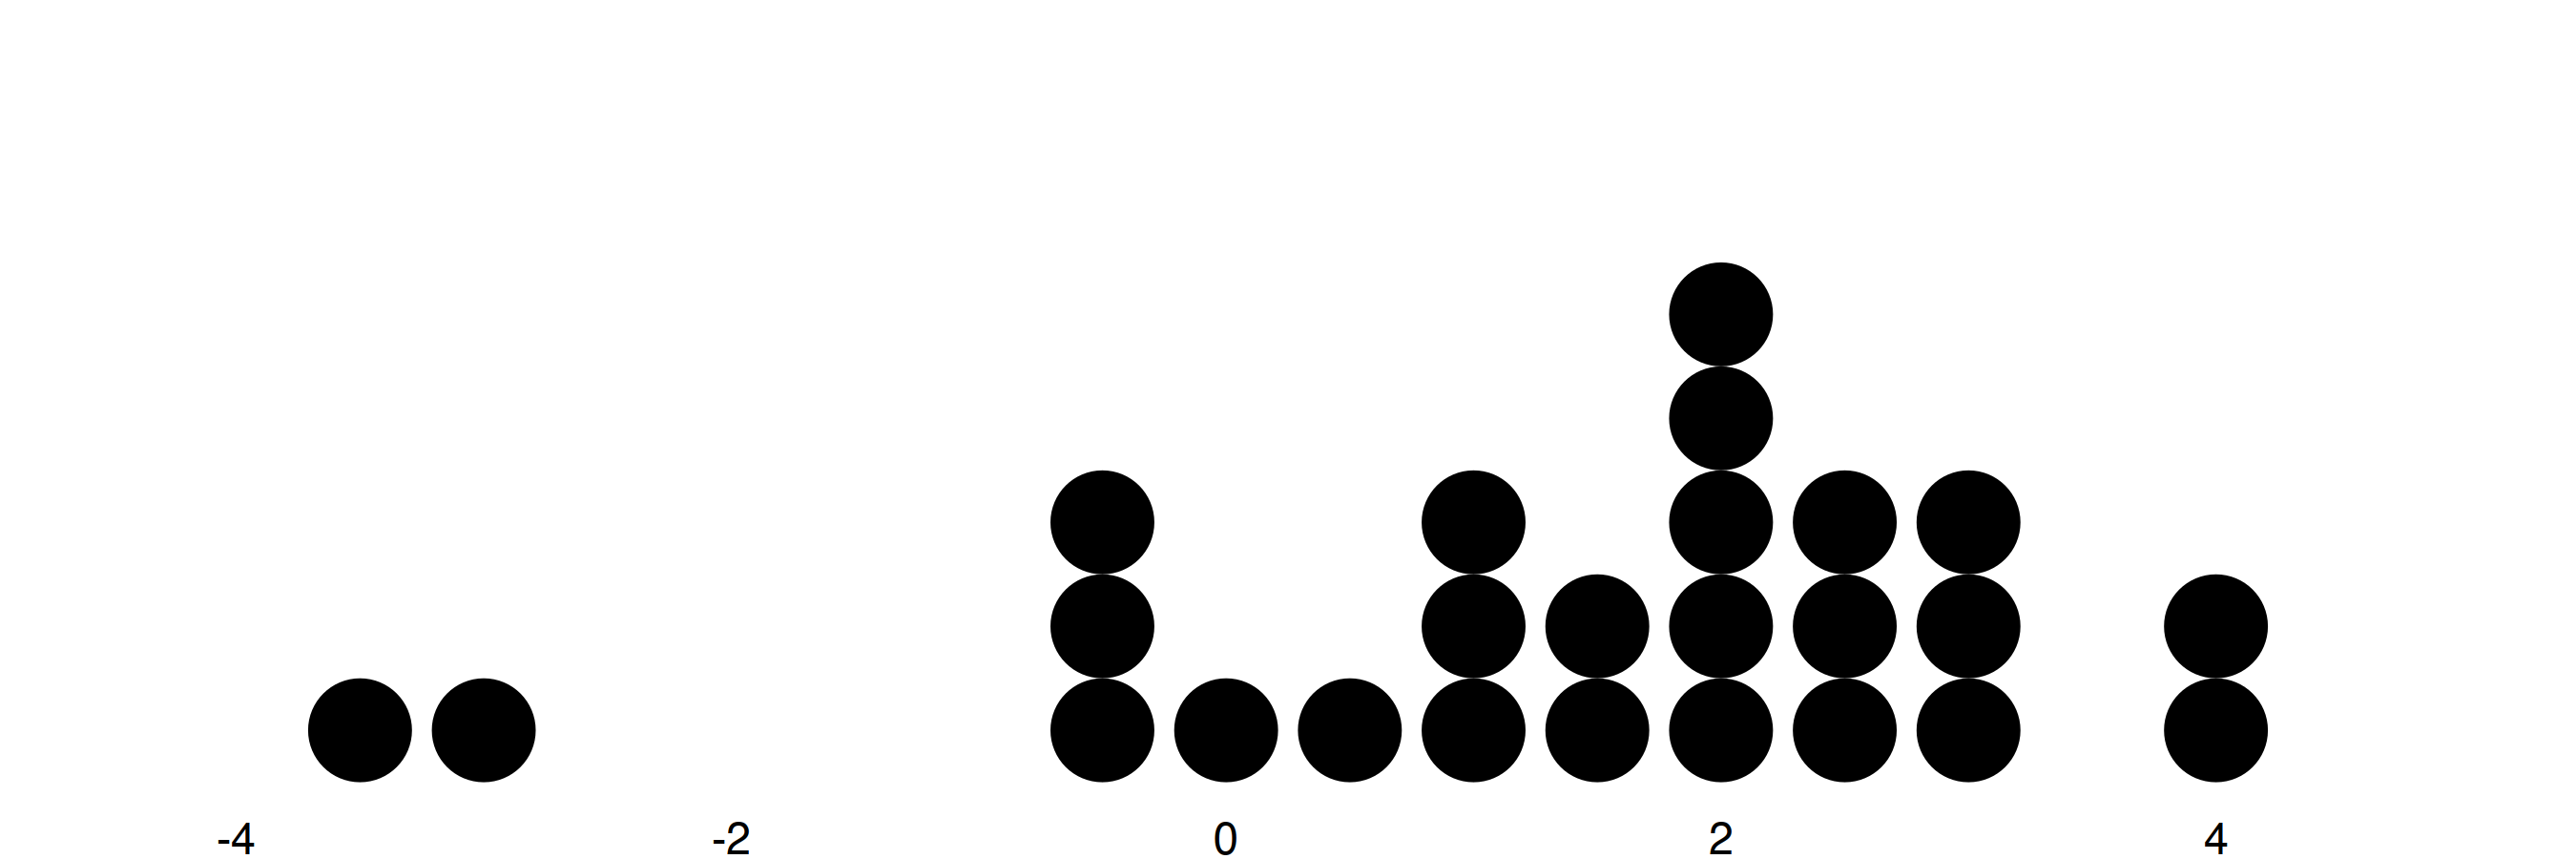
\includegraphics[width=0.8\textwidth]{figures/variable-1} 

}

\caption{Each dot represents a data point, a realizations of a random variable. The x-axis shows the value of the variable. Dots are stacked up for frequently occurring values. }\label{fig:variable}
\end{figure}

\hypertarget{probability-distributions}{%
\section{Probability Distributions}\label{probability-distributions}}

A probability distribution is a function which gives each possible outcome of a random variable a probability.
Value in, probability out.
Not all functions can be used as probability functions.
A probability function must be larger or equal to zero for the entire range of the random variable.
For discrete variables such as the number of fish caught, the probability distribution must sum up to 1 over all possible outcomes.
And for continuous outcomes such as water intake, the probability distribution, also called density function, must integrate to 1 over the possible range of values.

For the outcome \(x\) of a fair dice, we can write the following probability function:

\[
P(x) = 
\begin{cases}
 1/6 & x \in \{1, \ldots, 6\} \\
 0 & x \notin \{1, \ldots, 6\} \\
\end{cases}
\]

The Normal distribution is for continuous variables and defined from minus to plus infinity:

\[f(x) = \frac{1}{\sigma \sqrt{2\pi}} e^{-\frac{1}{2}\left(\frac{x-\mu}{\sigma}\right)^2}\]

In this equation, \(\pi\) and \(e\) are the famous constants \(pi \approx 3.14\) and \(e \approx 2.7\).
The distribution has two parameters: mean \(\mu\) and standard deviation \(\sigma\).
These parameters are sometimes called location (\(\mu\)) and scale (\(\sigma\)) parameters, since they determine where on the x-axis the center of the Normal distribution is and how flat or sharp the distribution is.
The larger the standard deviation \(\sigma\), the flatter the distribution.

Let's try it out and set \(\mu = 0\) and \(\sigma = 1\), as visualized in Figure \ref{fig:distributions}, leftmost curve.
Now we can use this probability distribution function for telling us how probable certain values of our random variable are.
We get \(f(1) \approx 0.24\) and for \(f(2) \approx 0.05\), making \(x=1\) much more likely then \(x=2\).
We may not interpret \(f(x)\) as probability directly.
But we can integrate \(f\) over a region of the random variable to get a probability.
The probability for \(x \in [0.9, 1.1]\) is 4.8\%.

There is huge arsenal of probability distributions: The Normal distribution, the Binomial distribution, the Poisson distribution, \ldots{}
And there is an infinite number of probability distributions that you could invent yourself.

\begin{figure}

{\centering 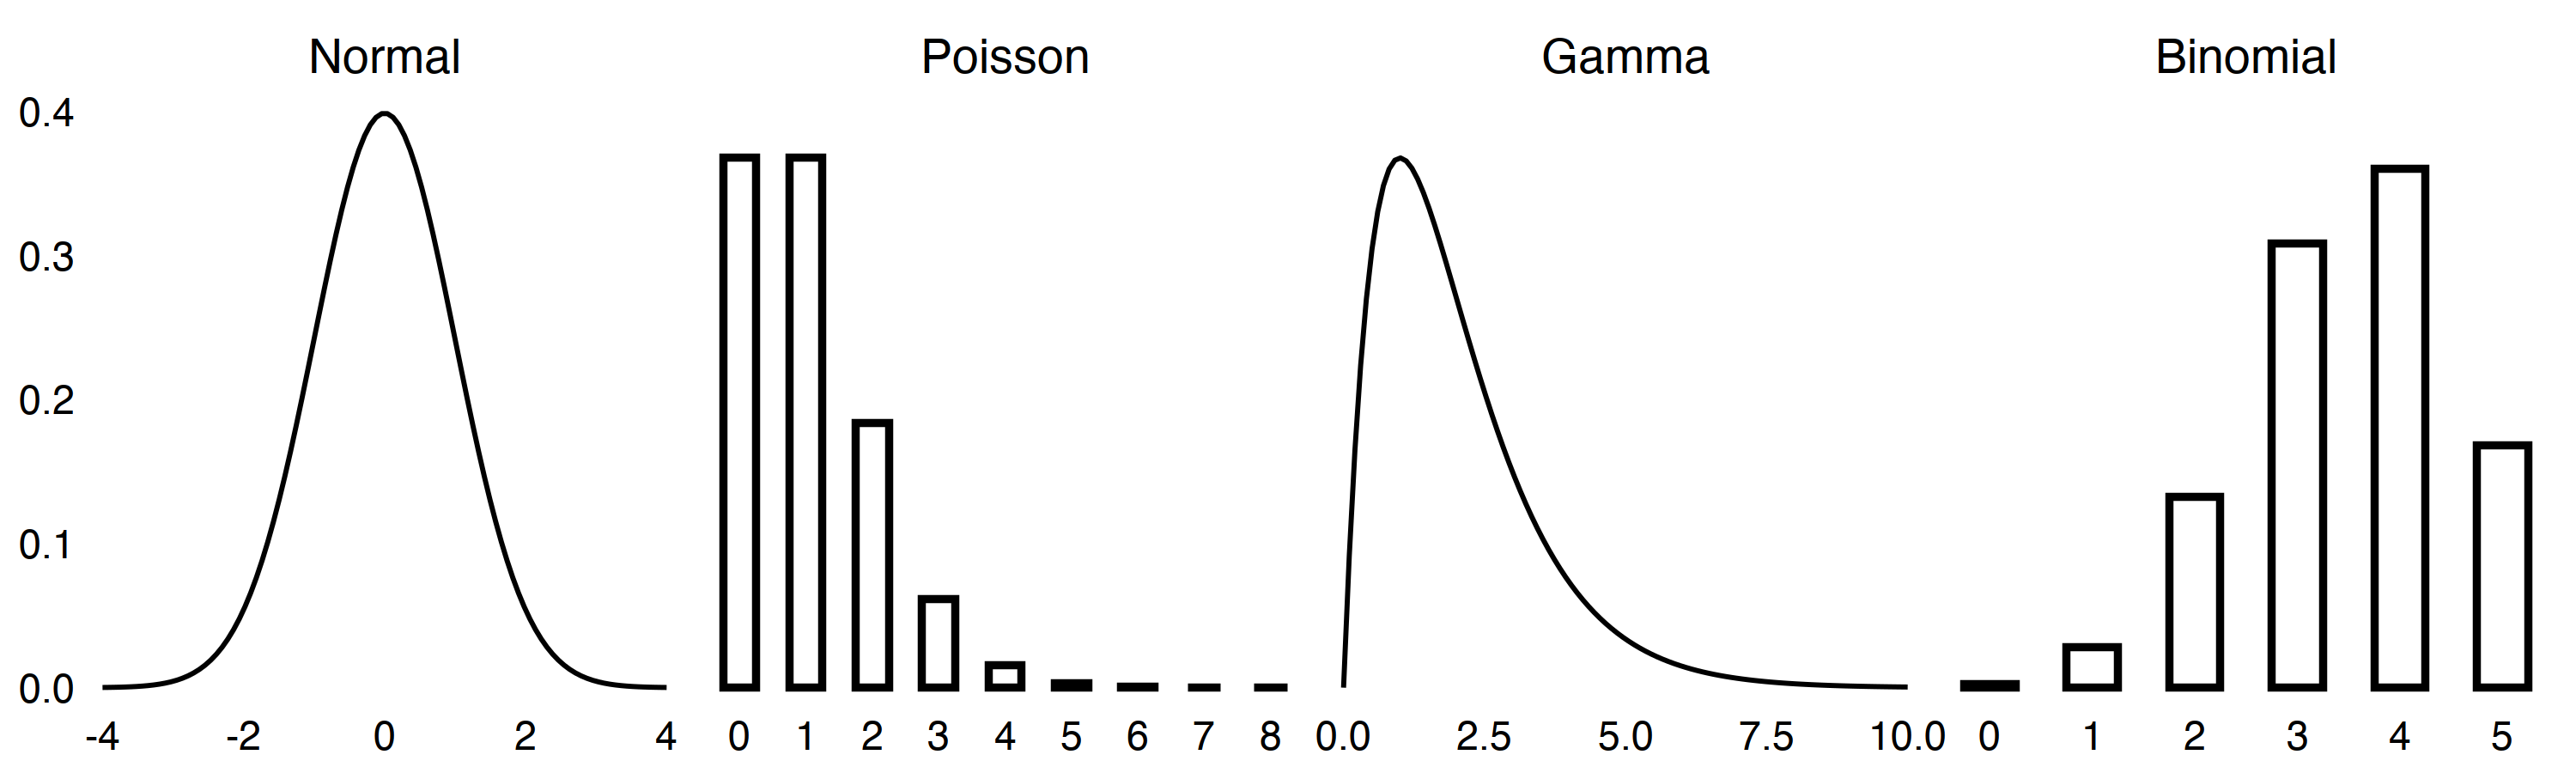
\includegraphics[width=0.8\textwidth]{figures/distributions-1} 

}

\caption{Distributions}\label{fig:distributions}
\end{figure}

\hypertarget{assuming-a-distribution}{%
\section{Assuming a Distribution}\label{assuming-a-distribution}}

An important step in the statistical modeling mindset is to connect the random variables that we are interested in to distributions.
A common approach is to choose a distribution that matches the ``nature'' of your data:

\begin{itemize}
\tightlist
\item
  A numerical outcome such as IQ? That's Normal distribution.
\item
  A count outcome such as number of fish caught in an hour? The Poisson distribution is a solid choice.
\item
  A binary repeated outcome, like the number of successful free throws in basketball? It follows a Binomial distribution.
\end{itemize}

These were examples 1-dimensional distributions that only consider a single variable.
The world is more complex than that:
Random variables can be correlated.
The distribution of one variable can depend on the value that another random variable takes.
Fortunately, it's possible to define so-called multivariate distributions.
A multivariate distribution is a function that takes as input two ore more values and returns a density (still a single number).
We might assume that the joint distribution of water intake and productivity (measured in minutes) follows a 2-dimensional Normal distribution.

Another option is conditional distributions.
For example, we could assume that productivity, conditional on water intake, follows a Normal distribution.

With all these probability distributions, we are still in the realm of abstraction and assumptions.
On one side we have the data: messy and untamed.
On the other side, we have the probability distributions: clean and idealized.
Via random variables we have at least a theory how the two are connected:
The data are the realizations of variables, and distributions summarize the stochastic behaviour of variables.
But we still need to mathematically connect observed data and theoretical distributions.
How can we connect them?

The answer is \textbf{statistical models}.

\hypertarget{statistical-model}{%
\section{Statistical Model}\label{statistical-model}}

A statistical model connects theoretical distributions with observed data.
Statistical models are mathematical models that make assumptions about how the data are generated.
With these assumptions in the background, statistical models are then estimated using data.
More formally, a statistical model is the combination of the sample space from which the data comes from, and a set of probability distributions on this sample space.

The distributions are ``fitted'' to the data by changing the parameters.
Imagine the distribution as a cat.
And your data is a box.
Your cat fits it's shape and position to match the box.

How does the cat know which form to take on?
Ah pardon, our question now is:
How do we find parameter values so that the distribution fits the data well?
The density function of the Normal distribution, for example, has mean and variance as parameters.
Given the parameters, the density or probability function can tell us how likely certain values of our random variables are.

We can also use the probability or density function to find our parameters -- by reversing the point of view and calling it the likelihood function.
The value of the random variable is the input of the probability function, and the parameters are seen as given.
The likelihood function \(L(\theta, X)\) is equal to the probability function.
Except that the parameters are now the input, and the values of the random variable are seen as given.
They are given, in the sense that we have data that are realizations of the random variable.

We can take an observed value for \(X\) from our data and plug it into the likelihood function.
Now we have a likelihood function that can tell us, for this one data point, which parameters would give the highest probability for observed this particular value.
But our data consist of multiple realizations of random variables.
To get the likelihood for the entire dataset, we multiply the likelihoods of the individual data points.
This data likelihood can tell us, for a given parameter value, how likely our data is.
For example we could try \(\mu = 1\) and \(\sigma = 2\) and the likelihood function returns a value.
The larger the value, the better the distribution (with these parameters) fits the data.
That's very useful, because it helps us in finding the best parameters.

Finding the best parameters is a classical optimization problem:
Maximize the data likelihood \(L\) with respect to the parameters.
We want to maximize the likelihood for all of our data: \(L(\theta, \mathbf{x}_1, \ldots, \mathbf{x}_n) = \prod_{i=1}^n L_i(\theta, \mathbf{x}_i)\).
Note that \(\mathbf{x}_i\) can be a vector with values for multiple variables.
And we maximize the data likelihood:

\[\arg \max_{\theta} L(\theta | \mathbf{x}_1, \ldots, \mathbf{x}_n)\]

\hypertarget{maximum-likelihood-estimation}{%
\subsection*{Maximum Likelihood Estimation}\label{maximum-likelihood-estimation}}


Maximum likelihood estimation is a classic optimization problem.
For simpler cases this can even be solved analytically.
For the Normal distribution, we know that the optimal \(mu\) is the mean of the data: \(\frac{1}{n} \sum_{i=1}^n x_i\).
When an analytical solution is not possible, other optimization methods like gradient descent, the Newton-Raphson method and Fisher's scoring can be used.

Maximum likelihood estimation is a key element to understanding the statistical modeling mindset.
Maximizing the likelihood means bringing together the theoretical probability distributions and the observed data.

\begin{figure}

{\centering 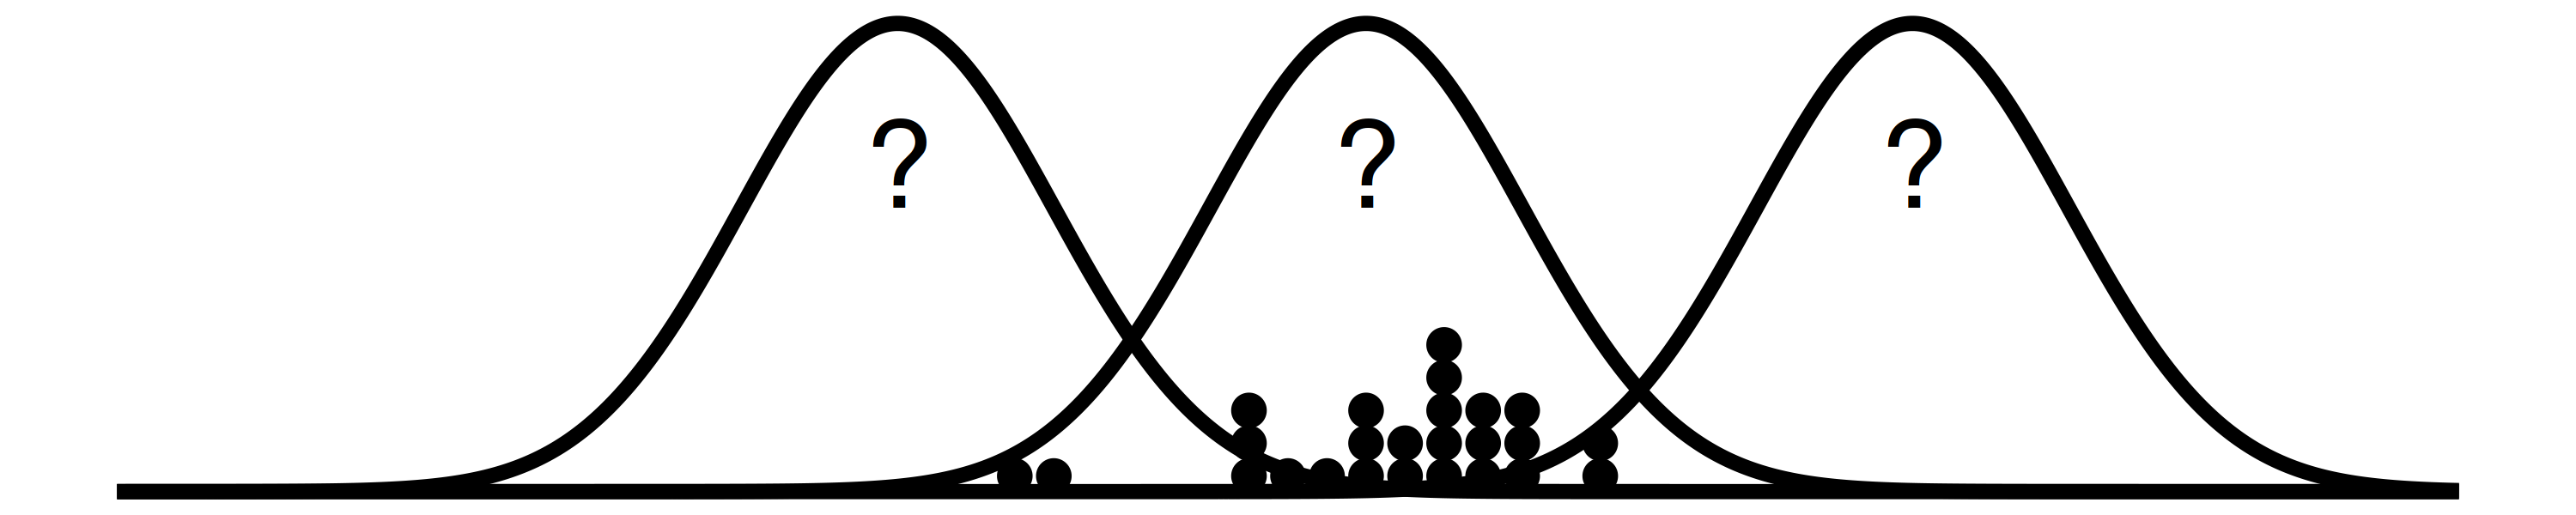
\includegraphics[width=0.8\textwidth]{figures/fit-1} 

}

\caption{Fitting distributions to data}\label{fig:fit}
\end{figure}

\hypertarget{statistical-hypothesis}{%
\subsection*{Statistical Hypothesis}\label{statistical-hypothesis}}


A statistical hypothesis is a specification of a probability distribution for (observable) random variables.
A statistical model can also embody a statistical hypthesis, because it specifies a probability distribution.
For example, saying that the height of people follows a Gaussian distribution is a statistical hypothesis.
The effect of a drug on disease progression could be modeled with a logistic regression model.
After the model was fitted, the resulting statistical model also represents a statistical hypothesis.
An alternative statistical hypothesis would be that the effect of the drug is zero, which also encodes a statistical model.

As you can see there is a tight relationship between statistical models and statistical hypotheses.
All statistical models can be your statistical hypotheses.
But a statistical hypothesis is not necessarily fitted with data, or at least parts are manipulated.
A statistical hypothesis can come purely from data plus the modeling assumptions.
Or it can be purely come from assumptions.
Or something inbetween, that some parameters from a statistical model are fitted, the other are assumed to take on a certain value.

What we do with those hyptotheses depends on the mindset.
Frequentist inference engages in null hypothesis significance testing: Define an alternative hypothesis to your statistical model (which is a hypothesis); then computed the probability to observe your model under the alternative hypothesis (= p-value).
Likelihoodism compares the likelihoods of two statistical hypothesis.
In Bayesian inference we can compare the Bayes factor to compare two hypothesis.

\hypertarget{interpreting-parameters}{%
\subsection*{Interpreting Parameters}\label{interpreting-parameters}}


The parameters are not only things to be optimized.
Their role goes beyond that of a mere technical controller.
The parameters are central to the statistical modeling mindset.

\textbf{Statisticians interpret the parameters as summary of the data.}

Statistical modeling is about understanding our data better.
The nice consequence of modeling the data with probability distributions is that we summarize our data with just a few numbers, the parameters.
In the case of the Normal distribution, we can describe the distribution of a single variable with only two numbers, the mean and the standard deviation.
Also for other types of statistical models, parameters are central to interpretation.

\hypertarget{joint-or-conditional-distribution}{%
\section{Joint or Conditional Distribution}\label{joint-or-conditional-distribution}}

All statistical models target an aspect of a probability distribution.
For most of the chapter, we talked about simpler cases, like the distribution of a single variable: \(P(X)\).
But we could have the case of multiple random variables \(X_1, \ldots, X_p\).
To describe the full distribution of more than one variable, we have to work with the joint distribution.

A Gaussian mixture model, for example, requires learning the entire distribution of multiple variables.
Gaussian mixture models can be used for identifying clusters in the data, which are assumed to stem from a mixture of Normal distributions.
Gaussian mixture models are also an example of using a different optimization algorithm than the maximum likelihood algorithm: the expectation-maximization algorithm, which iteratively jumps between optimizing the model parameters and predicting the ``mixture'' of cluster centers for each data point.

The joint distribution is not always of interest and can be difficult to estimate.
It's often much simpler to work with \emph{conditional distributions}.
The conditional distribution tells us how likely the outcome of one or more random variables is given that we already know the values of some other random variables.
For example:

\begin{itemize}
\tightlist
\item
  Which risk factors influence the probability of getting lung cancer?
\item
  How do climatic conditions like temperature and humidity affect the occurrence of bonobos?
\item
  On what days is a hospital likely to be understaffed?
\end{itemize}

The conditional distribution is the natural form for prediction tasks.
And it's usually simpler to estimate than the joint distribution.
Models of the conditional distribution are central to statistical modeling.
They are also known as regression models.

\hypertarget{regression-models}{%
\section{Regression Models}\label{regression-models}}

Regression models are statistical models of the conditional and not the joint distribution.
Let's say we have two variables: \(Y\) and \(X\).
With the joint distribution \(P(Y,X)\) we could answer ``How likely is it that \(X=x\) and \(Y=y\) occur together?
But with the conditional distribution we can ask:''Given \(X=x\), how likely are certain values for \(Y\)``?

For example, we want to know not only how often a disease is successfully treated.
We might want to know if a certain drug played a part in the disease outcome.
Other factors such as the patient's age, disease progression, etc. may play a role.

Our target is the distribution of outcome variable \(Y\) conditional on variables \(X_1, \ldots, X_p\).
Within the regression model, the distribution of \(Y\) is linked to the variables \(X_1, \ldots, X_p\).
Often this means that we express the parameters \(\theta\) of \(Y\)'s distribution (such as the mean \(\mu\) in a Normal distribution) as a function of the other variables.
How exactly this link looks like depends on the distribution that the modeler assumed for \(Y\) and the link they chose to connect \(\theta\) and \(X\).
The simplest case is a linear regression model.
We assume that \(Y\) follows a Normal distribution and link the mean of \(Y\)'s distribution to a weighted sum of the other variables:

\[Y \sim N(\mu, \sigma)\]

\[\mu = \beta_0 + \beta_1 X_1 + \ldots + \beta_p X_p\]

The linear regression model expresses the mean of the target \(Y\) as the weighted sum of the other variables.
\(Y\) given \(\mathbf{X}\) follows a Normal distribution.
We only link the mean \(\mu\) to the variables.
A typical assumption is that the standard deviation \(\sigma\) is independent of the value of the other variables.

What can we do now with a regression model?
We can make predictions.
We just have to fill in values for \(X\) and get the expected value of the probability distribution of \(Y\).
While the conditional mean of \(Y\) is often the goal of the regression model, the statistician can also target other parts of the conditional distribution.
For example the median or other quantiles.
These types of regression models are quantile regression models.
For survival models the target is often the hazard rate, which is a function of the probability of an event happening in a time interval.
See for example the Cox proportional odds model.

\textbf{Interpretation of parameters} is usually even more important than prediction.
The parameters contain information about the relationship between the target and the other variables.
For regression models, we usually speak of the coefficients.
In the linear regression model, a positive coefficient \(\beta_j\) means that increasing the value of variable \(X_j\) increases the expected value of \(Y\).

A large part of statistical modeling consists of regression models in different flavors.

\begin{itemize}
\tightlist
\item
  Generalized linear models (GLMs)
\item
  Generalized additive models (GAMs)
\item
  Quantile regression
\item
  Mixed effect models
\item
  \ldots{}
\end{itemize}

Most of these models were ``invented'' to address a shortcoming of another regression model.
GLMs can model targets that don't follow a Normal distribution but some other distribution.
GAMs can model non-linear relationships.

Regression models also have a place in \protect\hyperlink{supervised-ml}{supervised machine learning}.
But in supervised machine learning, the goal is to achieve good predictive performance on unseen data.
And if a random forest performs better than a GAM, then the GAM gets thrown out, even if it has nicer statistical properties.

\hypertarget{model-evaluation}{%
\section{Model Evaluation}\label{model-evaluation}}

Good statisticians evaluate their models.
Understanding how this evaluation works will help you better understand the statistical modeling mindset.
It's particularly interesting to see how much the evaluation in the statistical modeling mindset differs from that of \protect\hyperlink{supervised-ml}{supervised machine learning}.
The evaluation of statistical models consists of two parts: \textbf{model diagnostics and goodness-of-fit}.

The role of model diagnostics is to check whether the modeling assumptions were reasonable.
If we have assumed that a random variable follows a Normal distribution, we can check this assumption visually.
For example, with a Q-Q plot.
Another typical assumption is homoscedasticity: The variance of the target is independent of other variables.
Homoscedasticity can be checked visually by plotting the residuals (\(y_i\) minus its predicted value) against each of the other variables.

A model that passes these diagnostics is not automatically a good model.
Statisticians use goodness-of-fit measures to compare models and evaluate modeling choices, such as which variables to have in the model.\\
Typical goodness-of-fit measures are the (adjusted) R-squared, Akaikes Information Criterion (AIC), the Bayes factor, and likelihood ratios.
Goodness-of-fit is literally a measure of how well the model fits the data.
The goodness-of-fit can guide the model building process and decide which model is chosen in the end.

Goodness-of-fit is typically computed with the same data that were used for fitting the statistical models.
This choice may look like a minor detail, but it says a lot about the statistical modeling mindset.
The critical factor here is overfitting: The more flexible a model is, the better it adapts to ALL the randomness in the data instead of learning patterns that generalize.
Many goodness-of-fit metrics therefore account for model complexity, like the AIC or adjusted R-squared.
Compare this to \protect\hyperlink{supervised-ml}{supervised machine learning}: in this mindset, there is a strict requirement to always use ``fresh'' data for evaluation.

\hypertarget{data-generating-process-dgp}{%
\section{Data-Generating Process (DGP)}\label{data-generating-process-dgp}}

A quite central, but fuzzy also topic of the statistical modeling mindset is the data-generating process.
The statistical modeler thinks about the data-generating process all the time.
The data-generating process is a construct, an unknowable ideal of how the data were generated.
The data-generating process produces the unknown distributions that then produce the data.
We observe the data-generating process indirectly through the data.
With data and reflections on the DGP, sometimes together with experts, the statistician tries to decipher the DGP.
Statisticians talk about the DGP all the time, but it remains more of a mental model than a clearly defined concept.
When I was studying statistics, the DGP was mentioned in most lectures.
But I never had a formal lecture on what the DGP is.
It's also difficult to find textbooks, lectures, or blog posts that define what the DGP really is.
It seems to me that the mental model of a DGP is a natural consequence of viewing the world in terms of probability distributions.

The DGP is a powerful idea, even if it's not well defined.
Assuming a DGP encourages you to intellectually dive deep into your data.
Having this image of a DGP in your mind let's you take on the mindset of a detective:
Statisticians are like detectives reconstructing a crime.
You can't observe the crime directly.
But the crime has generated a lot of ``data'' at the scene.
The stats detective then tries to uncover the data-generating process by making assumptions and learning from the observed data.

There is no definition of the data-generating process, so I'll give you a some examples:

\begin{itemize}
\tightlist
\item
  Rolling dice is a data-generating process. A die is symmetric, making each side equally likely. We could factor in the angle of the throw, surface roughness and so on. But the chaotic behaviour of the dice bouncing and spinning across the table makes us disregard all these factors.
\item
  We study the income of computer scientists via a survey. Instead of mindlessly reporting the income distribution, we think about the entire data-generating process: For example, some income values are missing. Are they missing at random? Are higher-income individuals more likely to leave the income answer empty? Are some businesses overrepresented in the survey? Is the sample truly random?
\item
  A research team has collected chest x-ray images of patients with and without COVID-19 for building a COVID-19 prediction model. A closer look at the data-generating process shows: the images not only differ in COVID-19 status, but they come from different data-generating processes. COVID-19 images are often taken with patients lying down because of exhaustion. One of the non-COVID-19 datasets are even children x-ray images.\footnote{Wynants, Laure, Ben Van Calster, Gary S. Collins, Richard D. Riley, Georg Heinze, Ewoud Schuit, Marc MJ Bonten et al.~``Prediction models for diagnosis and prognosis of covid-19: systematic review and critical appraisal.'' bmj 369 (2020).} Considering the DGP casts doubt on whether such data can be used to build a COVID-19 classifier or whether, in reality, it classifies data into child/adult, standing/lying down, \ldots{} I chose this example because it's a paper from the \protect\hyperlink{supervised-ml}{supervised machine learning mindset}. A good statisticians would check the DGP much more carefully, making it more likely to detect such problems.
\end{itemize}

If these examples of data-generating processes sound like common sense to you, it's because they are.
But it's surprisingly uncommon among non-statistician mindsets.
For example, for \protect\hyperlink{supervised-ml}{supervised machine learning}, considerations of the data-generating process play a subordinate .
For most machine learning competitions the winner is determined solely by the lowest prediction error on new data.
It doesn't matter whether the model meaningfully reflects the data-generating process.

\hypertarget{drawing-conclusions-about-the-world}{%
\section{Drawing Conclusions About the World}\label{drawing-conclusions-about-the-world}}

In most cases, statistical models are built for practical reasons:
To make a decision, to better understand some property of the world, or to make a prediction.
These goals require the interpretation of the model instead of the world.
But using the model as a representation of the world isn't for free.
The statistician must consider the representativeness of the data and choose a mindset that allows the findings of the model to be applied to the world.

Considering the data-generating process also means thinking about the representativeness of the data, and thus the model.
Are the data a good sample and representative of the quantity of the world the statistician is interested in?
Let's say a statistical modeler analyzes data on whether a sepsis screening tool successfully reduced the incidence of sepsis in a hospital.
They conclude that the sepsis screening tool has helped reduce sepsis-related deaths at that hospital.
Are the data representative of all hospitals in the region, the country, or even the world?
Are the data even representative of all patients at the hospital, or are data only available from patients in intensive care unit?
A good statistical modeler define and discuss the ``population'' from which the data are a sample of.
\protect\hyperlink{design-based-inference}{Design-based inference} fully embraces this mindset that the data are sampled from a larger population.

More philosophical is the modeler's attitude toward causality, the nature of probability, and the likelihood principle.

\begin{quote}
``It is unanimously agreed that statistics depends somehow on probability. But, as to what probability is and how it is connected with statistics, there has seldom been such complete disagreement and breakdown of communication since the Tower of Babel.''
\end{quote}

-- Leonard Savage, 1972\footnote{Savage, Leonard J. The foundations of statistics. Courier Corporation, 1972.}

Statistical modeling is the foundation for learning from data.
But we need another mindset on top of that to make the models useful.

\protect\hyperlink{frequentism-frequentism}{Frequentist inference} is the most prominent mindset for inferring properties about the world from statistical models.
Frequentist statistics sees probability as relative frequencies of events in long-run experiments.

\protect\hyperlink{bayesian-inference}{Bayesian inference} is based on an interpretation of probability as a degree belief about the world.
Bayesianism states that the model parameters also have a (prior) distribution.
And the goal of the statistician is to update the prior distribution by learning from data.
The resulting posteriori distributions of the parameters express our belief about the world.

\protect\hyperlink{likelihoodism}{Likelihoodism} is a lesser known modeling mindset. Like Bayesianism, it adheres to the likelihood principle, which states that the likelihood function captures all evidence from the data (which frequentist inference violates).
However, it does not require prior probabilities.

\protect\hyperlink{causal-inference}{Causal inference} adds causality to statistical modeling. It can be superimposed onto any of the other three mindsets.

A different but complimentary approach is \protect\hyperlink{design-based-infernce}{design-based inference}, which focuses on data sampling and experiments instead of models.

\hypertarget{strengths}{%
\section{Strengths}\label{strengths}}

\begin{itemize}
\tightlist
\item
  The statistical modeling mindset is a \emph{language to see the world}. Even when not used for inference, random variables and probability distributions are useful mental models for perceiving the world.
\item
  Statistical modeling has a long tradition and extensive theoretical foundation, from measurement theory as the basis of probability theory to convergence properties of statistical estimators.
\item
  The data-generating process is an underestimated mental model. But it's a powerful mental model that encourages mindful modeling and asking the right questions.
\item
  Conditional probability models can be used not only to learn about the parameters of interest, but also to make predictions
\item
  Probability distributions give us a language to express uncertainty. \protect\hyperlink{bayesian-inference}{Bayesianism} arguably has the most principled focus on formalizing and modeling uncertainty.
\item
  Can naturally handle different types of variables: Categorical, ordinal, numerical, \ldots{}
\end{itemize}

\hypertarget{limitations}{%
\section{Limitations}\label{limitations}}

\begin{itemize}
\tightlist
\item
  Statistical modeling reaches its limits whenever defining probability distributions becomes difficult. Images and text don't easily fit into this mindset, and this where \protect\hyperlink{supervised-ml}{supervised machine learning} and especially \protect\hyperlink{deep-learning}{deep learning} shine.
\item
  Working within the statistical modeling mindset can be quite ``manual'' and tedious. It's not easy to always think about the DGP, and sometimes more automatable mindsets such as supervised machine learning are more convenient.
\item
  Statistical models require a lot of assumptions. Sometimes more, sometimes less. Just to name a few common assumptions: homoscedasticity, independent and identically distributed data (IID), linearity, independence of errors, lack of (perfect) multicollinearity, \ldots{} For most violations, there is a special version of a statistical model that doesn't require the critical assumption. The price is more complex and less interpretable models.
\item
  Statistical modeling, when used for prediction, is often outperformed by \protect\hyperlink{supervised-ml}{supervised machine learning}. To be fair, outperforming here requires an evaluation based on the supervised learning mindset. However, this means that goodness-of-fit and diagnosis are no guarantee that a model will performs well on all metrics.
\end{itemize}

\hypertarget{frequentist-inference}{%
\chapter{Frequentist Inference}\label{frequentist-inference}}

\begin{itemize}
\tightlist
\item
  Popular modeling mindset in science.
\item
  The world consists of probability distributions with fixed parameters that have to be uncovered.
\item
  Interprets probability as long-run relative frequencies from which hypothesis tests, confidence intervals and p-values are derived.
\item
  A statistical mindset, with \protect\hyperlink{bayesian-inference}{Bayesian inference} and \protect\hyperlink{likelihoodism}{likelihoodism} as alternatives.
\end{itemize}

Drinking alcohol is associated with a higher risk of diabetes in middle-aged men.
At least this is what a study claims.\textsuperscript{\protect\hyperlink{ref-kao2001alcohol}{4}}

The study modeled type II diabetes as a function of various risk factors.
The researchers found out that alcohol significantly increases the diabetes risk for middle-aged men by a factor of \(1.81\).

``Significant'' and ``associated with'' are familiar terms when reading about scientific results.
The researchers in the study used a popular modeling mindset to draw conclusions from the data: frequentist inference.
There is no particular reason why I chose this study other than it is not exceptional.
When someone thinks in significance levels, p-values, hypothesis tests, null hypotheses, and confidence intervals, they are probably frequentist.

In many scientific fields, such as medicine and psychology, frequentist inference is the dominant mindset.
All frequentist papers follow similar patterns, make similar assumptions, and contain similar tables and figures.
Knowing how to interpret model coefficients, confidence intervals and p-values is like a key to contemporary scientific progress.
Or at least a good part of it.
Frequentism not only dominates science, but has a firm foothold in industry as well:
Statisticians, data scientists, and whatever the role will be called in the future, use frequentist inference to create value for businesses:
From analyzing A/B tests for a website to calculating portfolio risk to monitoring quality on production lines.

As much as frequentism dominates the world of data, it's also criticized.
Frequentist inference has been the analysis method for scientific ``findings'' that turned out to be a waste of research time.
You may have heard about the replication crisis.\textsuperscript{\protect\hyperlink{ref-ioannidis2005most}{5}}
Many scientific findings in psychology, medicine, social sciences and other fields could not be replicated.
The problem with that is that replication is at the center of the scientific method.
Many causes have contributed to the replication crisis
But frequentist statistics is right in the middle of it.
The frequentist mindset enables practices such as multiple testing and p-hacking.
Mix this with the pressure on academics to ``publish or perish''.
The result is a community that is incentivized to squeeze out ``significant'' results at a high rate.
Frequentism is a decision-focused mindset and can give seemingly simple yes/no answers.
Humans are lazy.
So we tend to forget all the footnotes and remarks that come with the model.

Frequentist inference is a statistical modeling mindset:
It depends on random variables, probability distributions, and statistical models.
But as mentioned in the chapter \protect\hyperlink{statistical-modeling}{Statistical Modeling}, these ingredients are not sufficient to make statements about the world.

Frequentism comes with a specific interpretation of probability:
Probability is seen as the relative frequency of an event in infinitely repeated trials.
That's why it's called frequentism: frequentist inference emphasizes the (relative) frequency of events.
But how do these long-run frequencies help to gain insights from the model?

Let's go back to the \(1.81\) increase in diabetes risk among men who drink a lot of alcohol.
\(1.81\) is larger than \(1\), so there seems to be a difference between men who drink alcohol and the ones who don't.
But how can the researchers be sure that the \(1.81\) is not a random result?
For fair dice, the average eyes in the long-run series of experiments is 3.5.
If I roll a die 10 times and the average is 4, would you say it's an unfair die?
No? Would you say it's unfair if the average is 4.5? 5? Or if a 6 shows up 10 times?

The researchers applied frequentist thinking to decide between randomness and true effects.
The parameter of interest is a coefficient in a logistic regression model.
The logistic regression model links variables such as alcohol to diabetes.
In the diabetes study, a 95\% confidence interval for the alcohol coefficient was reported:
The interval goes from \(1.14\) to \(2.92\).
This interval settles the question of randomness versus signal:
The interval doesn't contain \(1\), and so the researchers concluded that alcohol is a risk factor for diabetes (in men).
This confidence interval describes uncertainty regarding the alcohol coefficient.
If we were to repeat the analysis many times with new samples, the respective 95\% confidence interval would cover the ``true'' parameter 95\% of the time.
Always under the condition that the model assumptions were correct.

\hypertarget{frequentist-probability}{%
\section{Frequentist probability}\label{frequentist-probability}}

The interpretation of the confidence interval reveals the \textbf{core philosophy of frequentism}:

\begin{itemize}
\tightlist
\item
  The world can be described by probability distributions;
\item
  The parameters of the probability distributions are constant and unknown;
\item
  Repeated measurements/experiments reveal the true parameter values in the long-run.
\end{itemize}

In contrast, \protect\hyperlink{bayesian-inference}{Bayesianism} assumes that the parameters of the distributions are themselves random variables.
As the frequentists collect more and more data (\(n \to \infty\)), their parameter estimation gets closer and closer to the true parameter (if the estimator is unbiased).
With each additional data point, the uncertainty of the estimated parameter shrinks and the confidence interval becomes narrower.

The frequentist interpretation of probability requires imagination.
Frequentists start with a population in mind.
The population can be adults between 20 and 29 living in Iceland, daily measurements of water quality of the Nile River, or 1-inch wood screws manufactured in a factory in the U.S. state of Texas.
These populations can be described by finding out their probability distributions.
Going back to the initial example:
What's the probability that a middle-aged man will develop diabetes in the next 12 months?
Frequentists would say: There is an unknown and fixed probability for diabetes.
The more people we observe, the more accurate our estimate of the probability of diabetes becomes.
We estimate the probability of diabetes as the relative frequency of diabetes in the population.
Probabilities are frequencies in the long-run:

\[P(X=1) = \lim_{n \mapsto \infty} \frac{1}{n}\sum_{i=1}^{n} I(x_i = 1)\].

\begin{figure}

{\centering 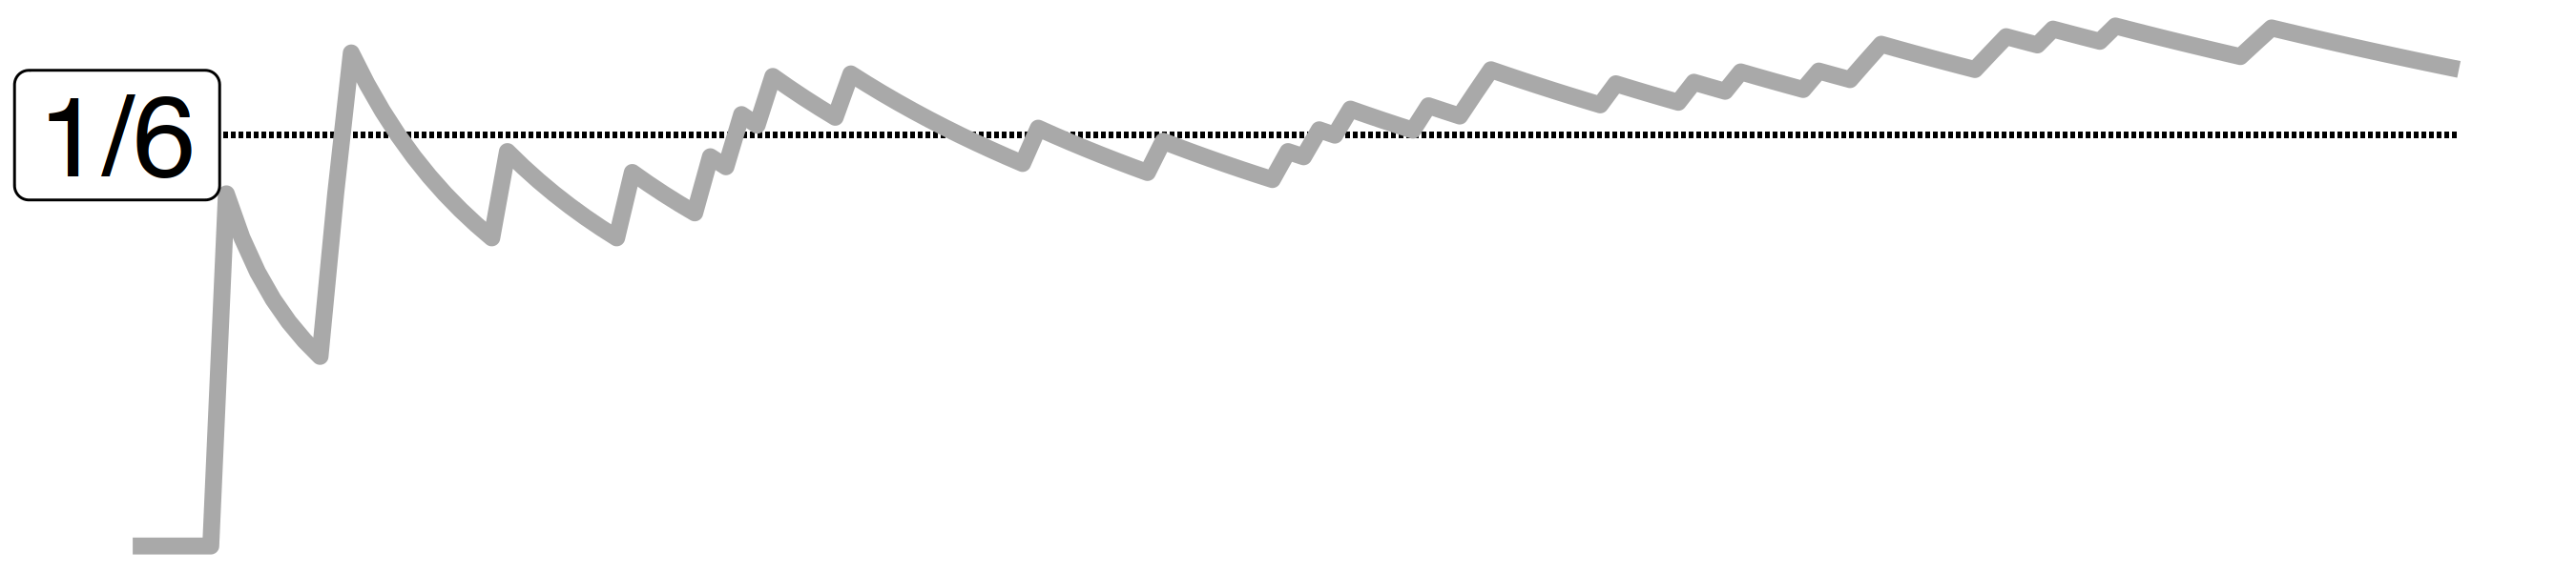
\includegraphics[width=0.8\textwidth]{figures/dice-1} 

}

\caption{The line shows how the relative frequency of 6 eyes changes as the number of dice roles increases from 1 to 100 (left to right).}\label{fig:dice}
\end{figure}

Imagining experiments that will never take place is essential to the frequentist mindset.
By defining probability in terms of long-run frequencies, frequentism requires imagining that the sampling and experiment will be done many times.
These ``imagined'' experiments are central to the interpretation of confidence intervals, p-values, and hypothesis tests.
And \emph{every} interpretation of probability in the frequentist mindset has to be connected to frequencies of events in long-run samples / experiments.

These imagined experiments have a curious implication for frequentism.
Frequentism violates the likelihood principle, which says that all evidence about the data is contained in the likelihood function.
But with frequentism, it's important to know what experiments we are further imagining.
You can find a simple example involving coin tosses in the chapter on \protect\hyperlink{likelihoodism}{Likelihoodism}.
\protect\hyperlink{likelihoodism}{Likelihoodism} and \protect\hyperlink{bayesianism-inference}{Bayesianism} adhere to the likelihood principle.

\hypertarget{estimators-are-random-variables}{%
\section{Estimators are Random Variables}\label{estimators-are-random-variables}}

We can learn a lot about frequentist inference, especially in contrast to Bayesian inference, by understanding which ``things'' are random variables and which are not.
In the frequentist mindset, the estimand, the ``true'' but unknown parameter is assumed to be fixed.
Mean, variance and other distribution parameters, model coefficients, nuisance parameters, all are seen as having some unknown but fixed value.
And the values can be uncovered with frequentist inference.
Bayesians, in contrast, view all these parameters as random variables.

Since the quantities of interest are seen as fixed but unknown, the frequentist's job is to estimate them from data.
The estimation is done with a statistical estimator: A mathematical procedure for inferring the estimand from data.
The estimator is a function of the data.
And data are realizations of random variables.
As a consequence, the estimators themselves become random variables.
Let's compare this with the Bayesian mindset:
Bayesians assume that the parameters are random variables.
Bayesian inference updates the (prior) probability distributions of the parameters, which results in the posterior distributions of the parameters.

Typical frequentist constructs like confidence intervals, test statistics and p-values are also random variables.
Mix this with the long-run frequencies and you get a special interpretation, for example, for \protect\hyperlink{confidence-intervals}{confidence intervals}.

Let's say you want to know how many teas you drink on average per day.
If you are a frequentist, you would assume that there is a true but unknown daily number of teas.
Let's call this estimand \(\lambda\).
The frequentist might assume that the daily number of teas follows a Poisson distribution.
The Poisson distribution can handle count data well, and is described by the ``intensity'' \(\lambda\) with which events happen.
The intensity parameter \(\lambda\) is also the expected number of events.
Teas in our case.
We could estimate the tea intensity using the maximum likelihood estimator: \(\hat{\lambda}= \frac{1}{n} \sum_{i=1}^n k_i\), where \(k_i\) is the number of teas on day \(i\).
Our estimator \(\hat{\lambda}\) is a random variable.
If the model assumptions are correct and if the world is truly frequentist, then the estimator \(\hat{\lambda}\) will get closer and closer to the true \(\lambda\) as \(n\) increases.
The estimator \(\hat{\lambda}\) approximately follows a Normal distribution.

Frequentist inference builds on the fact that the estimators are random variables.
Combined with the idea of fixed true parameters, it becomes possible to connect the analysis results to the world.
A commonly used tool to derive insights about the world is null hypothesis significance testing.

\hypertarget{null-hypothesis-significance-testing}{%
\section{Null Hypothesis Significance Testing}\label{null-hypothesis-significance-testing}}

Let's say, your estimator \(\hat{\lambda}\) says that you drink 2.5 teas per day on average.
Initially you had the hypothesis that you drink at least 3.0 teas per day.
Obviously, \(2.5 \neq 3.0\), so the initial hypothesis is incorrect.
Case closed.
But that would be too simple an answer, wouldn't it?
You also wouldn't say that a coin is unfair if heads come up in 51/100 tosses just because \(51 \neq 50\).
But when would a frequentist reject the initial hypothesis of 3.0 teas?
Would we reject the hypothesis if we get \(\hat{\lambda}<2.9\), or \(\hat{\lambda}<2.5\) or maybe must it be much lower, like \(\hat{\lambda}<1.5\)?
With the \protect\hyperlink{statistical-modeling}{statistical modeling mindset} alone, we can't answer this question.

The frequentist mindset has an answer to this question of whether to accept or reject a hypothesis.
The frequentist estimator for the number of teas is a random variable that is supposed to approximate the true number of teas.
We can make (frequentist) probabilistic statements about this estimator.
And while the true value for \(\lambda\) is unknown, we can study the hypothesis of \(\lambda = 3.0\) by examining the random variable \(\hat{\lambda}\).

This idea of proposing a hypothesis, and then accepting or rejecting it based on a statistical model or test is called null hypothesis significance testing. \footnote{There are two other ``main'' approaches for hypothesis testing: The Fisher approach, and the Neyman-Pearson approach. Null hypothesis significance testing is a combination of the two.\textsuperscript{\protect\hyperlink{ref-perezgonzalez2015fisher}{6}}}
Hypothesis testing is a central method in the frequentist modeling mindset.
Hypothesis tests simplify decisions:
The frequentist accepts or rejects the so-called null hypothesis based on the results of the statistical model.
A statistical model can be very simple:
It can be as simple as assuming that the data follow a Normal distribution and comparing two means with a Student t-test.

How does a hypothesis test work?

\begin{itemize}
\tightlist
\item
  Start with a hypothesis.
\item
  Formulate the \textbf{alternative or null hypothesis}.
\item
  Decide which statistical test to use. This step includes modeling the data. In fact, all statistical tests are statistical models\textsuperscript{\protect\hyperlink{ref-mcelreath2020statistical}{3}}
\item
  Calculate the distribution of the parameter estimates under the null hypothesis (or rather, the test statistic \(T\)).
\item
  Choose the significance level \(\alpha\): the probability threshold at which to reject the null hypothesis assuming it would be true. Often \(\alpha = 0.05\).
\item
  Calculate the p-value: Assume that the null hypothesis is correct. Then p is the probability of getting a more extreme test statistic \(T\) than was actually observed. See figure \ref{fig:hypothesis}.
\item
  If \(\text{p-value} <\alpha\), then the null hypothesis is rejected.
\end{itemize}

Some examples of tests and test statistics:

\begin{itemize}
\tightlist
\item
  Comparing the means of two distributions. Do Germans consume more pretzels than U.S. Americans? Hypothesis: Germans eat more pretzels. The ``model'' of the data simply assumes a Normal distribution for average pretzel consumption per person and year. The null hypothesis would be that Germans and U.S. Americans consume the same amount. Then we would run a t-test. The test statistic in the t-test is the (scaled) difference of the two means.
\item
  Estimating the effect of one variable on another. Is surgery better than physiotherapy for treating a torn meniscus in your knee? The statistical model could be a linear regression model. The model could predict knee pain dependent on whether a patient had physiotherapy or surgery. The null hypothesis would be that there is no difference in pain, so a model coefficient of zero for surgery/physiotherapy. The test statistic \(T\) would be the coefficient divided by its standard deviation.
\end{itemize}

The p-value has a frequentist interpretation because it's based on long-run frequencies.
To interpret the p-value, we have to pretend that the null hypothesis is true.
Then the p-value is the probability of observing the outcome of our analysis or a more extreme one.
Again, the frequentist interprets probability with imagined future experiments.
A p-value of 0.03 for an estimated average of 3.0 daily teas would mean the following:
If we repeat the analysis many times and the null hypothesis \(\lambda = 2.5\) is correct, 3\% of the time we would observe an estimate of \(\hat{\lambda} \geq 3\).
If \(\alpha = 0.05\) was chosen, the null hypothesis would be rejected.

\begin{figure}

{\centering 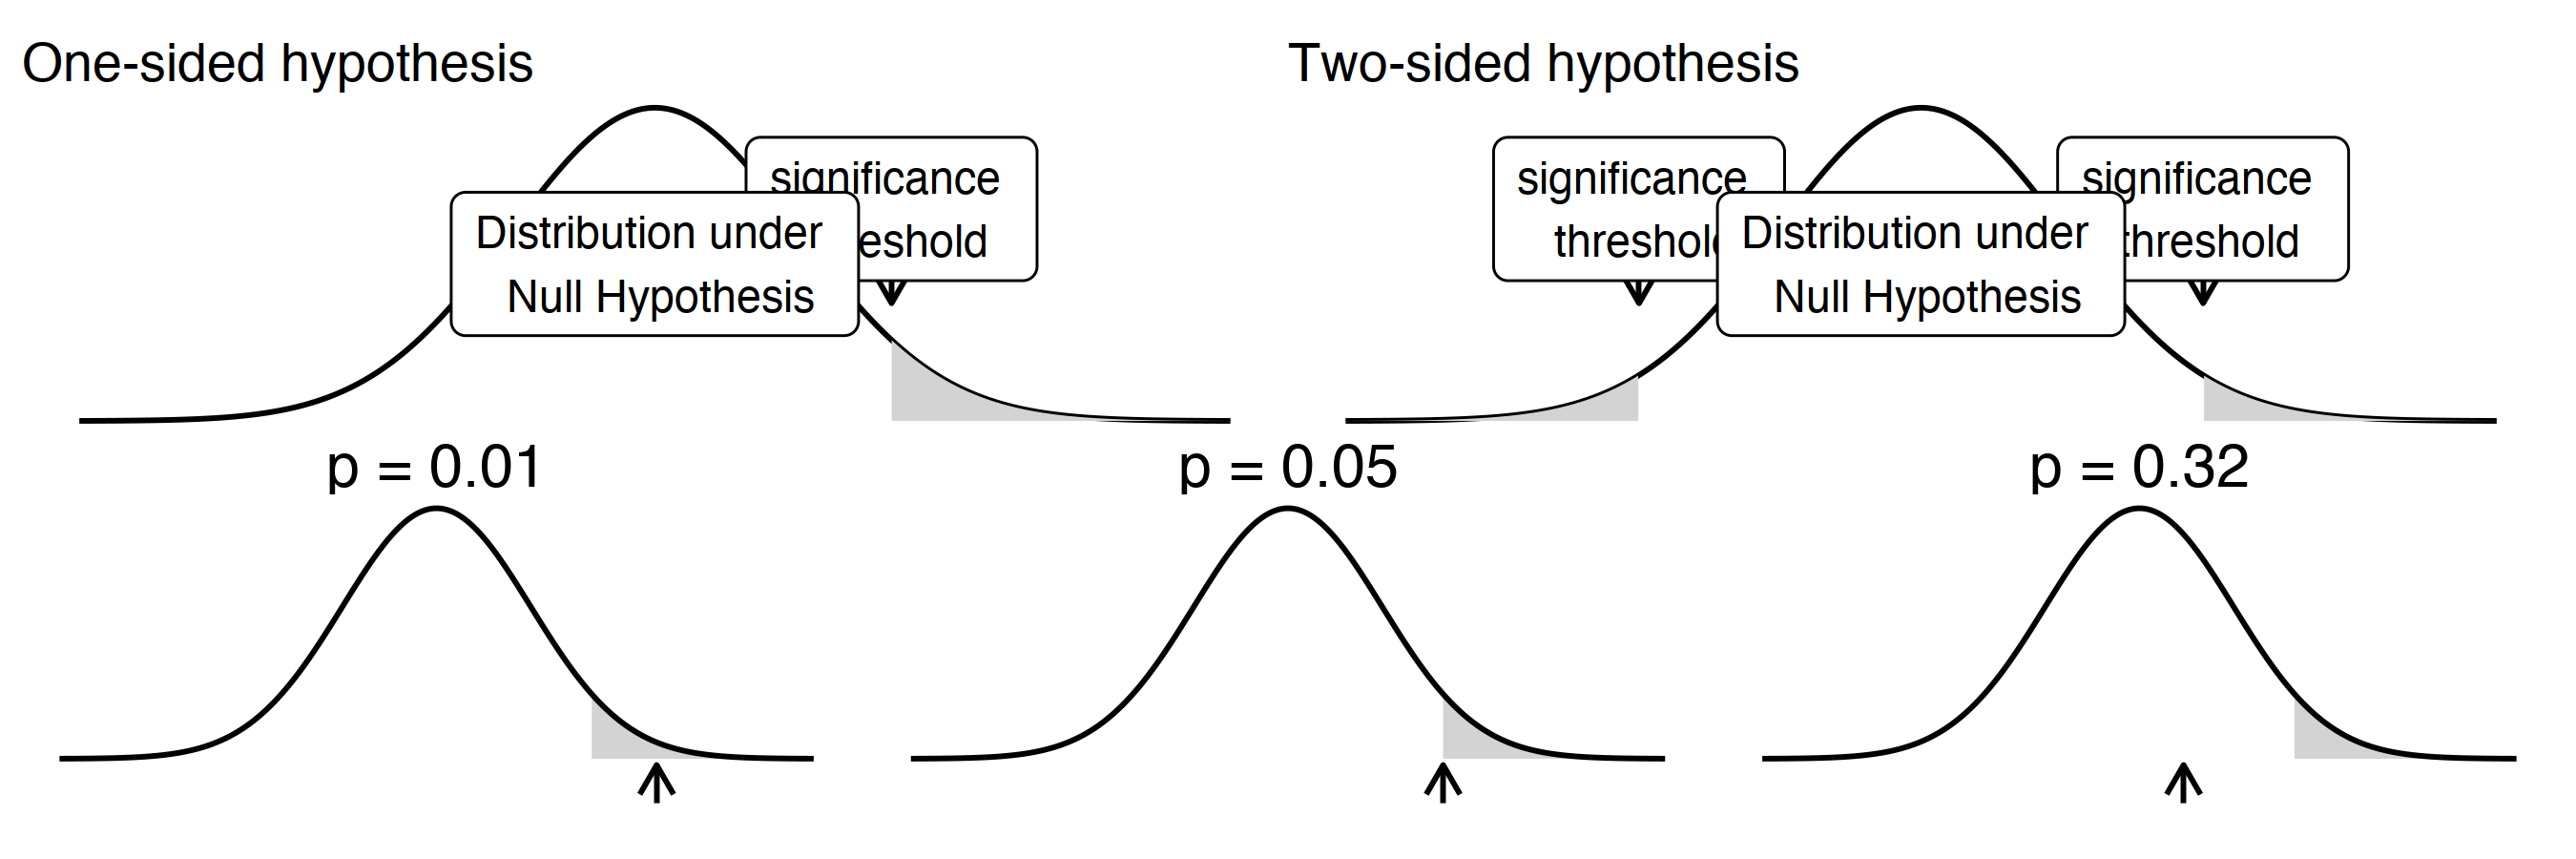
\includegraphics[width=0.8\textwidth]{figures/hypothesis-1} 

}

\caption{Frequentists make binary decisions based on hypothesis tests. Assuming the null distribution, the null hypothesis is rejected if the observed estimand is extreme.}\label{fig:hypothesis}
\end{figure}

Null hypothesis testing is very weird.
It's like answering the question around two corners.
Let's say a researcher wants to prove that a drug prevents migraines.
They test the drug because they expect it to work, so the hypothesis they assume to be true is that patients that take the drug have fewer migraines.
But the null hypothesis is formulated the other way around:
The null hypothesis assumes that the drug has no effect.
Suddenly the goal of the researcher becomes to show that the null hypothesis is false, rather than showing that their hypothesis is correct.
The problem with statistical models is: We can't prove that they are true because our assumptions are not testable.
With frequentist inference, however, we can tell how likely a model result is under a given hypothesis and given the data.
That's why hypothesis tests work by rejection.
The \protect\hyperlink{likelihoodism}{likelihoodist mindset} navigates this issue:
two statistical models are compared in terms of the evidence through the likelihood.

Null hypothesis tests are even more troublesome.

\begin{itemize}
\tightlist
\item
  The choice of the null hypothesis is arbitrary.
\item
  If the null hypothesis is accepted, it's not evidence that it's true. It just means that the data that were observed are not in conflict with the null hypothesis. But there is still an infinite number of models that could have produced the same results.
\item
  If the null hypothesis is rejected, it doesn't mean that the hypothesis of interest is true.
\item
  A significant result doesn't mean that the deviation from the null hypothesis is relevant. The drug has a significant effect on the disease progression? The difference might be too small to be relevant.
\item
  Especially the larger the data sample, the more likely the null hypothesis is rejected, because the tiniest differences to the null hypothesis are enough to produce significant results when \(n\) becomes large.
\end{itemize}

\hypertarget{confidence-intervals}{%
\section{Confidence Intervals}\label{confidence-intervals}}

Frequentists use confidence intervals as an alternative to statistical tests.
Hypothesis tests and confidence intervals ultimately lead to the same decisions, but confidence intervals are more informative.
Many statisticians prefer confidence intervals over mere p-values.

Remember that estimators, such as model parameters, are random variables?
That means that estimators have probability distributions.
A confidence interval describes where the mass of that distribution lies.
The interval consists of the estimator, and the lower and upper bounds for the mass of the distribution.
The modeler decides the percentage of the distribution in the confidence interval through the \(\alpha\)-level.
If \(\alpha = 0.05\), then we get a 95\%-confidence interval.
The construction of the confidence interval depends on the probability distribution we have derived for the quantity of interest (coefficient, mean estimate, \ldots).

How are the confidence intervals to be interpreted?
Well, in a frequentist manner, of course!
The ``true'' parameter value is fixed, so it's not a random variable.
To say that the true parameter is in the confidence interval with a 95\% probability would be false.
The true parameter is either in the interval or it's not, we just don't know.
The confidence itself is a random variable since it's derived from data and therefore from other random variables.
So the interpretation of a 95\% confidence interval is:
If we were to repeat the analysis many times, the confidence interval would cover the true value of the quantity of interest 95\% of the time.
Only given that the model assumptions are correct.
As you can see, this is a very frequentist point of view: the confidence interval is interpreted in the context of repeated experiments.

\begin{figure}

{\centering 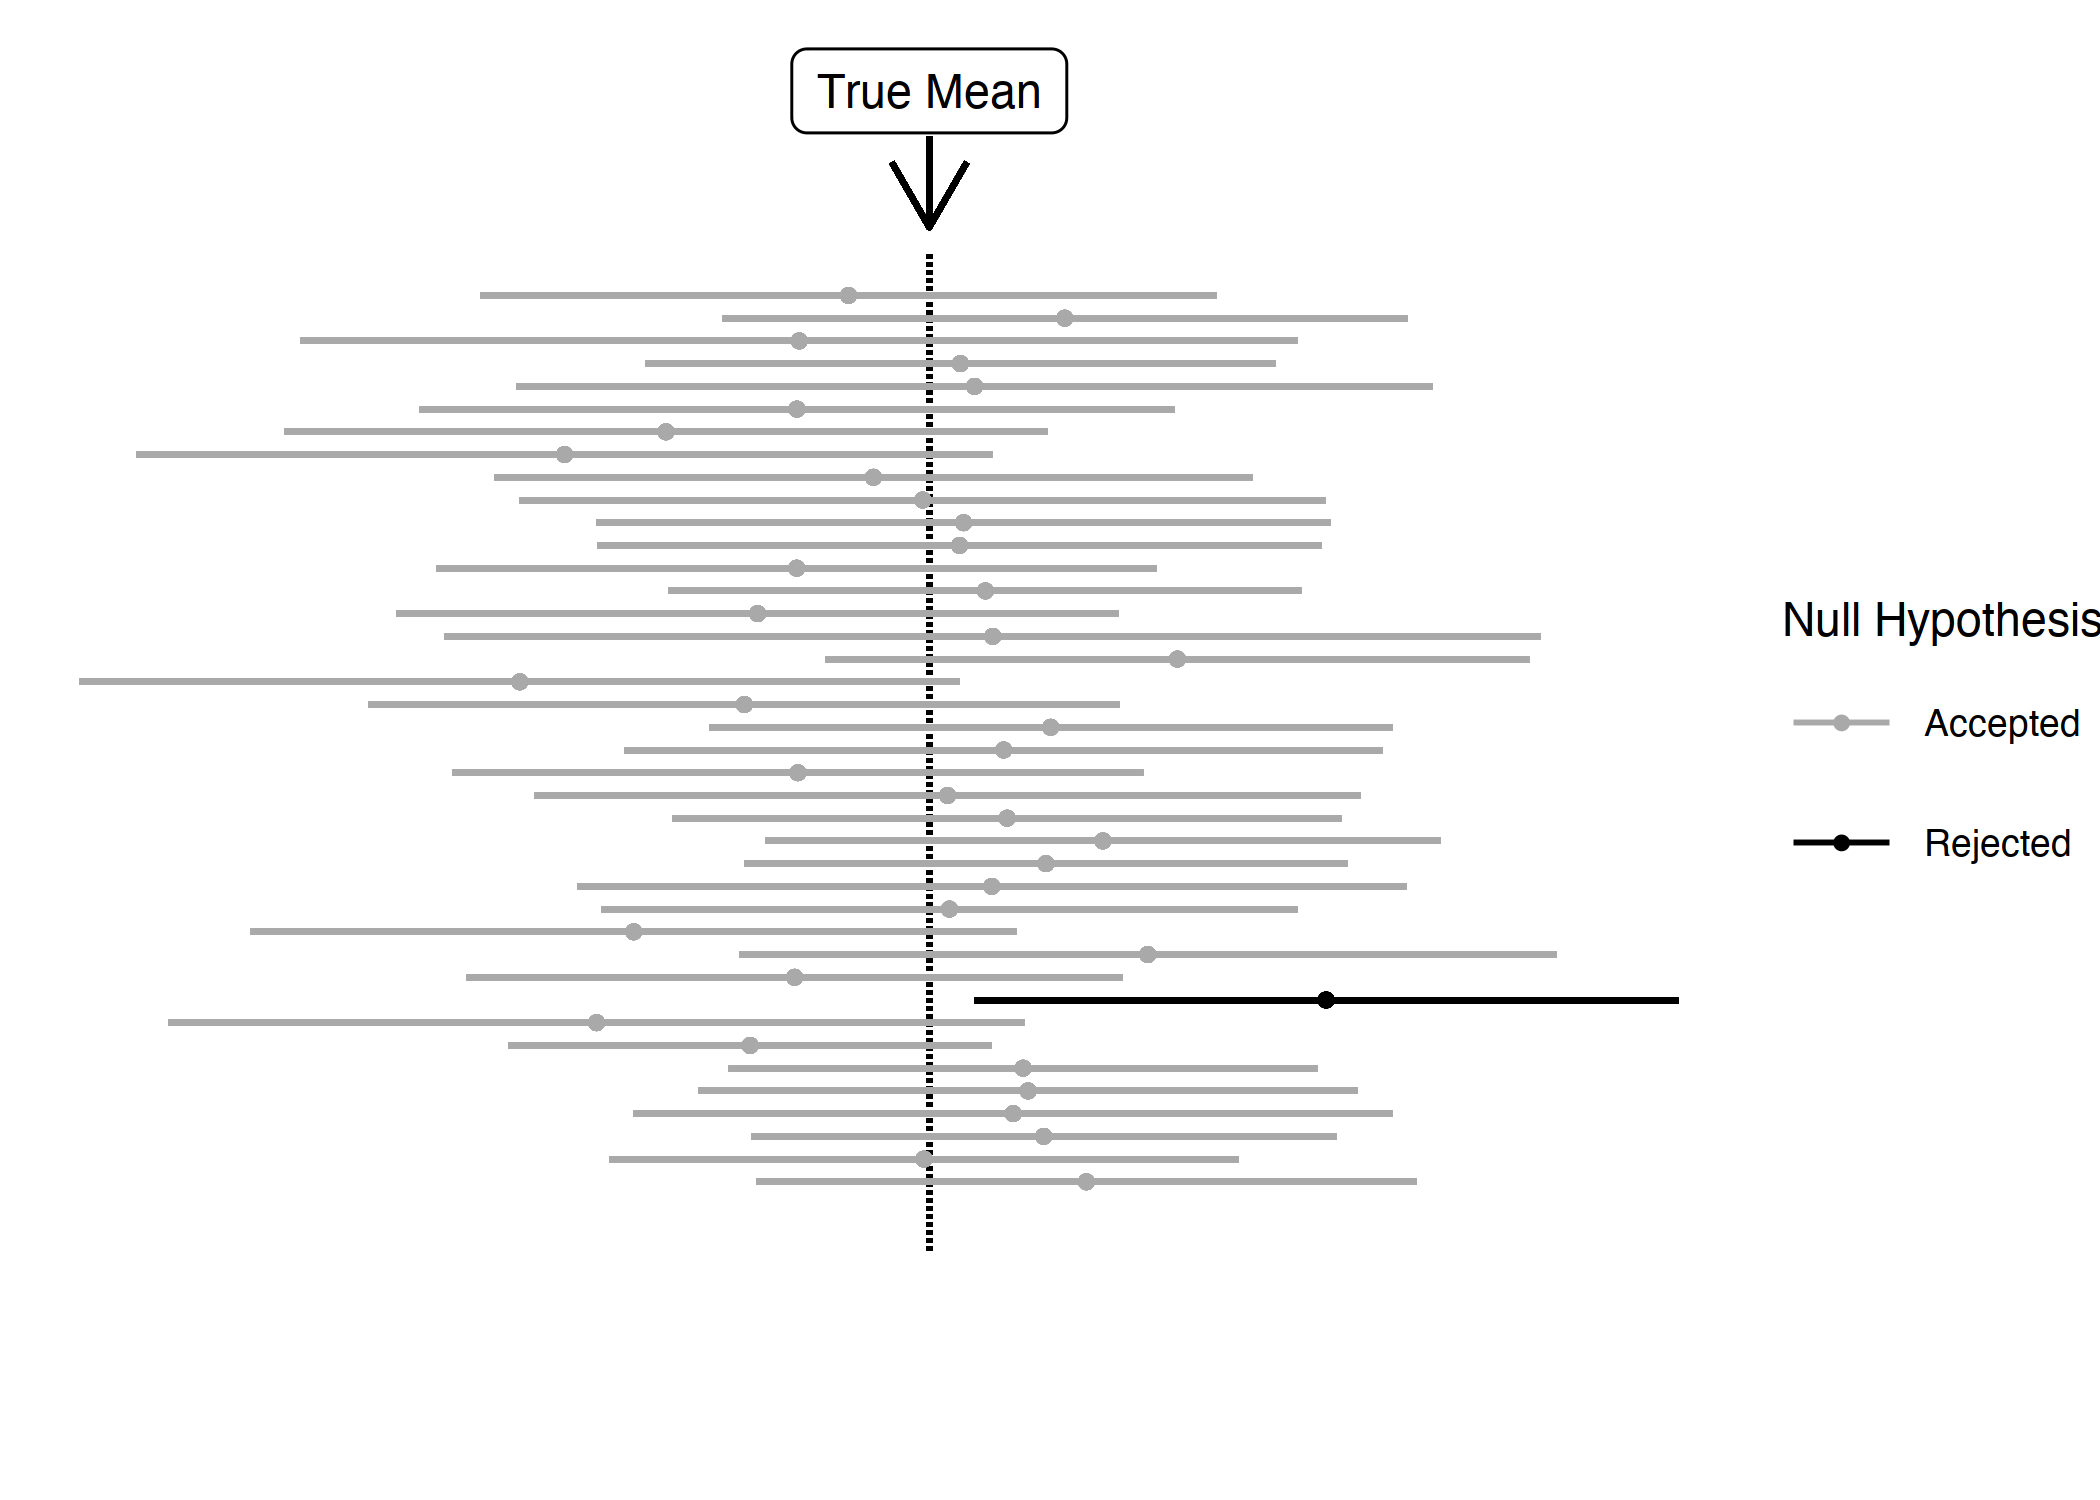
\includegraphics[width=0.8\textwidth]{figures/ci-1} 

}

\caption{100 95\% confidence intervals and the true value.}\label{fig:ci}
\end{figure}

\hypertarget{strengths-1}{%
\section{Strengths}\label{strengths-1}}

\begin{itemize}
\tightlist
\item
  Once you understand frequentist inference, you have the key to understanding most modern research findings. I studied statistics and can now quickly grasp many research papers. For example, to figure out whether I should have knee surgery for my torn meniscus, I read papers comparing knee surgery and physiotherapy alone. All of those papers used frequentist methods, and although I didn't understand everything, I was able to quickly get an idea of their analyses and results.
\item
  Frequentist methods are generally faster to compute than methods from \protect\hyperlink{bayesian-inference}{Bayesian inference} or \protect\hyperlink{supervised-ml}{machine learning}.
\item
  Compared to \protect\hyperlink{bayesian-inference}{Bayesianism}, no prior information about the parameters is required. This makes frequentism more objective.
\item
  Frequentism allows binary decisions (accept/reject hypothesis). This simplicity is one of the reasons why frequentism is popular for both scientific publications and business decisions.
\item
  Frequentism has all advantages of \protect\hyperlink{statistical-modeling}{statistical models} in general: a solid theoretical foundation and an appreciation of the data-generating process.
\item
  When the underlying process is a long-run, repeated experiment, frequentist inference shines. Casino games, model benchmarks, \ldots{}
\item
  The scientific method requires that scientific experiments be repeatable. The frequentist idea that truth lies in long-run frequencies of experiments is therefore well compatible with a core idea of science.
\end{itemize}

\hypertarget{limitations-1}{%
\section{Limitations}\label{limitations-1}}

\begin{itemize}
\tightlist
\item
  Frequentism makes it easy to \textbf{over-simplify questions} into yes/no-questions. Reducing models to binary decisions obscures critical model assumptions and the difficult trade-offs that had to be made for the analysis.
\item
  Focusing on p-values encourages \textbf{p-hacking}: the either conscious or unconscious search for ``positive'' results. Guided by the lure of a significant result, researchers and data scientists may play around with their analysis until the p-value in question is small enough. With \(\alpha\)-level of 0.05, 1 in 20 null hypotheses are falsely rejected. P-hacking increases this percentage of false positive findings.
\item
  Similarly, if the analysis is exploratory rather than hypothesis-driven, a naive frequentist approach may produce many false positive findings. Look again at figure \ref{fig:ci}: Imagine these were confidence intervals for different variables. Again, for \(\alpha = 0.05\), we would expect 1 in 20 hypothesis tests to yield false positives. Now imagine a data scientist testing hundreds of hypothesis tests. This problem is called the multiple testing problem. There are solutions, but they are not always used and multiple testing can be very subtle.
\item
  The frequentist interpretation of probability is very awkward when it comes to confidence intervals and p-values. They are commonly misinterpreted. Arguably, frequentist confidence intervals are not what practitioners want. \protect\hyperlink{bayesian-inference}{Bayesian} credibility intervals are more aligned with the natural interpretation of uncertainty.
\item
  Frequentist analysis depends not only on the data, but also on the experimental design. This is a violation of the likelihood principle that says that all information about the data must be contained in the likelihood, see also the example in the \protect\hyperlink{likelihoodism}{Likelihoodism} chapter.
\item
  Frequentist probability can fail in the simplest scenarios: Imagine you are modeling the probability of rain in August. The data only has 20 August days, all of which are without rain. The frequentist answer is that there is absolutely no chance that it will ever rain in August. The frequentist recommendation is that to collect more data if we want a better answer. \protect\hyperlink{bayesian-inference}{Bayesianism} offers a solution to involve prior information for such estimates.
\item
  There is an ``off-the-shelf''-mentality among users of frequentist inference. Instead of carefully adapting a probability model to the data, an off-the-shelf statistical test or statistical model is chosen. The choice is based on just a few properties of the data. For example, there are popular flow charts of choosing an appropriate statistical test.
\item
  Frequentist statistics says nothing about causality except that ``correlation does not imply causation''.
\item
  Weird interpretation of probability: Often it does not make any sense to interpret every probability with imagined experiments. For example, the probability for a party to get the majority vote in an election requires to imagine multiple elections, yet under the same circumstances, like same year, same candidates, and so on.
\end{itemize}

\hypertarget{bayesian-inference}{%
\chapter{Bayesian Inference}\label{bayesian-inference}}

\begin{itemize}
\tightlist
\item
  Probability is a degree of belief, and learning from data means updating belief.
\item
  Model parameters are random variables with prior and posterior distributions.
\item
  A \protect\hyperlink{statistical-modeling}{statistical modeling mindset} with \protect\hyperlink{frequentist-inference}{frequentism} and \protect\hyperlink{likelihoodism}{likelihoodism} as alternatives.
\end{itemize}

While frequentists analyze data to answer the question ``What should I do?'', Bayesians analyze data to answer ``What should I believe?''.

If you haven't read the chapter on \protect\hyperlink{statistical-modeling}{Statistical Modeling}, I recommend that you do so first, since Bayesian inference is easier to understand if you have a good understanding of statistical inference.
Bayesian inference is based on probability distributions, interpreting parameters, and learning from data through the likelihood.
The twist: distribution parameters are also random variables.
Random variables that have a prior distribution.
Prior means before encountering the data.
Learning about the parameters means updating the prior probabilities to the posterior probabilities.

In Bayesian statistics, probability can be interpreted as the plausibility of an event or our belief about it.
That's different from the more objective interpretation of probability in \protect\hyperlink{frequentist-inference}{frequentist inference}.
In Bayesian inference, it's not necessary to imagine repeated experiments.
One can even apply Bayesian inference to a single data point.
This is not possible with frequentist inference.
A Bayesian model even works without data, by just using the prior distributions. \footnote{This is called the prior predictive simulation and is used to check that the chosen priors produce reasonable data. The modeler simulates by first sampling parameters from the priors and using those parameters to generate data. Repeating this several times results in a distribution of data.}

\hypertarget{bayes-theorem}{%
\section{Bayes Theorem}\label{bayes-theorem}}

Bayesians want to learn the distribution of the model parameters from the data: \(P(\theta | X)\).
\(P(\theta | X)\) is a strange way of looking at the probabilities involved.
The data-generating process generates data as a function of the parameters: \(P(X | \theta)\).
So Bayesians look for the inverse of what the DGP would naturally do.

To make \(P(\theta|X)\) computable, Bayesians use a trick that earned them their name: the Bayes' theorem.
Bayes' theorem can be used to invert the conditional probability:

\[\underbrace{P(\theta|X)}_{\text{posterior}} = \frac{\overbrace{P(X | \theta)}^{\text{likelihood}} \cdot  \overbrace{P(\theta)}^{\text{prior}}}{\underbrace{P(X)}_{\text{evidence}}}\]

\(P(\theta)\), also called prior, is the probability distribution of \(\theta\) before we have collected any data.
The probability distribution is updated by multiplying the prior by the data likelihood \(P(X | \theta)\). \footnote{In the Bayesian mindset \(\theta\) is a random variable, so the notation can be confusing: \(P(X | \theta)\) refers to the likelihood function. The same function that we used in frequentist inference. But in the frequentist inference, we might write \(P(\theta | X)\) to emphasize that \(\theta\) is the input that varies. But this notation refers to the posterior in Bayesian statistics, so we write \(P(X | \theta)\).}
This product is scaled by the probability of the data \(P(X)\), also called evidence.
The result is the posterior probability distribution, an updated belief about the parameters \(\theta\).

Bayes' theorem is a generally useful equation for working with probabilities, but we focus on its use for Bayesian inference.
The theorem is not just a simple rearrangement of probabilities, but a powerful mental model: Bayesian updating.
Remember that the data likelihood is the product of the likelihoods for each data point:
\$\(P(X | \theta) = \prod_{i=1}^n P(X^{(i)} | \theta)\).
Here, \(X^{(i)}\) is the vector of random variables of the i-th outcome.
For example, in a drug trial, the variables \$X\^{}\{(i)\} could belong to the i-th (not yet observed) patient and include pain level, blood pressure and iron level.
Plugging this version of the likelihood into Bayes' theorem, we can see how it relates to updating ones belief with new data.
For simplicity, I have removed the evidence \(P(X)\) which only serves as a normalization so we can interpret the results as probability:

\begin{eqnarray}
P(\theta|X) & \propto  & P(X | \theta) \cdot  P(\theta) \\ 
            & =        & P(\theta) \cdot \prod_{i=1}^n P(\theta, X^{i}) \\
            & =        & P(\theta) \cdot P_1 \cdot \ldots \cdot P_p,
\end{eqnarray}

where \(P_i = P(X^{(i)} | \theta)\).
Even with just one data point, we can update our belief about the parameters!
And each time, this posterior then becomes -- in a sense -- the prior for the next update.
The posterior distribution is the product of prior and likelihood (Figure \ref{fig:bayesian}).

\begin{figure}

{\centering 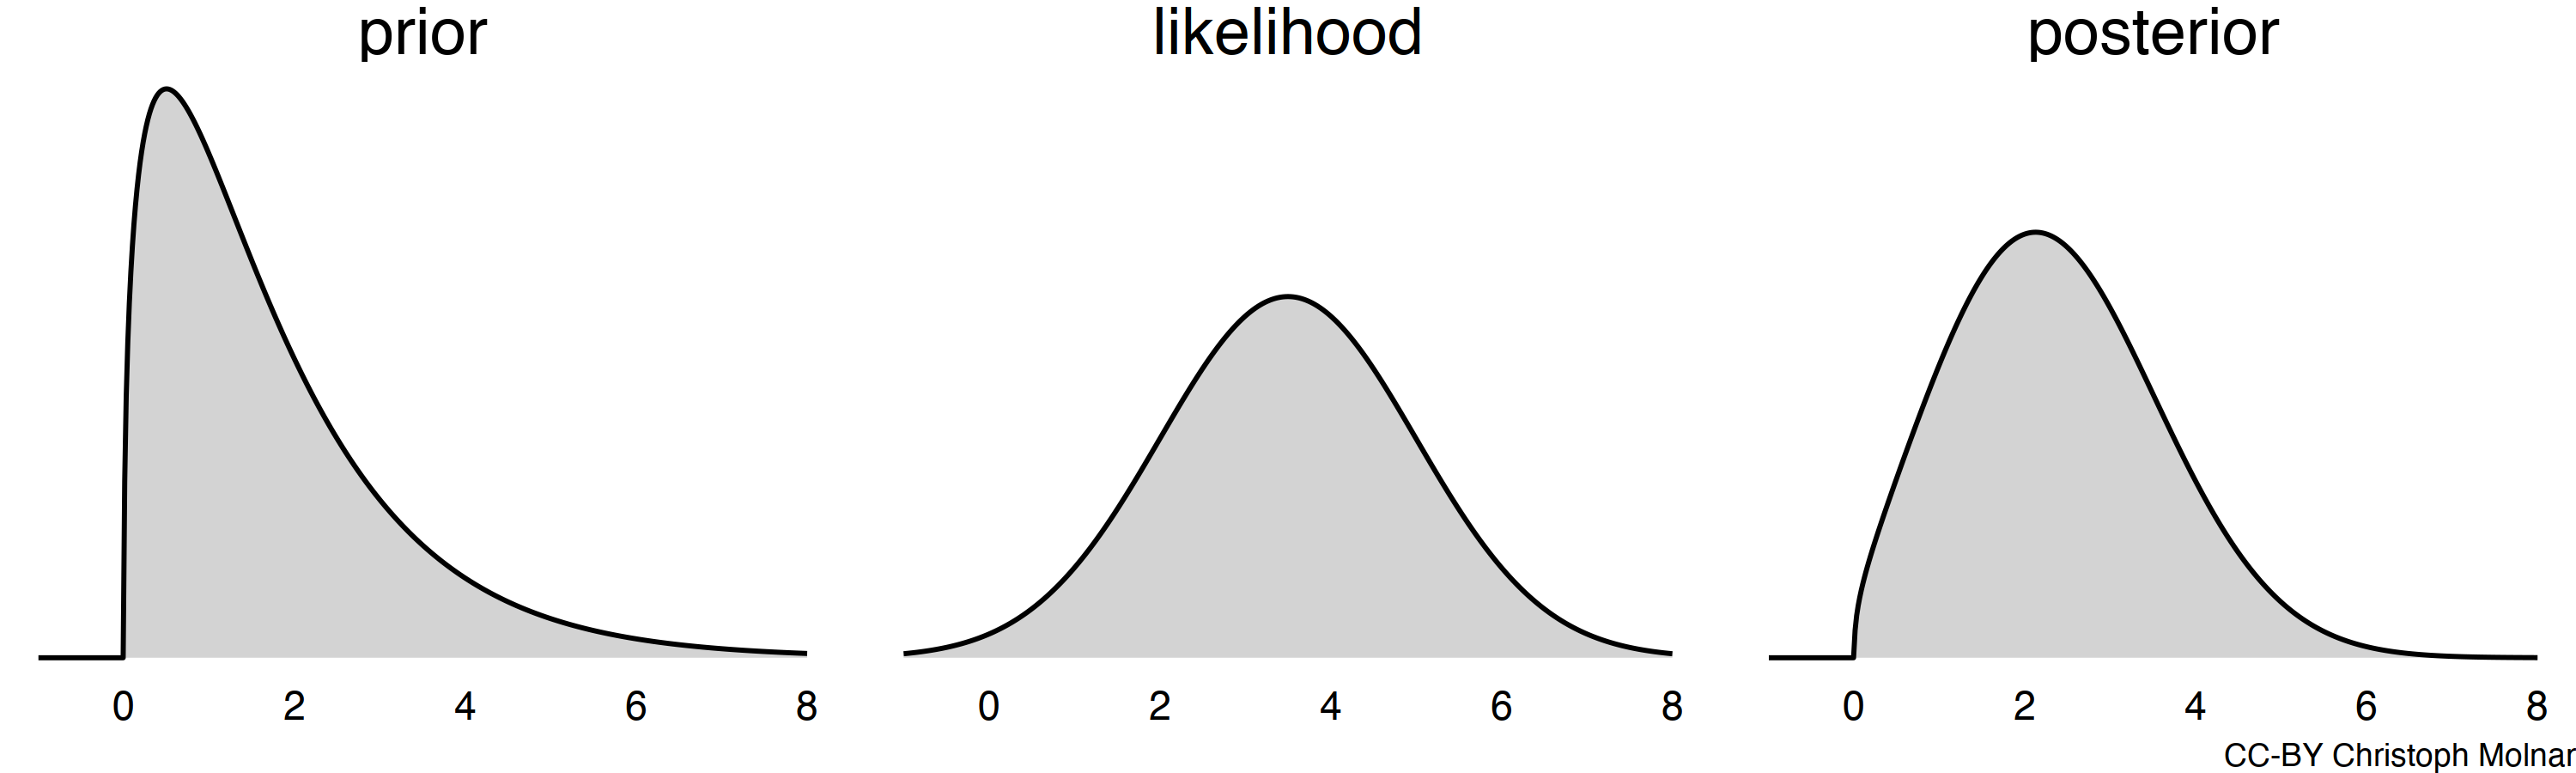
\includegraphics[width=0.8\textwidth]{figures/bayesian-1} 

}

\caption{The posterior distribution (right) is the scaled product of prior and likelihood: prior $\times$ likelihood $\propto$ posterior.}\label{fig:bayesian}
\end{figure}

Next, let's explore the individual terms of Bayes' theorem, so that we can update our own beliefs about Bayesian inference.

\hypertarget{prior-probability}{%
\section{Prior Probability}\label{prior-probability}}

Bayesians assume that model or distribution parameters a prior probability distribution \(P(\theta)\). \footnote{When I was learning about Bayesian inference, one of my first question was: do the parameters of the priori distributions have priori distributions themselves? Where does it end? The answer: Bayesian stop after one level of priori distributions and don't go full inception.}
Let's say we randomly pick a person and want to know how many hours per day they usually work.
The number of hours worked per day, the random variable of interest, follows a probability distribution.
For example, the number of hours worked might follow a Gaussian distribution.
Bayesians assume that mean and variance of this Gaussian distribution are random variables.

How do priors make sense?
How can Bayesians know the distribution of parameters \emph{before} observing any data?
Priors are a consequence of saying that parameters are random variables, and a technical requirement for working with the Bayes' theorem.
But how can we know anything about the parameters before we see the data?

\hypertarget{picking-a-prior}{%
\subsection*{Picking a Prior}\label{picking-a-prior}}


The first consideration in choosing a prior is the \emph{space} the parameter is in.
Is the parameter the mean of a continuous distribution?
If so, it makes sense for the parameter to follow a continuous distribution as well, such as a Gaussian distribution.
Maybe the mean of the data distribution has to be positive.
Then the prior distribution should contain only positive values (meaning the probability for negative values should be zero), for example, the Gamma distribution.
Furthermore, expert knowledge can be used to choose the prior.
Maybe we know from other experiments that the mean parameter should be around 1.
So we could assume a Gaussian distribution for \(\theta\): \(\theta \sim N(1, 1)\).
In the case where the data follow a Binomial distribution, the Beta distribution is a good prior (see Figure \ref{fig:priors}).
Depending on what the modelers believes about the success probability parameter \(p\) of the Binomial distribution, they might choose different parameterizations of the Beta distribution.
Maybe the modeler believes that the parameter must be symmetrically distributed around 0.5.
Or maybe the parameter is lower, around 0.25?
Another Beta prior might put emphasis on \(p\) being 1.
It's even possible to have a prior that that places the greatest probability symmetrically on 0 and 1.

Without expert knowledge about the parameter, the modeler can use ``uninformative'' or ``objective'' priors\textsuperscript{\protect\hyperlink{ref-yang1996catalog}{7}}.
Uninformative priors often produce results similar to those of frequentist inference (for example for confidence/credible intervals).
Another factor influencing the choice of prior is mathematical convenience.
Conjugate priors are convenient choices.
Conjugate priors remain in the same family of distributions when multiplied by the right likelihood functions.
A Beta prior distribution multiplied by a Bernoulli likelihood, in turn, produces a Beta posterior distribution.

Although there are all these different strategies for choosing a prior, even ``objective'' ones, the choice remains subjective.
And this subjective choice of prior is why many frequentists reject Bayesian inference.
While the prior can be seen as a bug, it can also be seen as a feature.
Thanks to the prior, Bayesian modeling is very flexible.
The prior can be used to constrain and regularize model parameters, especially when data are scarce;
the prior can encode results from other experiments and expert knowledge;
the prior allows a natural handling of measurement errors and missing data.

To obtain the posterior distribution of the parameters -- the ultimate goal of Bayesian inference -- we need to update the prior using data, or rather, the likelihood function.

\begin{figure}

{\centering 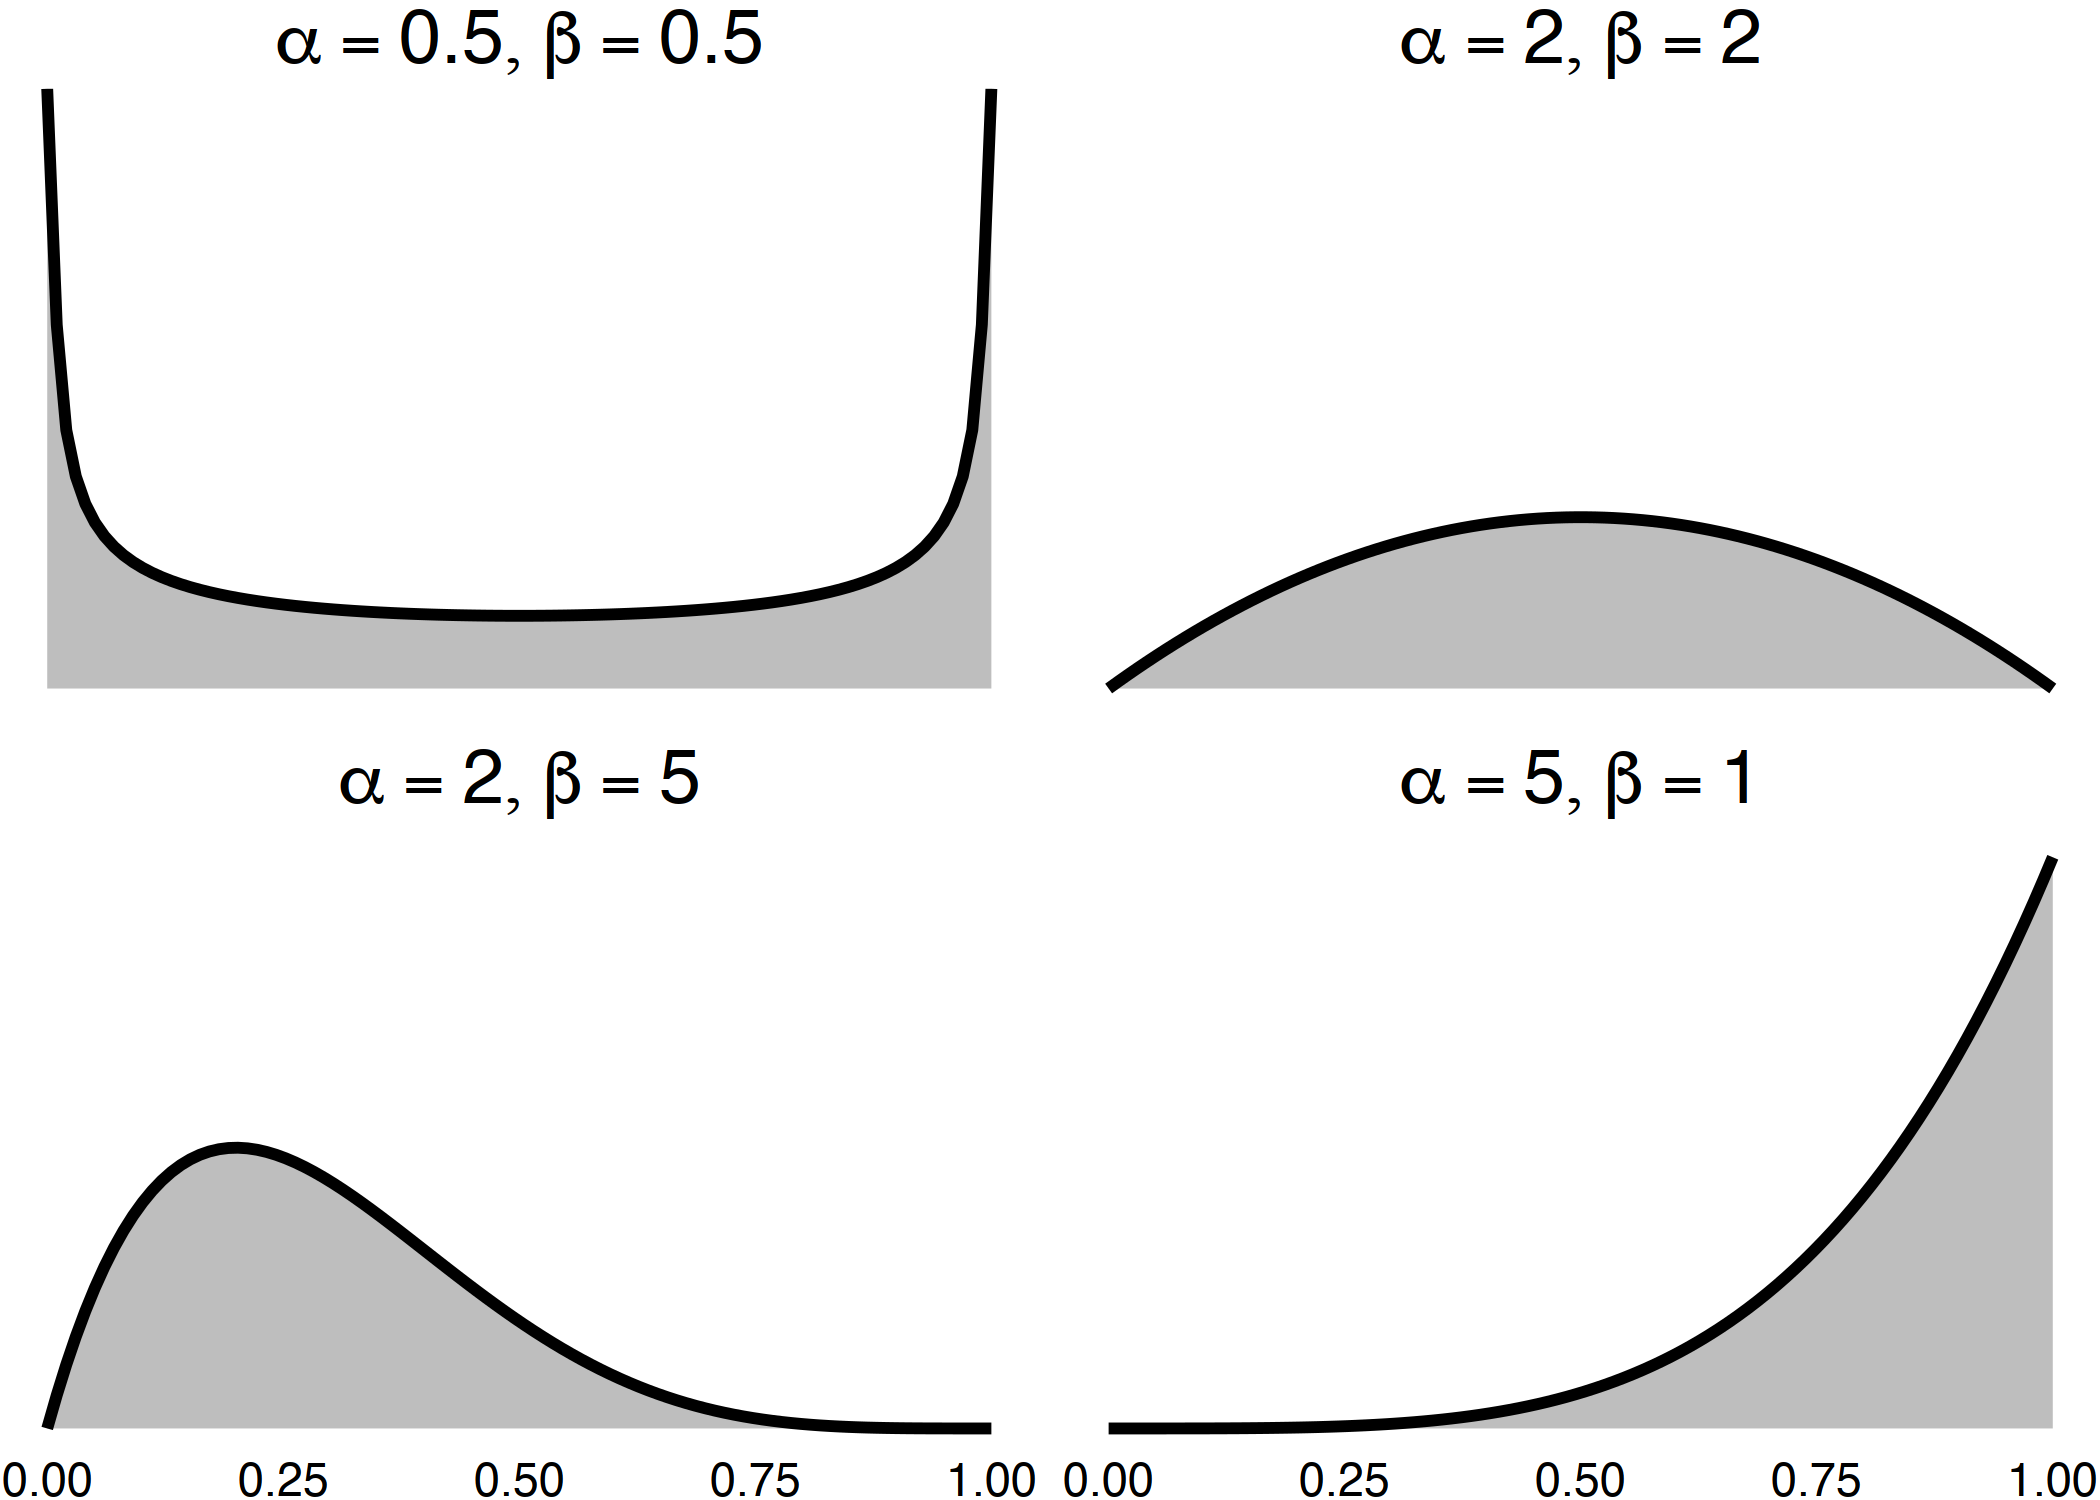
\includegraphics[width=0.8\textwidth]{figures/priors-1} 

}

\caption{Various Beta prior distributions for the success probability p in a Binomial distribution. The parameters $\alpha$ and $\beta$ influence the shape of the Beta prior.}\label{fig:priors}
\end{figure}

\hypertarget{likelihood}{%
\section{Likelihood}\label{likelihood}}

If you have read the chapter \protect\hyperlink{statistical-modeling}{Statistical Modeling}, you should be familiar with the likelihood function \(P(\theta, X)\).
The likelihood is equivalent to the probability function of the data.
Only that the focus is switched: the likelihood is a function of the parameters, while the probability is a function of the data.

The Bayesian makes an assumption about how the data are distributed and forms the likelihood function.
This is no different than \protect\hyperlink{frequentism}{frequentism} and \protect\hyperlink{likelihoodism}{likelihoodism}.
But for Bayesians, the likelihood is just one part of the equation.

With all the comparisons between frequentist inference and Bayesian inference, it's easy to forget that both approaches are quite similar.
Comparisons between the two mindsets often focus on the (lack of) prior distribution.
This overlooks the fact that both frequentist and Bayesian inference use the likelihood at the core of their models.
Especially in cases with a lot of data, both approaches produce similar results.
That's because the more data are available for the model, the less impact the prior has on the Bayesian results.

Let's now turn to the last part of the equation: the evidence \(P(X)\).

\hypertarget{evidence}{%
\section{Evidence}\label{evidence}}

The evidence is the marginalized probability of the data.
Marginalized means that the probability of the data is integrated over all possible parameter values: \(P(X) = \int_{\Theta} P(X|\theta) P(\theta) d\theta\), where \(\Theta\) are all possible parameter values.
Because of this marginalization, \(P(X)\) is no longer a function of the parameters \(\theta\).
\(P(X)\) is just a constant factor in terms of maximizing the posterior probability
Constant factors don't change \emph{where} the maximum is, just how large it is.
In search of the maximum, the evidence \(P(X)\) can be ignored.
For this reason, the posterior probability is often expressed as proportional to the numerator:

\[\underbrace{P(\theta|D)}_{\text{posterior}} \propto \overbrace{P(D | \theta)}^{\text{likelihood}} \cdot  \underbrace{P(\theta)}_{\text{prior}}\]

Just one problem: When throwing away \(P(X)\), the posterior probability is not a probability at all, because it doesn't integrate to 1, but to \(P(X)\).
How can this problem be solved?

\hypertarget{posterior-probability-estimation}{%
\section{Posterior Probability Estimation}\label{posterior-probability-estimation}}

The goal of the Bayesian modelers is to estimate the posterior distributions of the parameters.
Once the modelers have the posteriors, they can interpret them, make predictions, and draw conclusions about the world.

But how is the posterior estimated?
In the ideal case, the posterior can be written down as a simple formula.
But that's only possible for certain combinations of prior and likelihood, for example when conjugate priors are used.
For many Bayesian models it's impossible to obtain a closed form for the posterior.
The main problem is that \(P(X)\) may not be computable.

\hypertarget{sample-from-the-posterior-with-mcmc}{%
\subsection*{Sample From the Posterior with MCMC}\label{sample-from-the-posterior-with-mcmc}}


The good news: We don't have to compute the posterior probability.
We can sample from it.
Approaches such as Markov Chain Monte Carlo (MCMC) and derivations thereof are used to generate samples from the posterior distribution.

The rough idea of MCMC and similar approaches is as follows:

\begin{itemize}
\tightlist
\item
  Start with some initial values for the parameters \(\theta\).
\item
  Repeat the following steps until a stopping criterion is reached (like pre-determined number of samples):

  \begin{enumerate}
  \def\labelenumi{\arabic{enumi}.}
  \tightlist
  \item
    Propose new parameter values. Proposals are based on a proposal function receives as input the previous parameters.
  \item
    Accept or reject the new values, based on an acceptance function. The acceptance function depends on the prior and the likelihood, but not on the evidence.
  \item
    If the new parameter are accepted, continue with these new values.
  \end{enumerate}
\end{itemize}

A run of MCMC produces a ``chain'' of samples from the posterior distribution.
MCMC can be repeated to produce multiple chains.

MCMC has many variants such as Gibbs sampling and the Metropolis-Hastings algorithm.
Each variant differs in proposal and acceptance functions or other algorithmic steps.

MCMC produces a random walk through the posterior distribution of the parameters.
Regions where the parameters have a high probability are also ``visited'' with a higher probability.
The samples can be seen as samples from the posterior.
But first, some cleaning up needs to happen:
Since MCMC has to start somewhere, it's possible that the first samples will be from parameter regions with low probability.
So the first 1000 or so samples are ``burned'', meaning they are not used for estimating the posterior.
Another problem is autocorrelation within the chain:
Samples that occur one after the other are correlated since the proposal function usually proposes new parameters that are close to the previous values.
So the chain is sampled at different points to ensure that there are enough MCMC steps between two samples to make them independent.

MCMC sampling can be complex and can take some time to compute.
Fortunately, most probabilistic software runs MCMC automatically.
But this can take time.
More time than fitting a frequentist model would take.
A shorter alternative is variational inference.\textsuperscript{\protect\hyperlink{ref-blei2017variational}{8}}
But while MCMC delivers approximately exact estimates of the posterior probability, variational inference is more of a heuristic.

Frequentists have their parameter estimates.
Bayesians have \ldots{} samples from the posterior distribution?
That's not the end of the story.
There are two more steps required to get from posterior samples to insights: turning the samples to a distribution and (optionally) summarizing the distribution.

\hypertarget{summarizing-the-posterior-samples}{%
\section{Summarizing the Posterior Samples}\label{summarizing-the-posterior-samples}}

The posterior samples can be visualized with a histogram or a density estimator for a smoother looking curve.
Visualizing the entire posterior is the most informative way of reporting the Bayesian results.

People love numbers and tables.
The fewer and simpler, the better.
You won't get your manager to understand posterior distributions.
They demand simple answers!
So, let's simplify the posterior.
There's advice about not summarizing the posterior\textsuperscript{\protect\hyperlink{ref-tiao1973some}{9}}, but people do it anyways.
Summaries of the posterior can be points or intervals.
Intervals can be defined via fixed boundaries or fixed probability mass.
Some examples:

\begin{itemize}
\tightlist
\item
  Point estimate: The parameter value with the highest posterior probability.
\item
  Interval with fixed boundaries: The interval from 10 to infinity indicates the probability that the parameter is greater than 10.
\item
  Interval with fixed probability mass: The shortest interval containing 50\% of the posterior probability mass. Or the interval that ranges from the 2.5\% quantile to the 97.5\% quantile ( called the 95\% credible interval).
\end{itemize}

\begin{figure}

{\centering 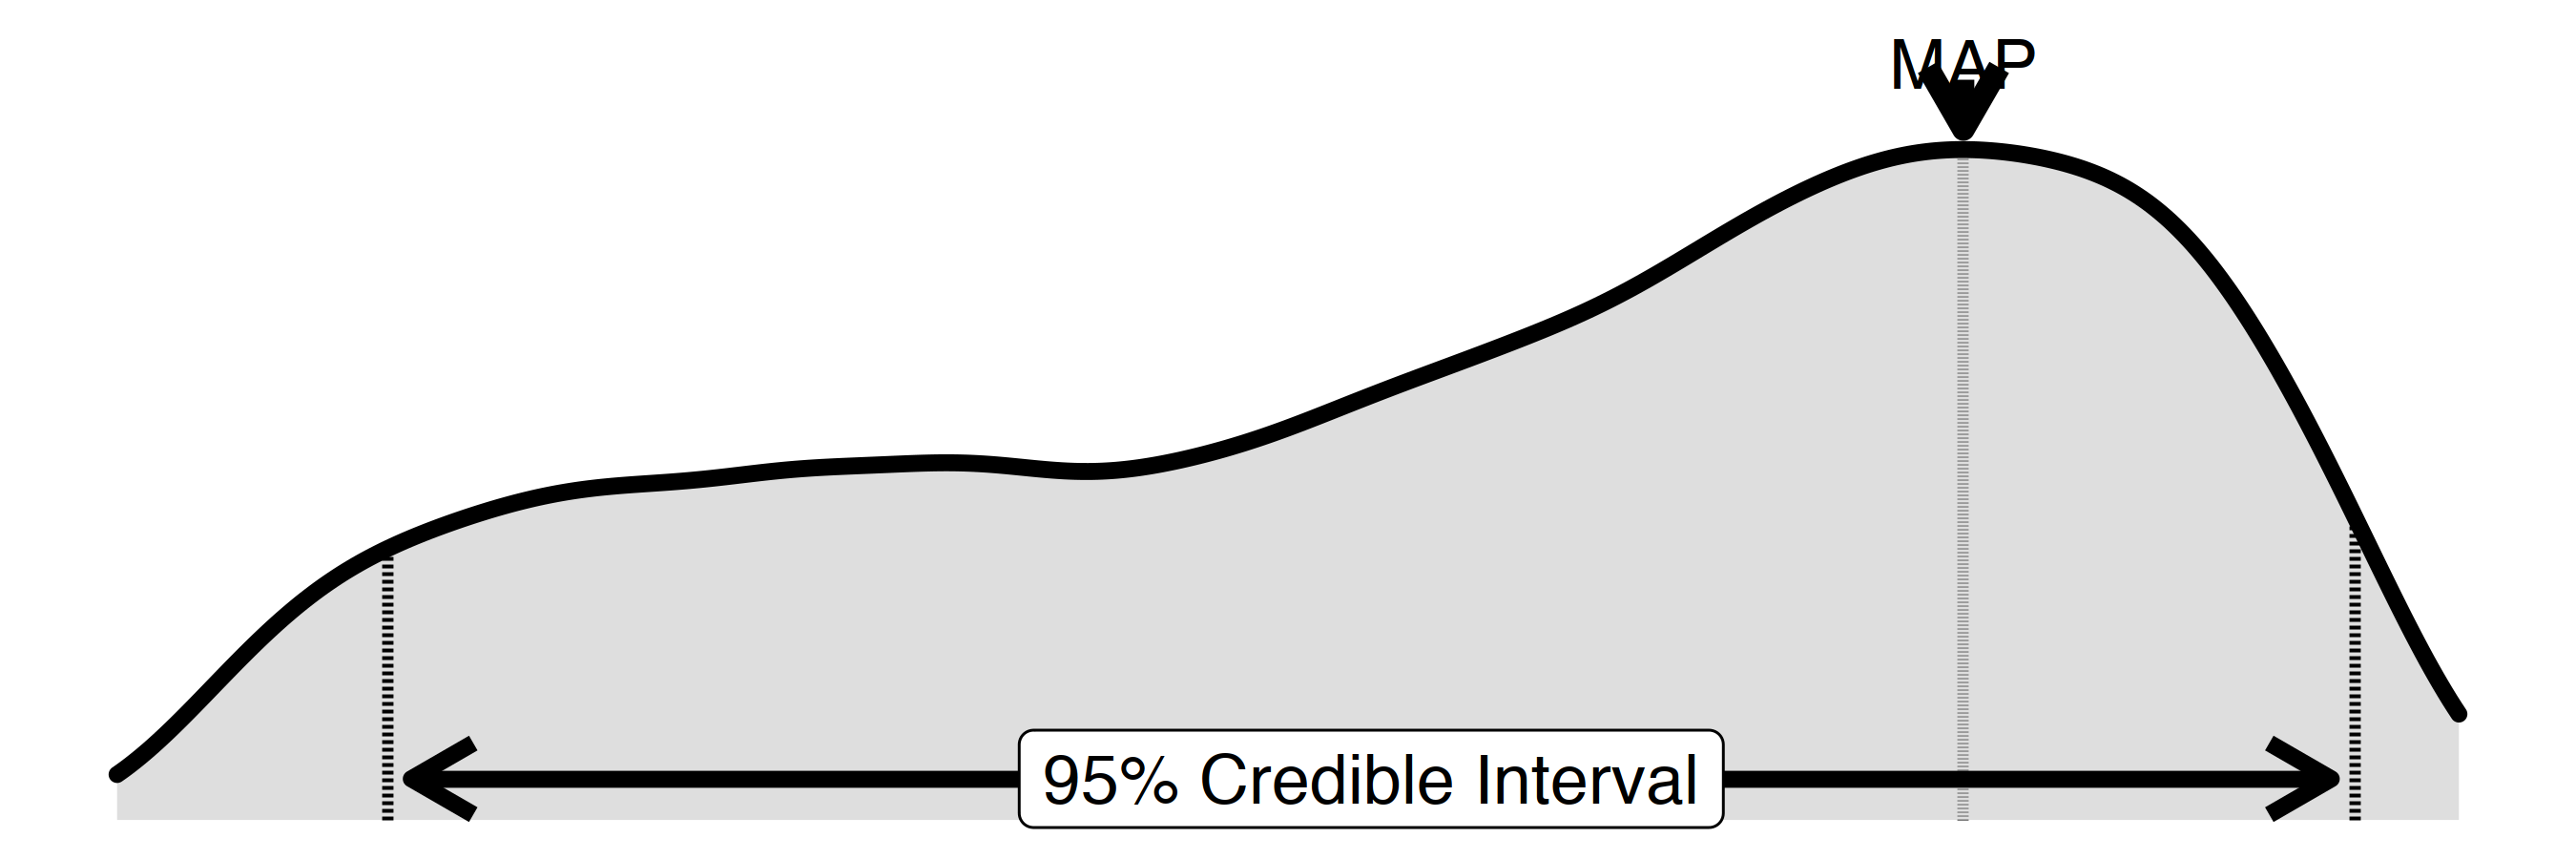
\includegraphics[width=0.8\textwidth]{figures/posterior-1} 

}

\caption{Describing the posterior distribution with an interval, for example the 95\% credibility interval, or a point estimate, for example the maximum a posteriori estimation (MAP).}\label{fig:posterior}
\end{figure}

\hypertarget{from-model-to-world}{%
\section{From Model to World}\label{from-model-to-world}}

Bayesians build \protect\hyperlink{statistical-modeling}{statistical models} to approximate the data-generating process with probability distributions.
These distributions are parameterized, and Bayesians say that these parameters are themselves random variables.
Learning means updating the model parameters.
But after the ``update'' there is no definite answer on what the true parameters are.
Instead, the modeler was able to reduce the uncertainty about the parameters whereabouts.
The posterior distribution doesn't encode the uncertainty inherent in nature, as in quantum mechanics.
Instead, the posterior distribution expresses the uncertainty about \textbf{information about the world}.
That's different from how frequentists connect their statistical models to the world.
Frequentists assume that there are some unknown but fixed parameters that can be approximated with statistical models.
Uncertainty is a function of the estimators, and conclusions about the world are derived from how these estimators are expected to behave when samples and experiments are repeated.

\hypertarget{simulate-to-predict}{%
\section{Simulate to Predict}\label{simulate-to-predict}}

Parameters are random variables.
At first glance, that's a problem if we want to make predictions with the model.
But it's actually a gift and not a problem.
In the Bayesian mindset, predictions are also random variables, not just point estimates.
The distribution of a prediction reflects the uncertainty of the parameters.
Not getting a definite answer or prediction seems inconvenient at first.
But it's much more honest and informative than a point estimate.
The modeler in the Bayesian mindset is encouraged to consider the prediction along with its uncertainty.

To predict, the Bayesian must simulate.
Prediction means marginalizing the distribution of the prediction for a new data point \(X_{new}\) with respect to the distribution of parameters:

\[P(X_{new} | X)_{\Theta} = \int P(X_{new} | X, \theta) \cdot P(\theta | X) d\theta\]

Simulation means that values for the parameters are drawn from the posterior distribution.
For each draw of parameters, the modeler can insert these parameters into the probability distribution of the data and then draw the prediction.
Repeating this process many times yields the posterior predictive density.

\hypertarget{strengths-2}{%
\section{Strengths}\label{strengths-2}}

\begin{itemize}
\tightlist
\item
  Bayesianism allows the use of prior information such as expert knowledge.
\item
  Bayesian inference inherits all advantages of \protect\hyperlink{statistical-modeling}{statistical models}.
\item
  Bayesian inference provides an expressive language to build models that naturally propagate uncertainty. This makes it easy to work with hierarchical data, measurement errors and missing data.
\item
  A general benefit: Bayesian updating is an interesting mental model for how we update our own beliefs about the world.
\item
  Bayesian interpretation of probability is arguably more intuitive than frequentist interpretation: When practitioners misinterpret frequentist confidence intervals, it's often because they interpret them as credible intervals.
\item
  Since Bayesian inference always estimates the full posterior, decision based on the posterior always require another step. As a consequence, inference and decision making are decoupled. In frequentist inference, it's common to design the entire inference process around the decision (hypothesis tests).
\item
  Bayesian statistics adheres to the likelihood principle which states that all the evidence from the data relevant to a quantity of interest must be contained in the likelihood function.
\end{itemize}

\hypertarget{limitations-2}{%
\section{Limitations}\label{limitations-2}}

\begin{itemize}
\tightlist
\item
  The choice of prior distributions is subjective.
\item
  The modeler always has to define a prior which can be tedious when many priors are involved.
\item
  Bayesian methods are mathematically demanding and computationally expensive.
\item
  When used exclusively for decisions, all the additional information about the entire posterior may appear as unnecessary overhead.
\item
  No causal interpretations are allowed, just associations are modeled.
\end{itemize}

\hypertarget{likelihoodism}{%
\chapter{Likelihoodism}\label{likelihoodism}}

\begin{itemize}
\tightlist
\item
  The likelihood function is all you need and is interpreted as evidence for a statistical hypothesis (law of likelihood)
\item
  Statistical hypotheses are compared by the ratio of their likelihoods.
\item
  A \protect\hyperlink{statistical-modeling}{statistical modeling mindset} with \protect\hyperlink{frequent-inference}{frequentism} and \protect\hyperlink{bayesian-inference}{Bayesianism} as alternatives.
\end{itemize}

A frequentist, a Bayesian, and a likelihoodist walk into a bar, a wine bar.
The sommelier quickly joins the three.
The Bayesian wants to hear the sommelier's opinion first before trying the wines..
The frequentist asks the sommelier about the tasting process: is the number of wines fixed in advance? Is the tasting over when the customer has found a suitable wine? How are subsequent wines selected?
The likelihoodist politely tells the sommelier to fuck off.

\protect\hyperlink{frequentist-inference}{Frequentist inference} has a long list of limitations.
But it's still the dominant statistical mindset in science and elsewhere.
Bayesian analysis has seen a resurgence thanks to increased computational power for sampling from posteriors with MCMC.
But using subjective prior probabilities doesn't sit well with many statisticians.
Could there be another way to ``reform'' the frequentist mindset?
A mindset without the flawed hypothesis testing and without priors?

Welcome to the \textbf{likelihoodist mindset.}

I studied statistics for 5 years, worked as a statistician and data scientist for 3 years, and then did PhD studies in machine learning for 4.5 years.
In those 12 years of statistics, I never learned anything about likelihoodism.
It's fair to say that likelihoodism is the underdog.
Likelihoodism leads a shadowy existence while Bayesianism and frequentism are engaged in an epic battle.

Likelihoodism is the purist among the statistical modeling mindsets.
A mindset that focuses entirely on the likelihood function.
Likelihoodism is an attempt to make statistics as objective as possible.

\textbf{All three mindsets use likelihood functions in different ways.}
A quick recap: The likelihood function is the same as the data density function, but the roles of data and parameters are reversed.
Data \(X\) are ``fixed'' and the likelihood is a function of the parameters \(\theta\) \(P(\theta; X) = P(X = x | \theta)\).
The likelihood links observed data to theoretic distributions.
Bayesians multiply prior distributions with the likelihood to get the posterior distributions of the parameters.
Frequentists use the likelihood to estimate parameters and construct ``imagined'' experiments that teach us about long-run frequencies (hypothesis tests and confidence intervals).
Likelihoodists view the likelihood as evidence derived from data for a statistical hypothesis.
Likelihoodists emphasize the likelihood and reject the non-likelihood elements from frequentism and Bayesianism:
Likelihoodists reject priors because they are subjective;
Likelihoodists reject the frequentists' reliance on ``imagined'' experiments because these never-observed experiments violate the likelihood principle.

\begin{figure}

{\centering 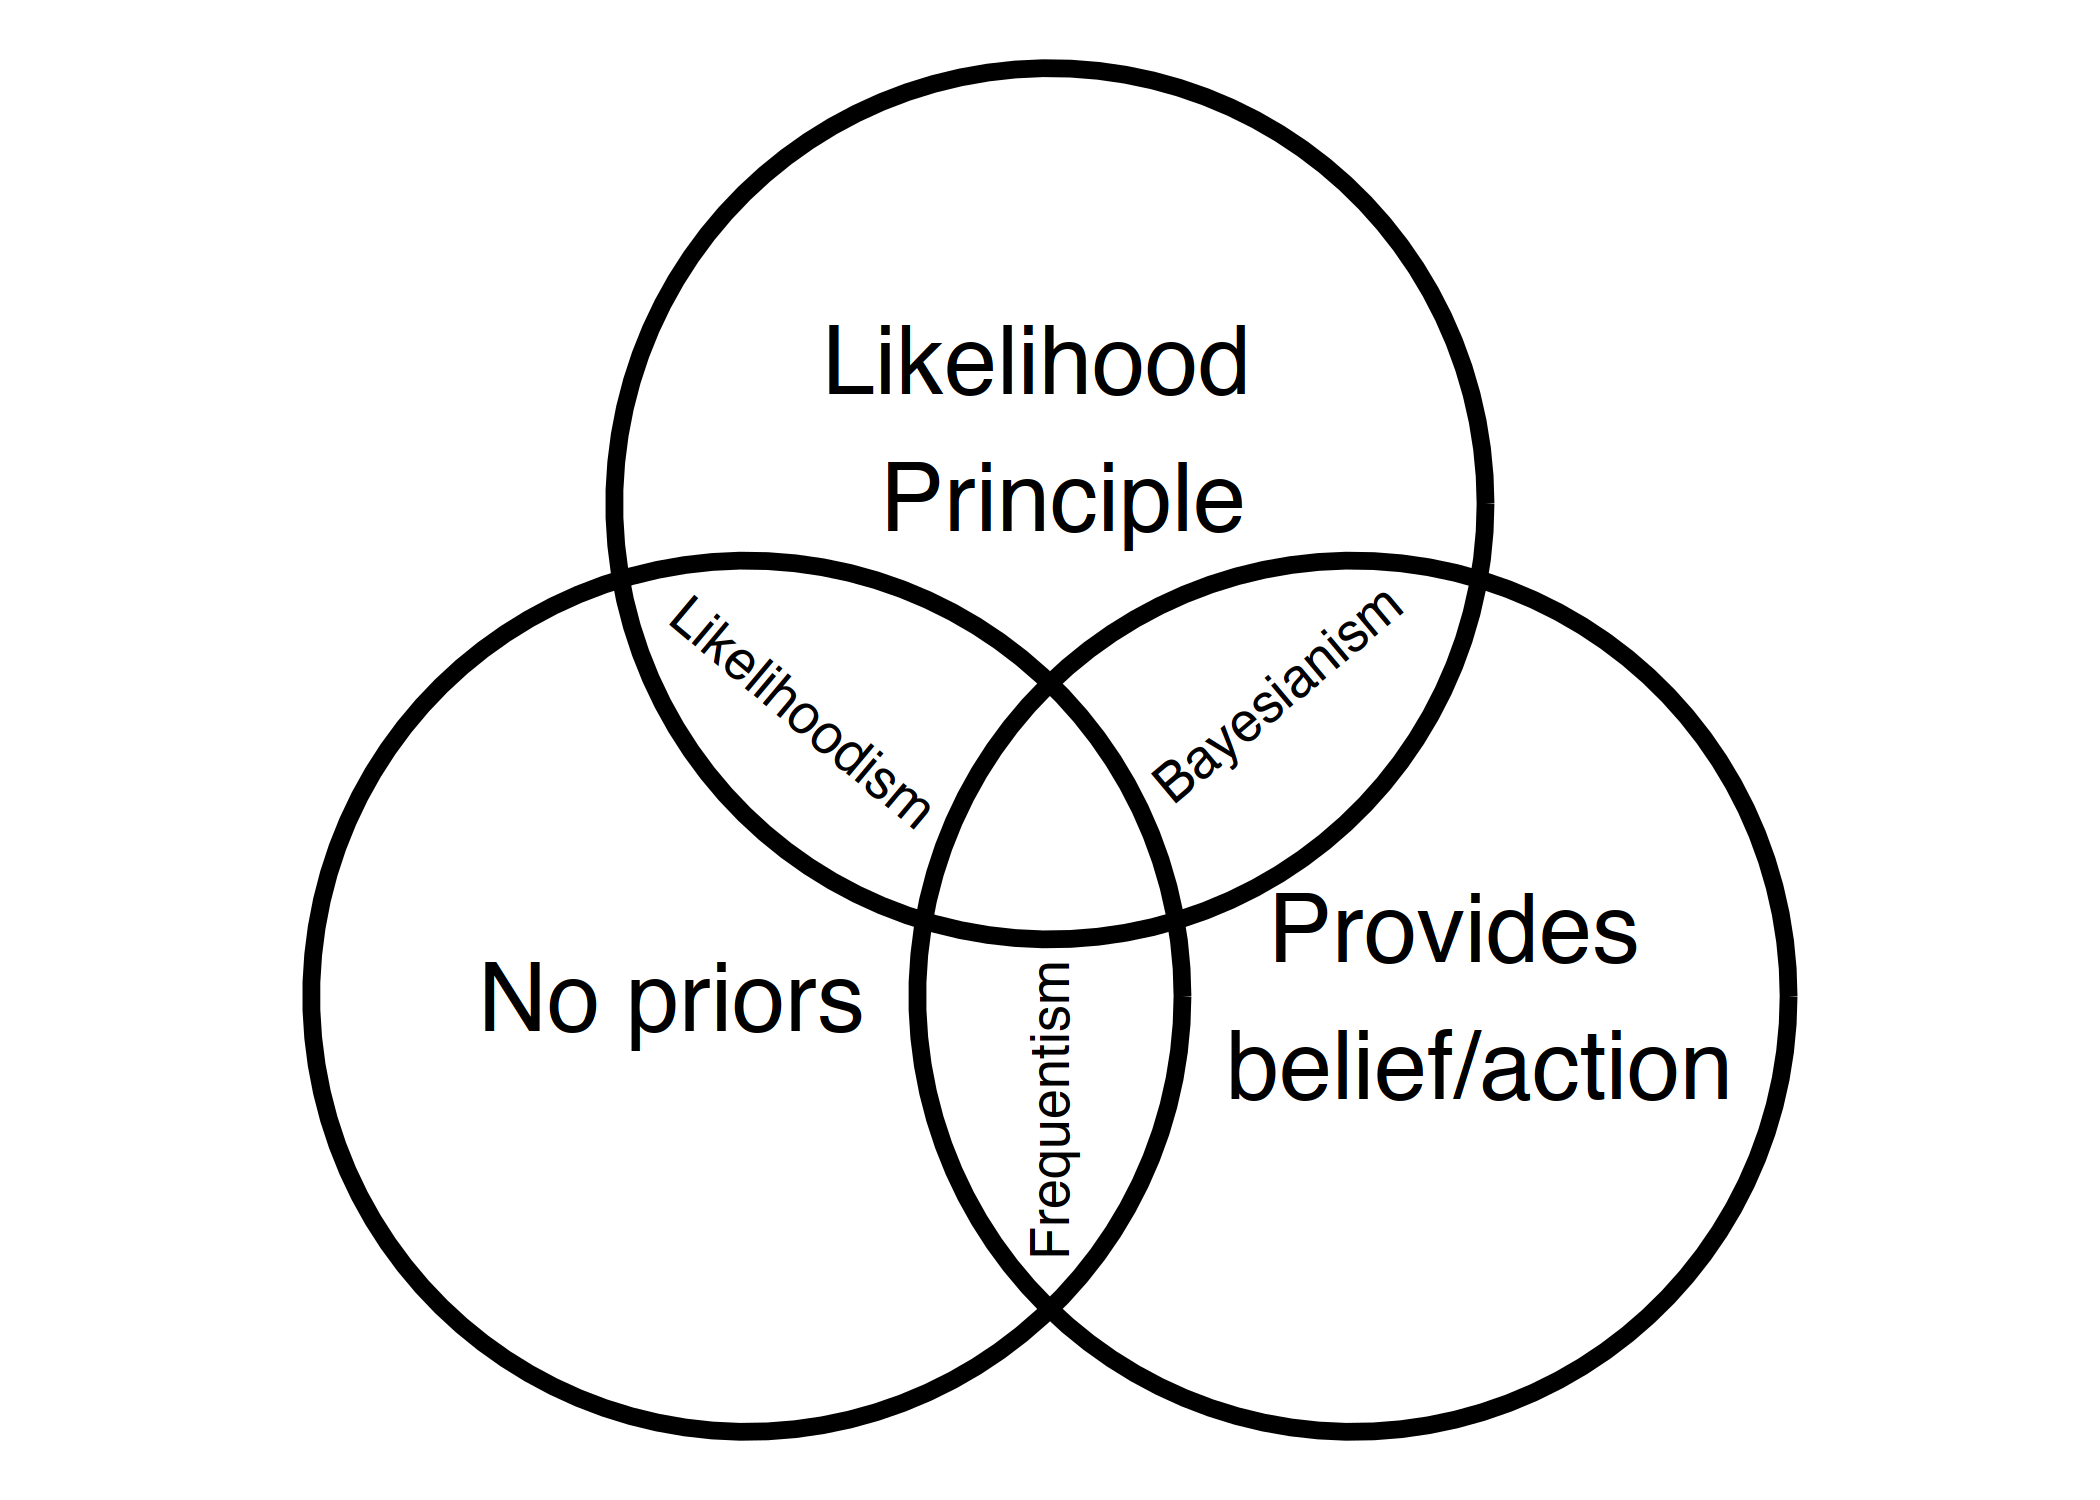
\includegraphics[width=0.8\textwidth]{figures/three-stat-mindsets-1} 

}

\caption{How Bayesianism, frequentism, and likelihoodism overlap and differ. Figure inspired by Greg Gandenberger: https://gandenberger.org/2014/07/28/intro-to-statistical-methods-2/.}\label{fig:three-stat-mindsets}
\end{figure}

But what is the likelihood principle that is so central to likelihoodism?

\hypertarget{likelihood-principle}{%
\section{Likelihood Principle}\label{likelihood-principle}}

``The likelihood principle asserts that two observations that generate identical likelihood functions are equivalent as evidence.''\textsuperscript{\protect\hyperlink{ref-richard2017statistical}{10}}
As a consequence, all evidence that comes from the data about a quantity of interest \(\theta\) has to be part of the likelihood function \(P(\theta;X)\).
If we reverse the statement: If information from the data influences the analysis but is not part of the likelihood, then the likelihood principle is violated.

Let's say we want to estimate the average waiting time for a public bus.
To model waiting times, the exponential distribution is a good choice.
So we could assume that \(X \sim Exp(\lambda)\), where \(\lambda\) can be interpreted as the inverse waiting time.
The expected waiting time is \(\frac{1}{\lambda}\).
We have collected \(n\) waiting times \(x_1, \ldots, x_n\).
The likelihood function is:

\[P(\lambda; x_1, \ldots, x_n) = \lambda^n exp\left(-\lambda \sum_{i=n}^n x^{(i)}\right).\]

In all three mindsets, we could work with this likelihood.
Bayesians would, in addition, assume a prior distribution for \(\lambda\).
Whether the likelihood principle is violated depends on what we do after calculating the likelihood.
Bayesians obtain a posterior distribution for \(\lambda\) that is interpreted as belief about the parameter.
The likelihoodist might report the likelihood region for \(\lambda\), which can be interpreted as relative evidence for a range of parameter values compared to the maximum likelihood estimate for \(\lambda\).
Both the Bayesian and the likelihoodist approaches adhere to the likelihood principle:
All evidence from the data about \(\lambda\) is included in the likelihood.
Bayesians use priors, but as long as they don't include any information from the data, it's fine. \footnote{The likelihood principle is violated when data is used to inform the prior. For example, empirical priors which make use of the data violate the likelihood principle.}

The frequentist might test whether \(\lambda\) is significantly smaller than a certain value.
When performing such a test, the frequentist has to ``imagine'' experiments under the null hypothesis distribution.
But the null hypothesis is not part of the likelihood.
Frequentists choose the distribution under the null hypothesis based on how they ``imagine'' repetitions of the sample or experiment.
This, in turn, depends on how the experiment was conducted or how the data were collected in the first place.
You will see later an example of a coin toss where the same data from different experiments lead to different conclusions in the frequentist mindset.

So the big difference between frequentism and likelihoodism is the likelihood principle.
The likelihood principle gives the likelihood function the monopoly over data evidence.
But the likelihood principle alone is not sufficient to create a coherent modeling mindset.
We need the law of likelihood.

\hypertarget{law-of-likelihood}{%
\section{Law of Likelihood}\label{law-of-likelihood}}

The law of likelihood is the foundation for using the likelihood function alone formaking modeling decisions.
The law of likelihood says\textsuperscript{\protect\hyperlink{ref-hacking1965logic}{11}}:

\begin{itemize}
\tightlist
\item
  Given:

  \begin{itemize}
  \tightlist
  \item
    Hypotheses \(H_1\) and \(H_2\); data \(\mathbf{x} = \{x^{(1)}, \dots, x^{(n)}\}\).
  \item
    Likelihood for \(H_1\) is larger than for \(H_2\): \(P_{H_1}(X = \mathbf{x}) > P_{H_2}(X = \mathbf{x})\).
  \end{itemize}
\item
  Then:

  \begin{itemize}
  \tightlist
  \item
    Observation \(X=\mathbf{x}\) is evidence supporting \(H_1\) over \(H_2\).
  \item
    The likelihood ratio \(P_{H_1}(x)/P_{H_2}(x)\) measures the strength of this evidence.
  \end{itemize}
\end{itemize}

The hypotheses can be the same statistical model, but with different parameter values \(\theta\).
Returning to the bus waiting time example, \(H_1\) could be that \(\lambda = 1\), and \(H_2\) could be that \(\lambda = 0.5\).
The resulting likelihood ratio might be:

\[P(\lambda = 1;x_1, \ldots, x_n)/P(\lambda = 0.5;x_1, \ldots, x_n) = 4\].

The likelihood ratio is the likelihood of one statistical hypothesis divided by the likelihood of another.
As a reminder, statistical hypotheses are statistical models where, optionally, some or all of the parameters are assigned by hand rather than learned from the data.
The law of likelihood tells us, that to compare hypotheses \(H_1\) and \(H_2\) with their likelihood ratio:

\[\frac{P(H_1;X = \mathbf{x})}{P(H_2;X = \mathbf{x})}\]

In frequentism, likelihood ratios are often used as test statistics for hypothesis tests.
In likelihoodism, the likelihood ratio is interpreted as evidence.

Likelihoodists may use a rule of thumb for judging the strength of evidence.
For example, a likelihood ratio of 8 is considered fairly strong and 32 or more is considered ``strong favoring''.\textsuperscript{\protect\hyperlink{ref-richard2017statistical}{10}}
In our example, a likelihood ratio of 4 in favor of \(H_1: \lambda = 1\) over \(H_2: \lambda = 0.5\) is not enough to be ``fairly strong''.
\(H_1\) and \(H_2\) can also be more complex hypotheses, such as regression models with different covariates or assumptions.

\textbf{The law of likelihood is stronger than the likelihood principle:}
The likelihood principle states that the all evidence from the data must be in the likelihood;
\textbf{The law of likelihood describes how evidence can be quantified and compared.}
And this is where Bayesian inference and likelihoodism differ.
Bayesians are not guided by the law of likelihood, but by Bayesian updating and a subjective interpretation of interpretability.

The law of likelihood makes it clear how we can compare statistical hypotheses:
Not by hypothesis testing, but by their likelihood ratios.
The larger the ratio, the stronger the evidence for one hypothesis over another.

This is also where likelihoodism reaches a dead end.
The ratio may only be interpreted as evidential favoring.
The likelihoodist mindset doesn't come with guidance on what we should believe about the parameters or what decision/action to take based on the results.
The likelihood ratio only tell us which hypothesis is favored.

\hypertarget{likelihood-intervals}{%
\section{Likelihood Intervals}\label{likelihood-intervals}}

Likelihood intervals are the likelihoodist analogue to frequentist confidence interval and Bayesian credible intervals.
Likelihood intervals are interpreted in terms of, you guessed it, relative likelihood.
The likelihood interval of a model parameter \(\theta\) is the set of all \(\theta\) values that yield a relative likelihood greater than a certain threshold:

\[\left\{\theta: \frac{L(\theta| X)}{L(\hat{\theta}| X)} \geq \frac{p}{100}\right\}\]

The \(\hat{\theta}\) is the optimal \(\theta\) after fitting the model using maximum likelihood estimation or another optimization method.
Let's say for a logistic regression model coefficient \(\beta_j\): \(\hat{\beta}_j = 1.1\).
Then an interval could be \([0.9; 1.3]\).
The role of the constant \(p\) is similar to the one of the \(\alpha\)-level for confidence and credible intervals:
It specifies the size of the interval.
See figure \ref{fig:likelihood-interval}.
Each \(\theta\)-value within that interval can be seen as constituting a different hypothesis.
And these hypotheses are compared with the optimal model \(\theta = \hat{\theta}\).

\begin{figure}

{\centering 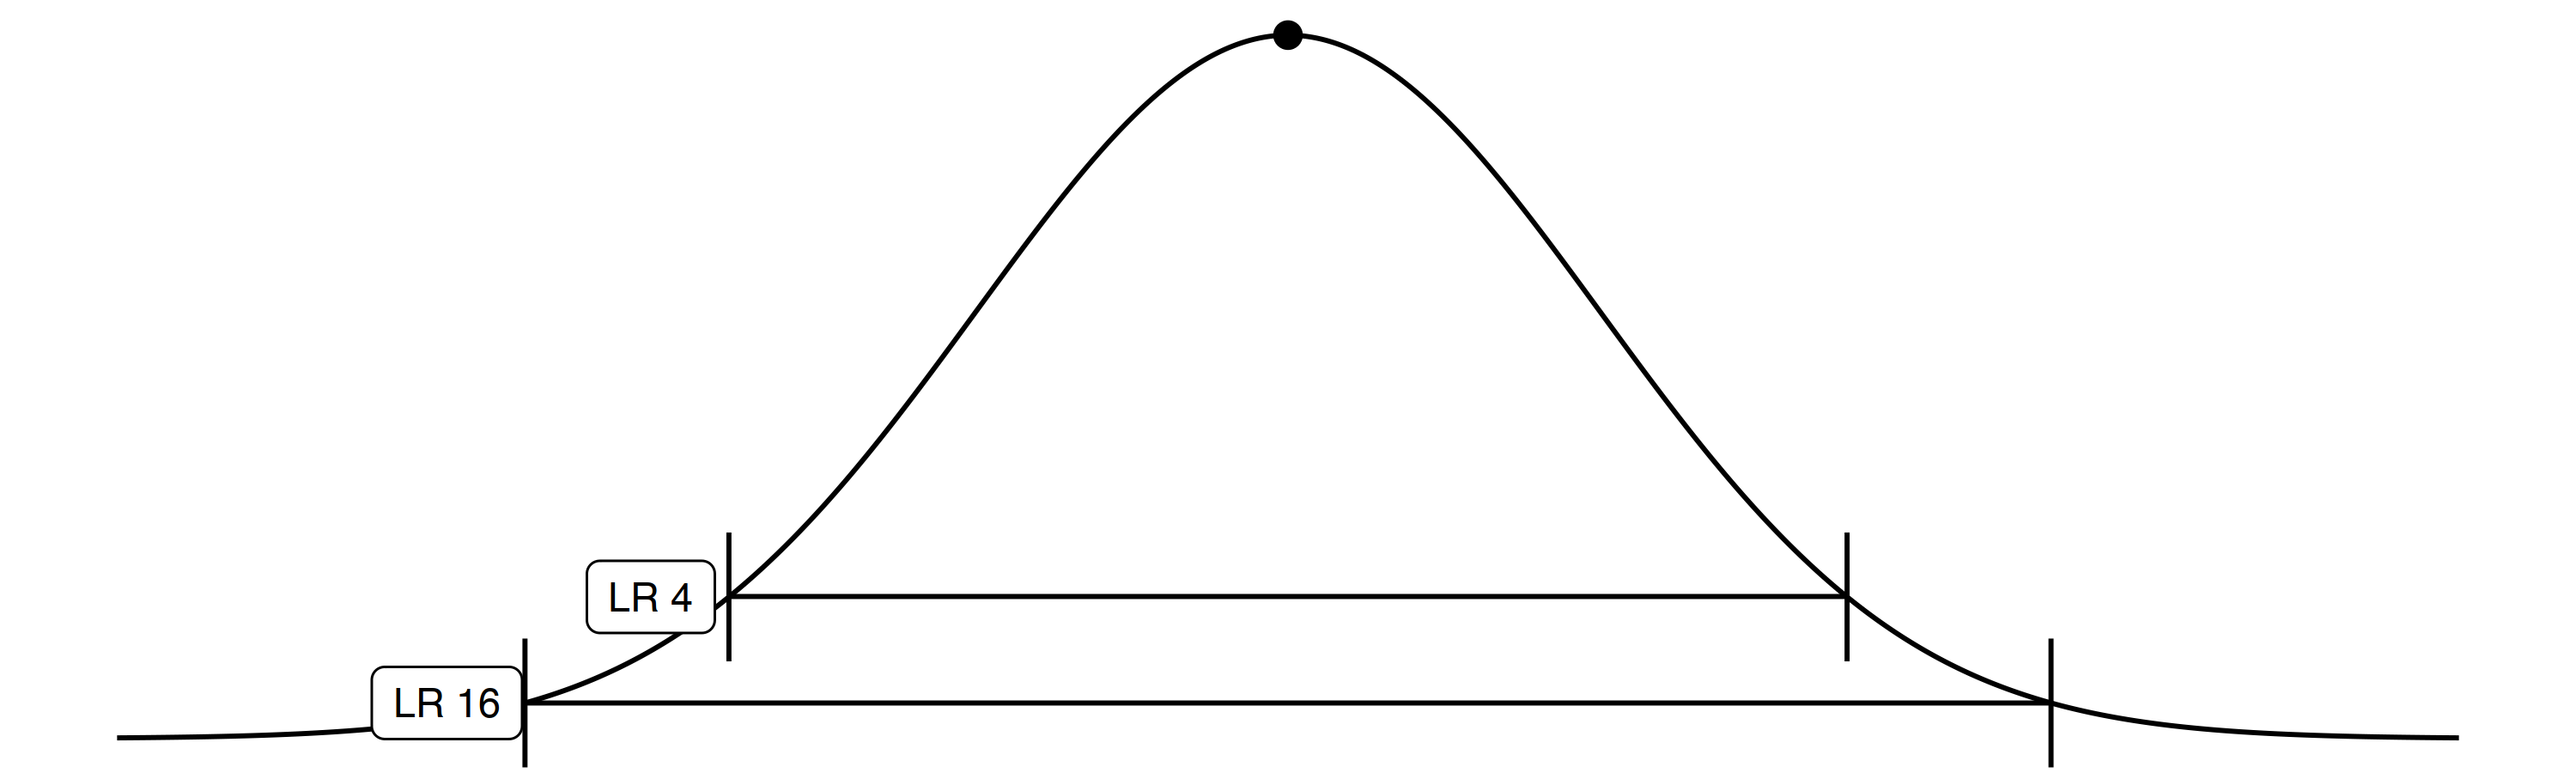
\includegraphics[width=0.8\textwidth]{figures/likelihood-interval-1} 

}

\caption{1/2 and 1/16 likelihood ratio intervals.}\label{fig:likelihood-interval}
\end{figure}

\hypertarget{why-frequentism-violates-the-likelihood-principle}{%
\section{Why Frequentism Violates the Likelihood Principle}\label{why-frequentism-violates-the-likelihood-principle}}

Many frequentist methods violate the likelihood principle because they require ``imagined'' experiments.
But frequentists need these theoretic distribution to compute p-values, for example.
Statistical null hypothesis tests also depend on stopping criteria for data collection, which is in conflict with the likelihood principle.

The following example shows how frequentism violates the likelihood principle because of different stopping criteria.
Suppose we have a coin.
We want to find out whether it's fair, or whether maybe head turns up too often.
I still don't know why statistician's are so upset about unfair coins, but that's the way it is.
We call \(\theta\) the probability of head.
We have two hypotheses:

\[H_0: \theta = 0.5 \text{ and } H_1: \theta > 0.5\]

\(H_0\) means that the coin is fair.
\(H_1\) claims that head comes up more often than tail.
We define two random variables: the number of heads \(X\), and the number of coin tosses \(Y\).

We perform two experiments with a different setup but with the same results:

\begin{enumerate}
\def\labelenumi{\arabic{enumi}.}
\tightlist
\item
  Toss the coin 12 times. We observe head 9 out of 12 times.
\item
  Toss the coin until tail is observed 3 times. The third tail appears on the 12th toss.
\end{enumerate}

Both experiments have the exact same outcome, but we defined the stopping criteria for the experiments differently:
In experiment 1), we fixed the number of tosses \(Y\).
In experiment 2), we fixed the number of heads \(X\).
Should we reach different conclusions about the fairness of the coin?
What do you think?

Both experiments give the same likelihood, up to a constant factor. Experiment 1):

\[L(\theta | X = 3) = \binom{12}{3} \theta^3 (1 - \theta)^9  = 220 \theta^3 (1 - \theta)^9 \]

And experiment 2):

\[L(\theta | Y = 12) = \binom{11}{2} \theta^3 (1 - \theta)^9  = 55 \theta^3 (1 - \theta)^9\]

So the likelihoodists say that both experiments carry the same evidence.
The likelihood intervals would be the same for both experiments.

Frequentists would come to different conclusions depending on the experiment.
Frequentists include results that have not occurred but depend on how the experiments are conducted.
They assume that \(H_0\) is true and infer how the test statistic is distributed in future experiments under \(H_0\).
Then frequentists place the estimated value of \(\hat{\theta}\) within this distribution of imagined experiments and see how extreme the result is.
In experiment 1), where the number of tosses is fixed, experiment outcomes of 9, 10, 11, or 12 heads are more extreme than the actual experiment outcome.
In the other experiment, the number of tails is fixed.
More extreme outcomes in experiment 2) are all possible experiments where we observe more than 12 tosses.
This includes, for example, the experiment where the third tail only comes up after 1108 tosses.

When we test \(H_0\) vs.~\(H_1\) in experiment 1), we get:

\[P_{H_0}(X \geq 9) = \sum_{x = 9}^{12} \binom{x}{12} 0.5^x (1 - 0.5)^{12 - x} = 0.073\]

At a significance level of \(\alpha = 0.05\), we would not reject the fair coin hypothesis.

For experiment 2), we assume a negative binomial distribution:

\[P_{H_0}(Y \geq 12) = \sum_{y=12}^{\infty}\binom{3 + y - 1}{2} 0.5^y 0.5^3 = 0.0327\]

The p-value is now smaller than 0.05, and with that the coin is significantly unfair.

In frequentist inference, the way data are collected and the way experiments are designed affect the results.

This has much more subtle consequences than I've illustrated so far.
Imagine a domain expert asks you to perform an analysis with 1000 data points.
As a frequentist, you need to know how those 1000 data points were collected.
What was the stopping criterion for data collection?
If the domain expert only planned to collect 1000 data points, that's fine.
But if the expert says she would collect more data depending on the outcome of the analysis, then that changes the analysis, which is a violation of the likelihood principle.

\hypertarget{strengths-3}{%
\section{Strengths}\label{strengths-3}}

\begin{itemize}
\tightlist
\item
  Likelihoodism inherits all the strengths of statistical models.
\item
  It's a coherent modeling approach: all information is contained in the likelihood. Frequentism, in contrast, is more fragmented with long lists of differently motivated statistical tests and confidence intervals.
\item
  Like Bayesian inference, likelihoodist inference is also consistent with the likelihood principle. Therefore neither is affected by experimental design, as is the case with frequentism.
\item
  Likelihoodism is arguably the most objective of the statistical modeling mindsets. No priors, no imagined experiments.
\item
  Likelihoodist ideas can improve the reporting of Bayesian results. For example, Bayesians can additionally report likelihood ratios as evidence.
\item
  A significance test might reject \(H_0\), even if the evidence for \(H_0\) is greater than for \(H_1\). Likelihoodism doesn't have this problem.
\end{itemize}

\hypertarget{limitations-3}{%
\section{Limitations}\label{limitations-3}}

\begin{itemize}
\tightlist
\item
  Likelihoodism doesn't provide guidance in the form of belief or decision. Evidence is less practical, and the statistician has no certainty about which the final model is and how to work with it. This is the strongest argument against likelihoodism, and maybe the reason why we don't see it in practice.
\item
  To be more specific: There is no theoretical underpinning for saying when there is enough evidence to choose one hypothesis over another.
\item
  With a likelihoodist mindset, we can can only compare simple hypotheses where all parameters are specified. Composite hypotheses for ranges of parameters are impossible. Likelihoodism can't compare \(\theta > 0\) versus \(\theta \leq 0\). Only, for example \(\theta = 1\) against \(\theta = 0\).
\item
  Likelihoodism allows only relative statements. It can't state the probability that a statistical hypothesis is true -- only how its evidence compares to another hypothesis.
\end{itemize}

\hypertarget{resources}{%
\section{Resources}\label{resources}}

\begin{itemize}
\tightlist
\item
  The book ``Statistical Evidence: A Likelihood Paradigm'' is good introduction to likelihoodism, if you have some background as a statistician.
\item
  I've found the \href{http://gandenberger.org/}{Greg Gandenberger's blog} super helpful in learning about likelihoodism. He takes a more philosophical viewpoint and argues against likelihoodism and for Bayesianism. This critique is most detailed in his essay ``Why I am not a likelihoodist''.\textsuperscript{\protect\hyperlink{ref-gandenberger2016not}{12}}
\end{itemize}

\hypertarget{causal-inference}{%
\chapter{Causal Inference}\label{causal-inference}}

\begin{itemize}
\tightlist
\item
  Causal models place random variables into cause-and-effect relationships.
\item
  A model is a good generalization of the world if it encodes causality.
\item
  Causal inference is not a stand-alone modeling mindset, but causal models are either integrated or translated into a \protect\hyperlink{statistical-modeling}{statistical} or \protect\hyperlink{machine-learning}{machine learning} models.
\end{itemize}

``Thank you for this statistical model,'' the ecologist says to the statistician, and continues, ``Nice p-values and insightful results! Can I conclude from the model that the droughts \textbf{caused} the crop failures?''
The statistician looks at the ecologist, with a hint of concern.
As if practiced, the statistician says, ``Correlation does not imply causation.''
Displeased, the ecologist replies: ``But it would make so much sense to conclude that drought was the cause!''
The statistician looks as if in pain.
``Correlation does not imply causation'', the statistician repeats stubbornly.
``How can we advance science without causality? I want to understand \textbf{why} the crop failures happened,'' the ecologist insists.
``Correlation does not imply causation. Correlation does not imply causation. Correlation \ldots{}'', the statistician now chants, eyes closed, face contorted as if in great pain.
The ecologist slowly backs away, shocked at the statistician's strange reaction.
Sometimes at night, when everything is silent, the ecologist can still hear the haunting calls of the statistician.

\hypertarget{causality-for-the-rescue}{%
\section{Causality for the Rescue}\label{causality-for-the-rescue}}

Some time ago, I worked with a rheumatologist on an important medical question:
Do TNF-alpha blockers reduce long-term symptoms in patients with axial spondyloarthritis, a chronic condition associated with inflammation of the spine.
In the long-term, the spinal joints may fuse due to new bone formation (ossification).
TNF-alpha blockers, given regularly as injections or infusions, work wonders to reduce inflammation.
A clinical trial would have been unethical:
Given the proven effectiveness of TNF-alpha blockers in reducing inflammation, it would have been unethical to give a placebo.
The next best option was to use observational data from hospitals and physician's offices.
The registry of patients with rheumatic diseases for which I worked maintained a huge database of Swiss patients with axial spondyloarthritis.
This database contained valuable data about the patients' health histories:
Physician visits, blood work, x-rays, medication history, and so on.
Working with the rheumatologist, I created a statistical model to see if TNF-alpha blockers could prevent ossification.
For these patients, we had spine x-ray images two years apart, which radiologists used to quantify the progression of bone formation.
To predict progression, the model included several variables measured at the time of the first radiograph: patient age, disease duration, inflammation levels, medication, etc.
The result of the analysis was that the drug didn't reduce ossification.
This finding was somewhat consistent with preliminary research findings of others.

By chance, the lead statistician of the patient registry was taking a course on causal inference at about the same time.
She had the epiphany that our model had a flaw.
She drew a diagram visualizing how the drug, inflammation, and the ossification might be related.
Figure \ref{fig:tnfdag} shows a reduced version of this graph:

\begin{figure}

{\centering 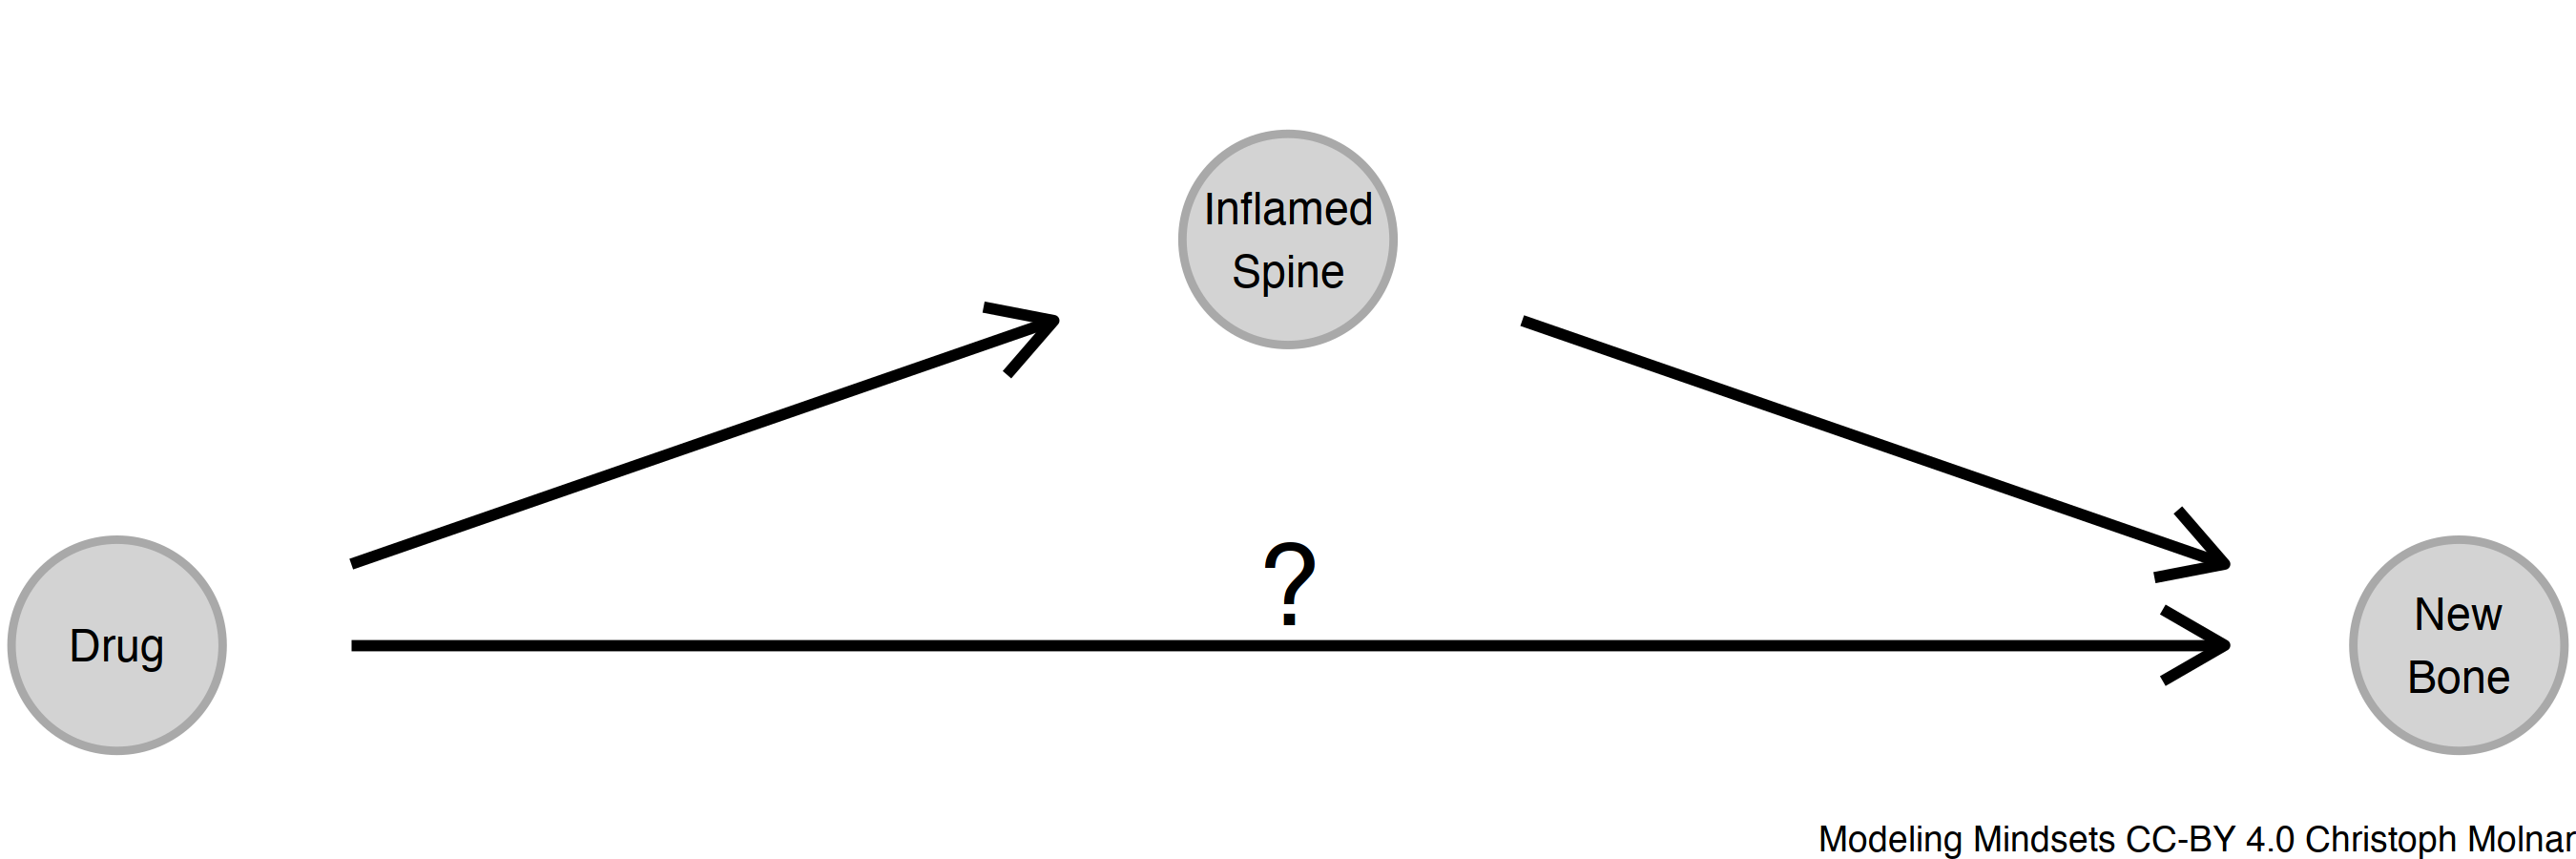
\includegraphics[width=0.8\textwidth]{figures/tnfdag-1} 

}

\caption{The drug was known to influence (reduce) inflammation. Inflammation was thought to cause ossification (new bone formation). The drug can, in theory, reduce ossification in two ways: directly, or indirectly via reducing inflammation.}\label{fig:tnfdag}
\end{figure}

It became immediately clear where the problem lay in our current model:
Inflammation was a potential mediator of the effect of TNF-alpha blockers on long-term ossification.
Figure \ref{fig:tnfdag} shows that the effect of the drug can be divided into a direct and an indirect effect.
The total effect is the direct effect of the drug plus any indirect effects, in this case via reduction of inflammation.
We were interested in the total effect, but the way we built the model, the coefficient for the drug could only be interpreted as a direct effect.
The indirect effect was fully reflected in the coefficient for the inflammation level, which was also included in our model.
We therefore removed the inflammation variable.\footnote{Shouldn't inflammation levels be a confounder because it affects both the decision to treat and the ossification? Or is it a mediator? It depends on the time of the measurement. In the faulty model inflammation was considered after treatment started, making it a mediator of the drug. Later, we adjusted the model to include inflammation before the start of treatment, making it a confounder.}
After removal, the coefficient for TNF-alpha blockers could now be interpreted as the total effect of the drug rather than just the direct effect.
Then the model clearly showed that TNF-alpha blockers reduce ossification by reducing inflammation levels.
This sounds like common sense in hindsight, but coming from a frequentist mindset, I was thunderstruck.
That moment was a real revelation and piqued my interest in causal inference.

\hypertarget{causality}{%
\section{Causality}\label{causality}}

We all have an intuition about causality.
Rain is a possible cause of a wet lawn.
A drug can be a cause of getting well.
An environment policy can be a cause of reduced C02 emissions.
Causality can be expressed as imaginary interventions in random variables:
If you \textbf{force} one random variable to take on a certain value, how would the distribution of another random variable (in the real world) change?
A cause is different than an association:
An association is just a statement about an observation.
We know that a wet lawn does not \emph{cause} your neighbor's lawn to be wet.
How do we know that? Try watering your lawn every day for a year, and see if the probability of your neighbor's lawn being wet has changed.
But the wetness of the two lawns is associated:
If you find that your lawn is wet, the probability that your neighbor's lawn is wet is high.
The reason for this association is, of course, rain.
Such common causes are called confounders.

The archetypal statistician avoids talking about causality.
At least that's my experience, having done a bachelor's and masters in statistics.
What I learned about causality in those 5 years can be summed up two statements: 1) All confounders must be included in the statistical model as dependent variables, and 2) correlation does not imply causation.
We were taught not to interpret statistical models causally and to view causality as an unattainable goal.
We were taught to ignore the elephant in the room.

``Correlation does not imply causation'' is really a mantra you hear over and over again when learning about statistics.
I find this very strange, especially considering that statistical modeling is supposedly THE research tool of our time.
Isn't research all about figuring out how the world works?
The ``how'' implies, at least for me, that scientists are supposed to uncover causal structures.
The truth is that most results are interpreted causally anyways.
By domain experts, by lay people, and by the media.
Whether the statistician likes it or not.
So shouldn't everyone at least try to fit the model with causality in mind?
Fortunately, some people think we should put causality first.

Welcome to the \textbf{causal inference} mindset.

\hypertarget{the-causal-mindset}{%
\section{The Causal Mindset}\label{the-causal-mindset}}

The causal inference mindset places causality at the center of modeling.
The goal of causal inference is to identify and quantify the \textbf{causal} effect of a random variable on the outcome of interest.

Causal inference could be seen as an ``add-on'' to other mindsets such as \protect\hyperlink{frequentism}{frequentist} or \protect\hyperlink{bayesian}{Bayesian} inference, but also for \protect\hyperlink{machine-learning}{machine learning}.
But it would be wrong to see causal inference as just a icing on the cake of the other mindsets.
It's much more than just adding a new type of method to another mindset, like adding support vector machines to supervised learning.
Causal inference challenges the culture of statistical modeling.
It requires the modelers to think more about the data-generating process, to talk explicitly about causes and effects.

It's quite surprising how many models are ``broken'' because they ignore causal reasoning.
A lack of causal reasoning can mean that the analysis of a research paper is invalid, or that a machine learning model in a product is vulnerable to changes in data distribution or adversarial attacks.
Take the Google Flu prediction model as an example.
Google predicted flu outbreaks based on the frequency of Google searches.
The prediction model was clearly not a causal model.
If it were causal, it would mean that you one can could a flu outbreak by searching Google for certain terms.
For example, the flu detection model missed the 2009 non-seasonal flu outbreak.\textsuperscript{\protect\hyperlink{ref-lazer2014parable}{13}}
The machine learning model's performance quickly degraded as search patterns changed over time.
For the causal modeler, a model that relies only on associations is as short-lived as a fruit fly.
A model generalizes well only if it encodes causal relationships.
A causal flu model might rely on the virulence of current flu strains, the number of people vaccinated, forecasts of how cold the winter will be, etc.

You can study the data as closely as you like, but you can't fully discern just from the numbers what causal structures produced those data.
You can automatically infer associations from the data, but even the simplest causal structures are ambiguous.
Sunshine duration on a given day might be considered causal for the number of park visitors.
In a dataset, both variables would appear as columns with numbers in them.
And if we would calculate the correlation, we would find that sunshine and park visitors are positively correlated.
The causal relationship is clear to everyone:
The sunshine duration influences the park visits.
Park visitors don't control the sunshine, and even the smokiest BBQ won't create enough clouds to change the sunshine duration.
But this causal direction is not obvious to your computer.
No matter which of the variables you target, the computer will comply and fit the model.
\emph{Breaking news: The government has banned visits to the park to cool down the current heat wave.}

Assumptions have to be made to decide on causal directions.
These assumptions are often not be testable and therefore a subjective choice of the modeler.
This creates a target for criticism of the causal inference mindset.
On the other hand, causal inference makes causal assumptions explicit and encourages discussions.
When two causal modelers have different opinions a particular causal direction, they have a way of talking about those differences.

Let's take a look at the best way to make causal structures explicit: The directed acyclic graph.

\hypertarget{directed-acyclic-graph-dag}{%
\section{Directed Acyclic Graph (DAG)}\label{directed-acyclic-graph-dag}}

Causal inference comes with a tool for visualizing causal relationships: The directed acyclic graphs, DAG for short.
A DAG, like the one in Figure \ref{fig:dag}, makes it easy to understand which variable is a cause of another variable.
Variables are represented as nodes and the causal direction is illustrated by an arrow.
DAGs must be acyclic, meaning arrows are not allowed to go in a circle.
For example, adding an arrow from \(Y\) to \(X_1\) in Figure \ref{fig:dag} would make the DAG cyclic, and most causal frameworks can't handle that.

\begin{figure}

{\centering 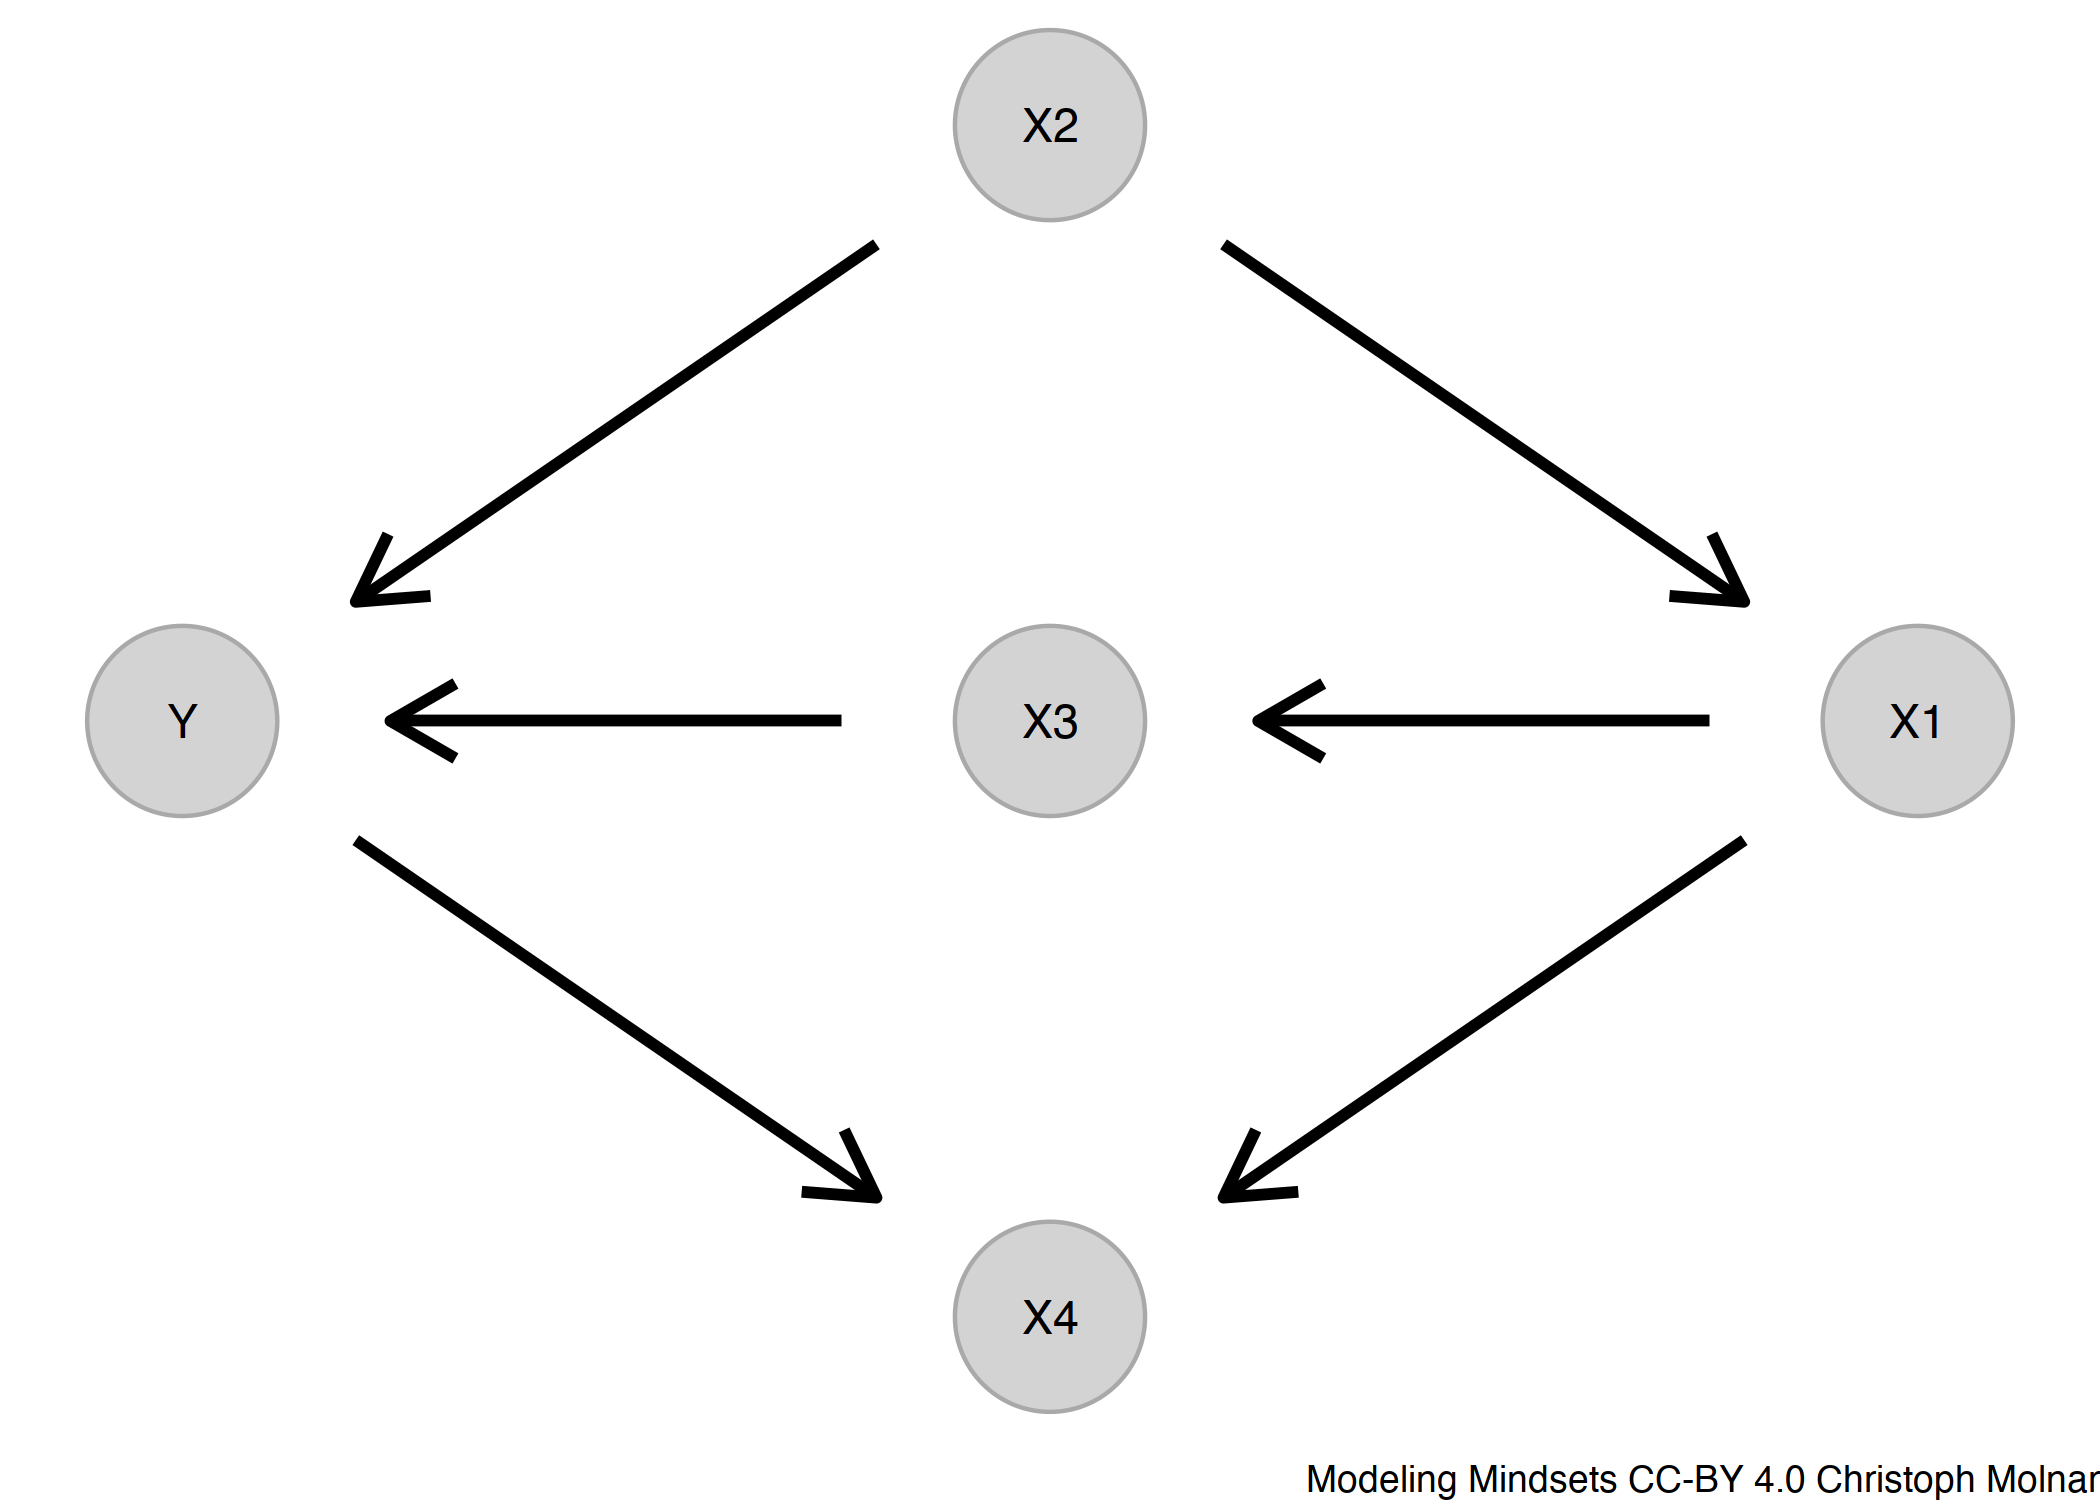
\includegraphics[width=\textwidth]{figures/dag-1} 

}

\caption{A directed acyclic graph (DAG) with 5 variables.}\label{fig:dag}
\end{figure}

What can we see from the DAG in Figure \ref{fig:dag}?
Variables \(X_2\) and \(X_3\) are direct causes of the target \(Y\).
\(X_1\) affects \(Y\) only indirectly through \(X_3\).
And \(X_4\) is not a cause of \(Y\), but \(Y\) causes \(X_4\) together with \(X_1\).

But how do we know where to put arrows and in which direction they should point?
There are several guides here:

\begin{itemize}
\tightlist
\item
  Good old common sense, such as knowing that park visitors can't control the sun.
\item
  Domain expertise.
\item
  Direction of time: We know that the elevator comes because you pressed the button, not the other way around.
\item
  Causal structure learning: To some extent we can learn causal structures automatically. But this usually leads to multiple, ambiguous DAGs.
\end{itemize}

DAG is a great tool for building causal models, but not all approaches rely on DAGs.

\hypertarget{many-frameworks-for-causality}{%
\section{Many Frameworks For Causality}\label{many-frameworks-for-causality}}

There are bewildering number of ``schools'', frameworks, and individual models for causal inference.
And they can differ in notation and approaches.\textsuperscript{\protect\hyperlink{ref-hernan2010causal}{14}}
I find this lack of uniformity is the biggest barrier to entry into the causal inference mindset.
You can choose different introductory books on Bayesian inference, and the basic notation, language and presented methods will be mostly the same.
But causal inference is just a bit more messy.
So don't despair, it's not you, it's causal inference.
Anyway, here is a brief, non-exhaustive overview of causal modeling approaches to give you an idea of what's out there:

\begin{itemize}
\tightlist
\item
  Much causal inference consists of experimental design rather than causal modeling of observational data, such as clinical trials or A/B tests. Causality claims are derived from randomization and intervention.
\item
  Observational data can resemble an experiment, which some call a ``natural experiment''. When John Snow studied cholera, he had access to data from a natural experiment. John Snow identified contaminated drinking water as the source of cholera because customers of one water company were much more likely to get cholera than customers of the other.
\item
  Propensity score matching attempts to estimate the effect of an intervention by matching data points taking into account differences in other variables.
\item
  Probably the most general and coherent framework for causal inference comes from statistician Judea Pearl. This ``school'' includes the do-calculus\textsuperscript{\protect\hyperlink{ref-pearl2012calculus}{15}}, structural causal models, front- and backdoor criteria, and many other tools for causal inference.\textsuperscript{\protect\hyperlink{ref-pearl2009causal}{16}}
\item
  The potential outcomes framework\textsuperscript{\protect\hyperlink{ref-athey2016recursive}{17}} is another larger causal ``school'' used mainly for studying causal effects of binary variables.
\item
  Causal discovery or structure identification is a subfield of causal inference that aims to construct DAGs from observational data.
\item
  Mediation analysis can be used to examine how causal effects are mediated by other variables.
\item
  There are many individual methods that aim to provide causal modeling. One example is ``honest causal forests'', which are based on random forests and used to model heterogeneity in treatment effects.\textsuperscript{\protect\hyperlink{ref-athey2016recursive}{17}}
\item
  \ldots{}
\end{itemize}

All approaches have in common that they start from a causal model.
This causal model can be very explicit, for example in the form of a DAG.
But it can also be hidden in the assumptions of a method.
The final estimate, however, is always a statistical estimator or a machine learning model or something similar.
But how do you get from a causal model to a statistical estimator?

\hypertarget{from-causal-model-to-statistical-estimator}{%
\section{From Causal Model to Statistical Estimator}\label{from-causal-model-to-statistical-estimator}}

In many cases we can't perform experiments because they are infeasible, too expensive or too time-consuming.
But often we have observational data from which we want to infer causal effects.
With observational data, the first casualty is causality -- at least from the point of view of non-causalists.
When causal modelers see observational data, they start stretching and warming up their wrists in anticipation of all the DAG-drawing and modeling to come.

Causal modelers claim that you can estimate causal effects even for observational data.
I am willing to reveal their secret:
Causal modelers use high-energy particle accelerators to create black holes.
Each black hole contains a parallel universe in which they can study a different what-if scenarios.
Joke aside, there is no magic ingredient for estimating causal effects.
Causal modeling is mainly a recipe for translating causal models into statistical estimators, in the following 4 steps:\textsuperscript{\protect\hyperlink{ref-pearl2009causal}{16}}

\begin{enumerate}
\def\labelenumi{\arabic{enumi}.}
\tightlist
\item
  Formulate causal estimand.
\item
  Construct causal model.
\item
  Identify statistical model.
\item
  Estimate effect.
\end{enumerate}

Let's now look at the of the steps.
The first step is to formulate the causal estimand.
That means defining the causes and target that we are interested in.
The estimand can be the effect of a treatment on a disease outcome.
It can be the causal influence of supermarket layout on shopping behavior.
Or it can be the extent to which climate change can be attributed to a particular heat wave.

Once the causal estimand is formulated, we can derive the causal model.
The causal model can be built in the form of DAG.
And while it doesn't have to be a DAG, I think the DAG is the most meaningful ``storage'' and visualization of a causal model.
I addition to the target and potential causes, all other variables relevant to both should be included as nodes in the DAG.
Then the modeler must draw the causal relationships as arrows to finish the DAG.

In the identification step, the causal modeler translates the causal model into a statistical estimator.
Not all causal estimands can be estimated with observational data.
In particular, if a confounder is missing, we can't estimate the causal effect.
Identification can be a complicated, but there are also many simple rules that tell you which variables to include in the statistical model and which to exclude:

\begin{itemize}
\tightlist
\item
  Include all confounders, the common causes of both the variable of interest and the outcome. For example in Figure \ref{fig:dag-rules} \(X_2\) confounds \(X_1\) and \(Y\).
\item
  Exclude colliders. \(X_4\) is a collider for \(Y\) and \(X_1\). Adding colliders to a model opens an unwanted path.
\item
  Exclude mediators. If we want to measure the causal effect of \(X_1\) on \(Y\), we have to exclude \(X_3\). Including \(X_3\) would block the path between \(X_1\) and \(Y\), and we would incorrectly conclude that \(X_1\) has no effect on \(Y\).
\end{itemize}

\begin{figure}

{\centering 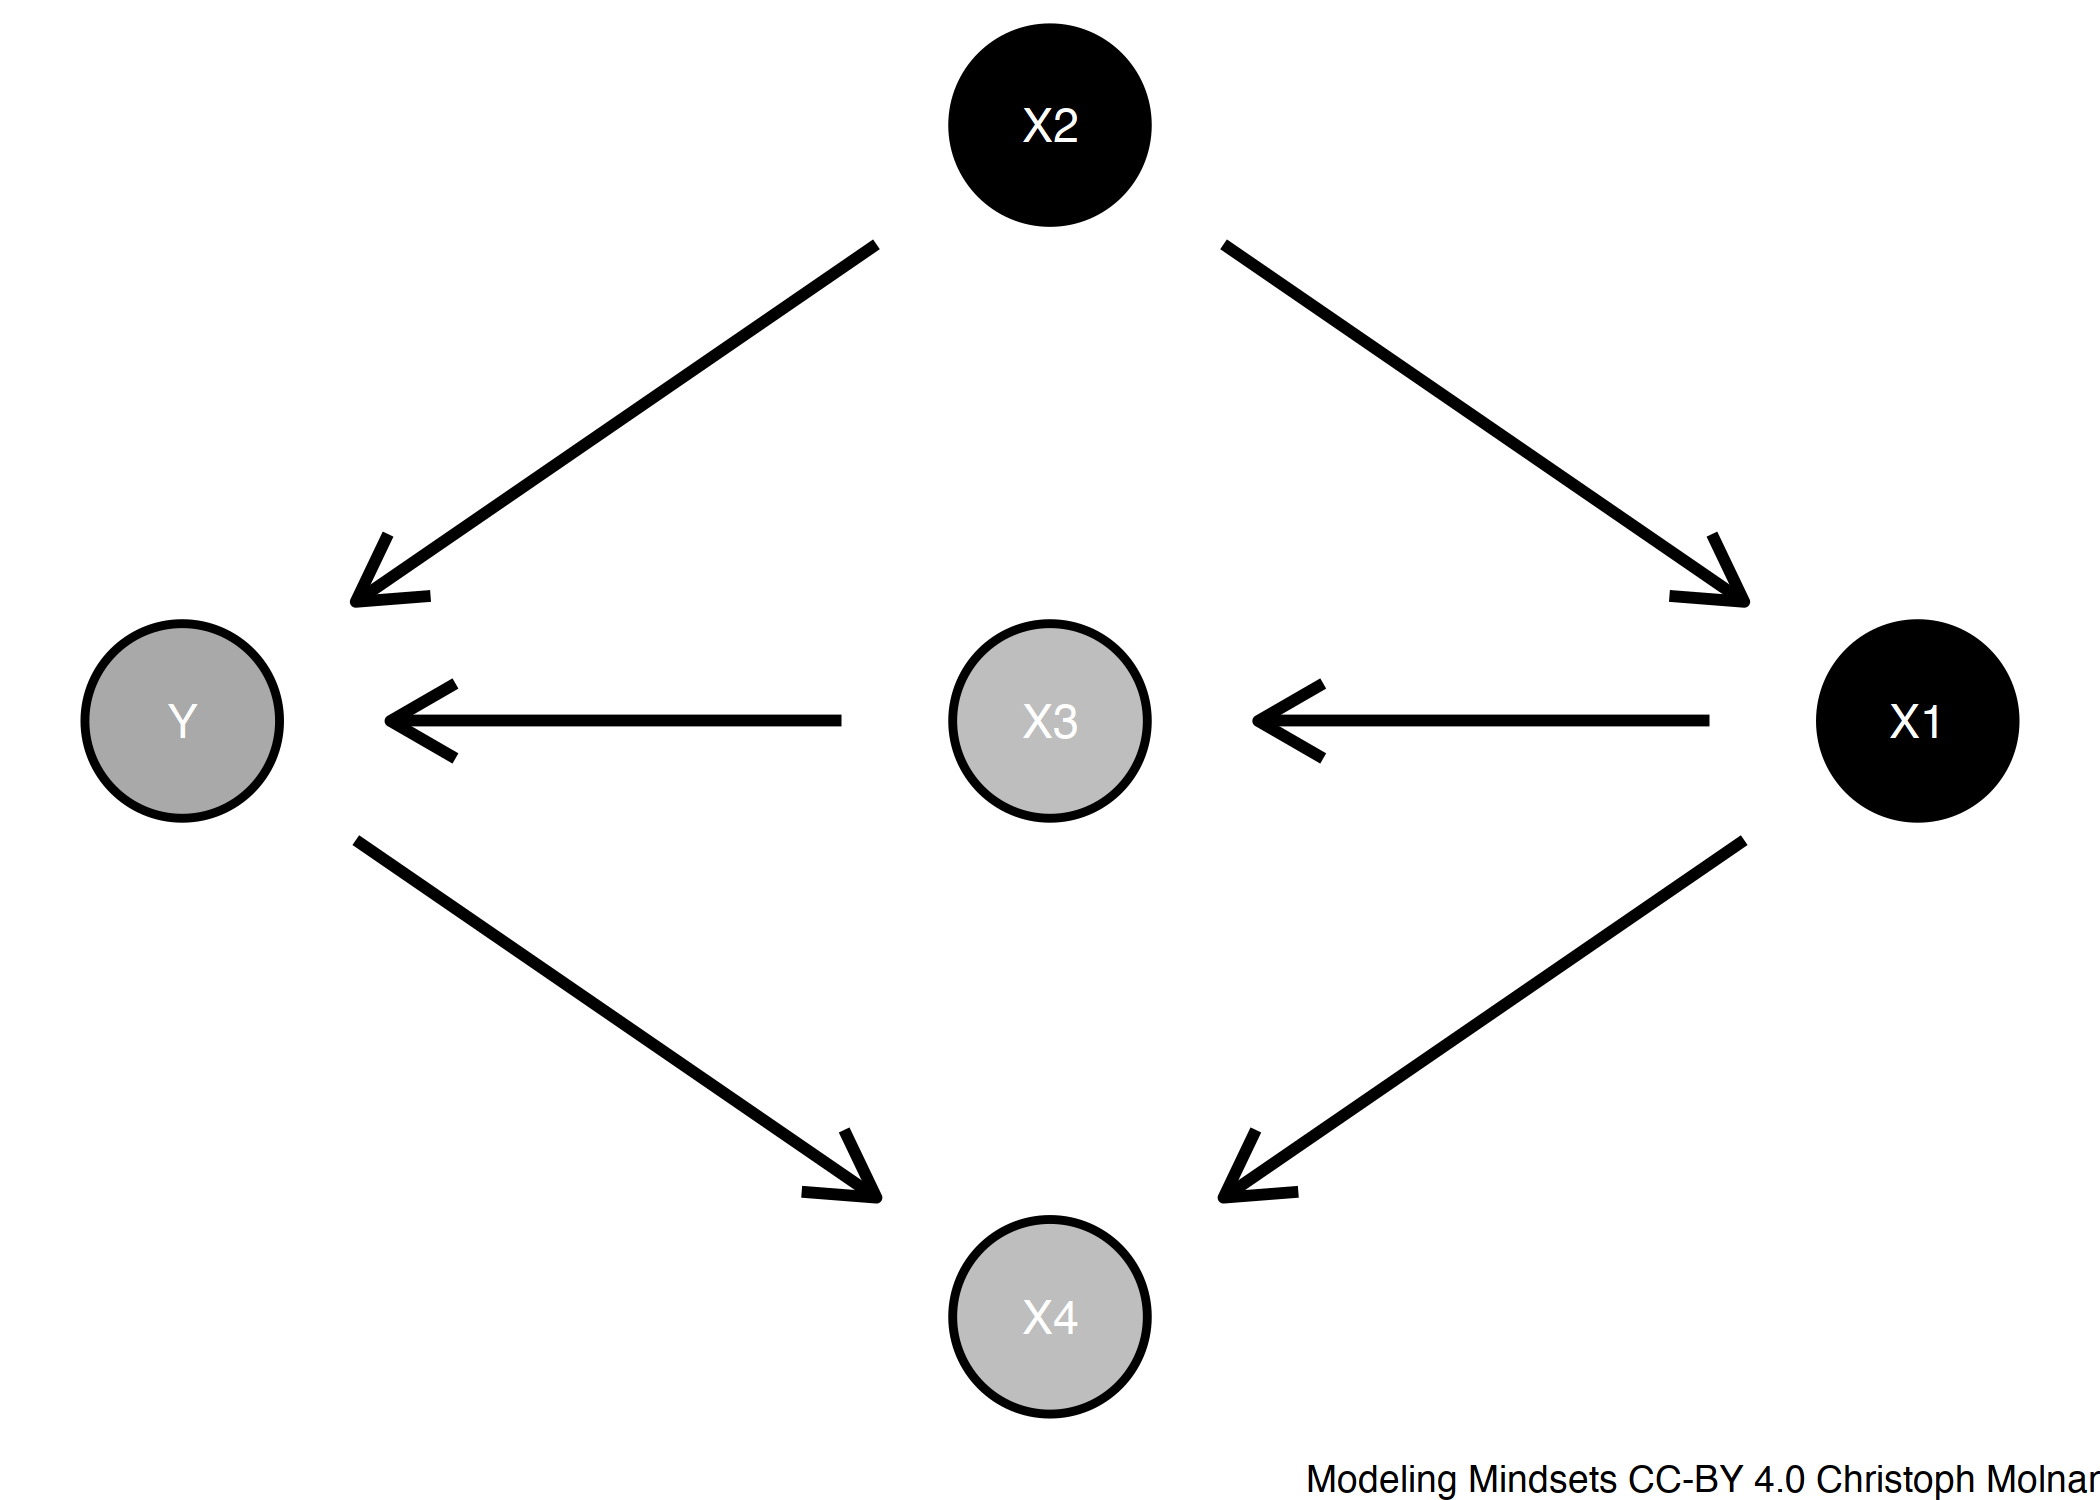
\includegraphics[width=0.8\textwidth]{figures/dag-rules-1} 

}

\caption{To understand the causal effect of $X_1$ on $Y$, we have to build a regression model with $Y$ as the target and $X_1$ and $X_2$ as predictor variables.}\label{fig:dag-rules}
\end{figure}

In the end, we have an estimator or model that can be estimated or fitted without any special magic.
Often it's a regular frequentist or Bayesian model, or a supervised machine learning model.
This means that once the model is estimated, we can interpret the model it as we normally would.
But since the model is also the result of causal reasoning, we may interpret the effect of interest in causal terms.

To estimate causal effects of other variables, all steps must be repeated.
The reason for this is that the identification may lead to a different set of variables for which the model must be adjusted.

\hypertarget{strengths-4}{%
\section{Strengths}\label{strengths-4}}

\begin{itemize}
\tightlist
\item
  Causality is central to modeling the world, and causal inference is \textbf{the} mindset to embrace that fact.
\item
  I think most modelers actually want causal models. Of course, scientists want causal explanations to better understand the world. Modelers in industry also want causal models so they can understand the impact of marketing campaigns, for example.
\item
  Only causal models generalize well because they are more robust to changes in the environment. Or put another way: Non-causal models break down more easily, since they are based on associations.
\item
  Causal inference is a rather flexible mindset that extends many other mindsets such as frequentism, Bayesianism, machine learning.
\item
  DAGs make causal assumptions explicit. If you want to take away just one inside from this chapter, or from causal inference in general, it should be DAGs as a way of thinking and communicating.
\item
  You might say that causal modeling with observational data is not possible. The truth is hat once models are out of the hand of the modeler, in many cases they are interpreted causally. Why then not make an effort to introduce some of the best practices from causal inference?
\end{itemize}

\hypertarget{limitations-4}{%
\section{Limitations}\label{limitations-4}}

\begin{itemize}
\tightlist
\item
  Many modelers stay away from causal inference for observational data because they say causal models are either not possible or too complicated.
\item
  Confounders are especially tricky. For a causal interpretation, you have to assume that you have found all the confounders. But one can never prove that one has identified all confounders.
\item
  There are many schools and approaches to causal inference. This can be very confusing for newcomers.
\item
  Causal modeling requires subjective decisions. The causal modeler can never be sure that the causal model is correct.
\item
  Predictive performance and causality can be in conflict: Using non-causal variables may improve predictive performance, but may undermine the causal interpretation of the model.
\end{itemize}

\hypertarget{further-reading}{%
\section{Further Reading}\label{further-reading}}

\begin{itemize}
\tightlist
\item
  Free book: Causal Inference: What If\textsuperscript{\protect\hyperlink{ref-hernan2010causal}{14}}
\end{itemize}

\hypertarget{machine-learning}{%
\chapter{Machine Learning}\label{machine-learning}}

\begin{itemize}
\tightlist
\item
  Machine learning is a mindset concerned with making a computer ``intelligent''.
\item
  A good machine learning model solves a task well: external evaluation of task performance is more important than the internal validity of the model.
\item
  Machine learning is an alternative meta mindset to \protect\hyperlink{statistical-ml}{statistical modeling}.
\item
  \protect\hyperlink{supervised-ml}{Supervised machine learning}, \protect\hyperlink{unsupervised-ml}{unsupervised machine learning}, \protect\hyperlink{reinforcement-learning}{reinforcement learning}, and \protect\hyperlink{deep-learning}{deep learning} are specializations of the machine learning mindset.
\end{itemize}

It's likely that you've used a machine learning product today.
Maybe you have asked your smart assistant to read out your schedule for today, used a navigation app to get from A to B, or checked your mostly spam-free e-mails.
In all of these applications, machine learning is used to make the product work: speech recognition, traffic jam prediction, and spam classification are just a few examples of what machine learning can do.

\hypertarget{one-or-many-mindsets}{%
\section{One or Many Mindsets?}\label{one-or-many-mindsets}}

Machine learning is the branch of artificial intelligence that deals with learning models directly from data.
The computer improves at a given task through ``experience'' which means learning from data.
The machine learning mindset doesn't tell you \textbf{how} the computer should learn from data.
For example, machine learner may use random variables, but they don't have to.
They can work on a prediction model where it is clearlt of defined when the model is correct, or they can work on clustering where the model is harder to evaluate.
The models can be neural networks, decision trees, density estimators, statistical models and many more.
Given this wide range of tasks, and without strict guidelines on how the computer must learn: Can we really say that machine learning is a distinct mindset?
To answer the question, let's first look at more specific mindsets within machine learning.
Machine learning is usually divided into supervised, unsupervised and reinforcement learning.
Each of these subsets also represents a distinct modeling mindset: They involve a particular view of the world and of the relationship between the models and the world.
The \protect\hyperlink{supervised-ml}{supervised machine learning} mindset frames everything as a prediction or classification problem and has a clear definition of what a good model is: when it generalizes well to new data.
In \protect\hyperlink{unsupervised-ml}{unsupervised machine learning}, the goal is to find patterns in the data.
The \protect\hyperlink{reinforcement-learning}{reinforcement learning} mindset views the world as dynamic, in which an actor interacts with an environment guided by a reward.
In \protect\hyperlink{deep-learning}{deep learning}, all models are neural networks.
What are the commonalities between all these mindsets?
Is there a unified machine learning mindset?

\begin{figure}

{\centering 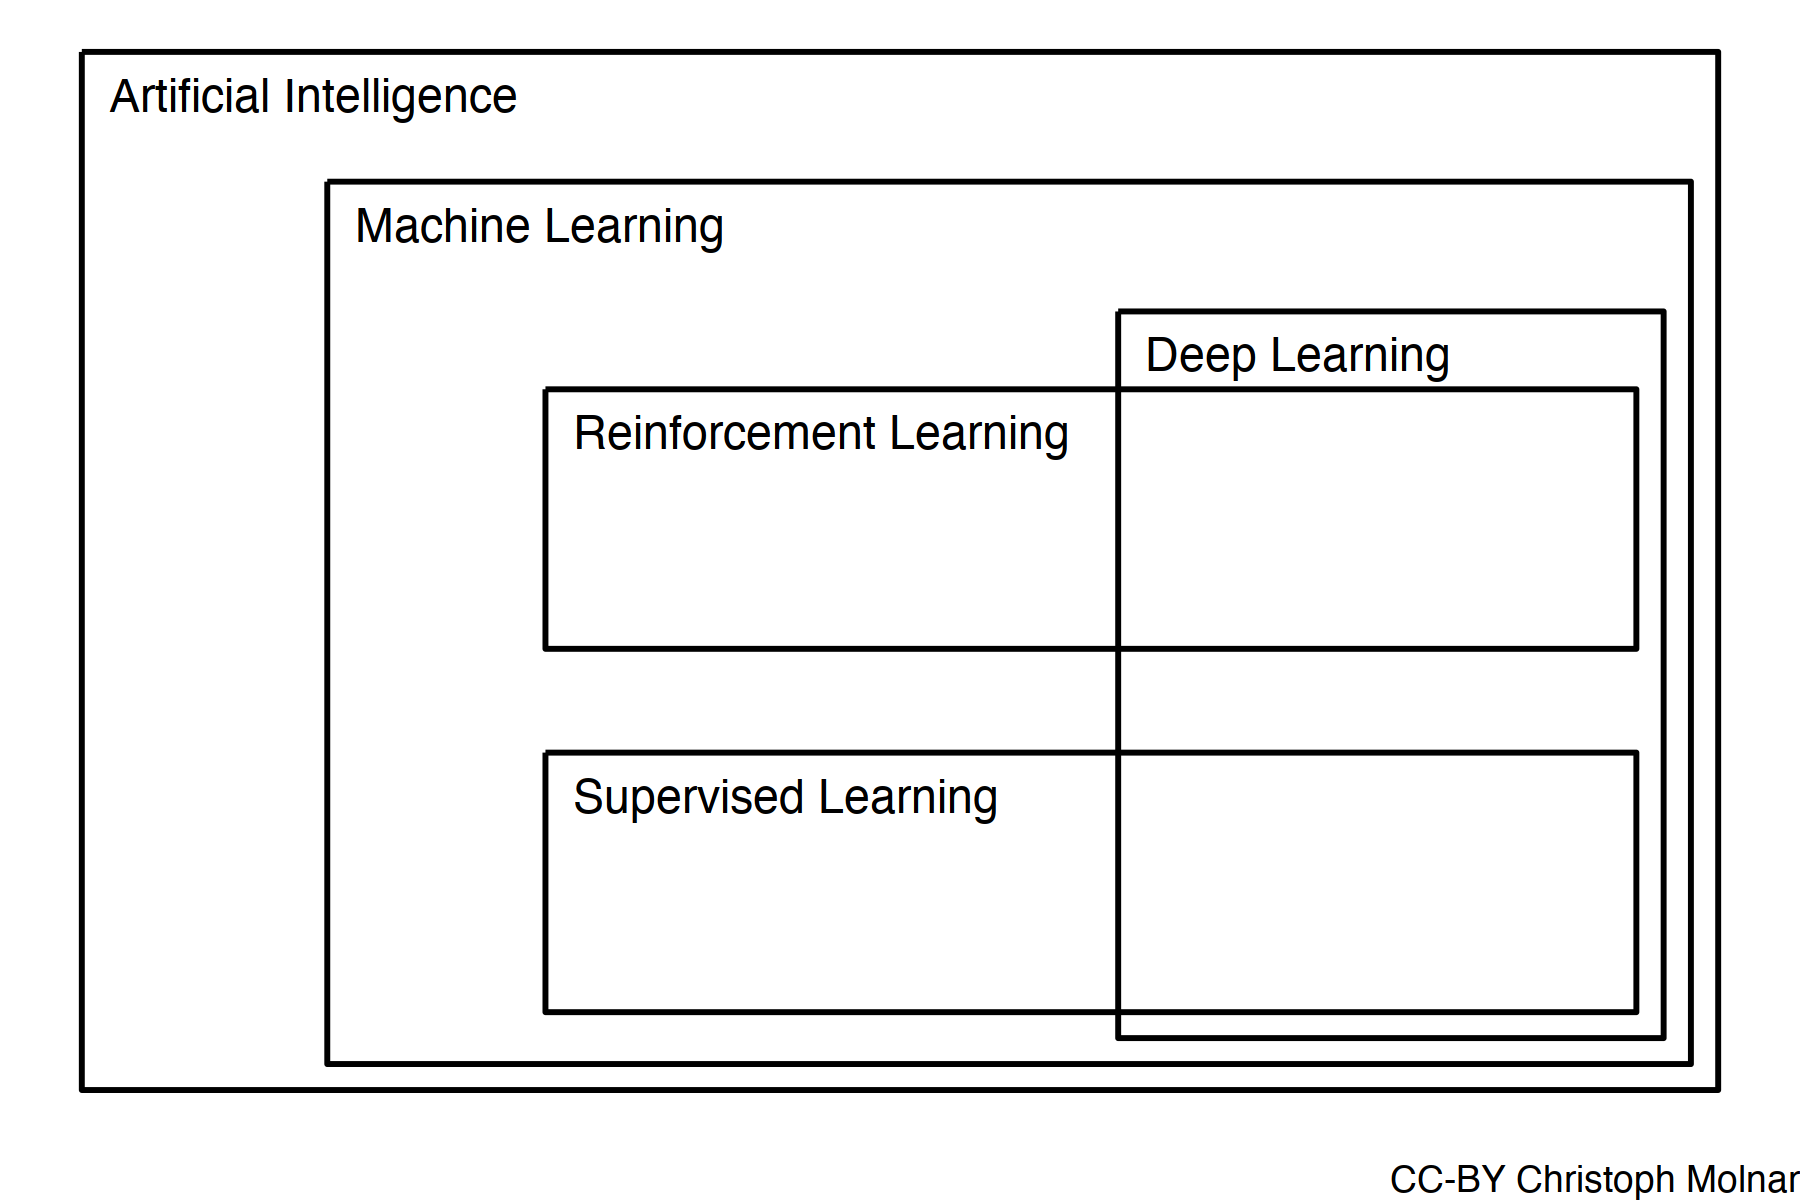
\includegraphics[width=0.8\textwidth]{figures/ml-venn-1} 

}

\caption{Machine Learning is a subfield of artificial intelligence. Within machine learning, there is supervised, unsupervised and reinforcement learning. Deep learning approaches overlap with these three.}\label{fig:ml-venn}
\end{figure}

The machine learning mindset may not be as unified and principled as \protect\hyperlink{statistical-modeling}{statistical modeling}.
But all machine learning approaches have a few things in common.
Let's take a look at what makes a good machine learning model and how these models relate to the real world.

\hypertarget{computer-oriented-task-driven-and-externally-motivated}{%
\section{Computer-Oriented, Task-Driven and Externally Motivated}\label{computer-oriented-task-driven-and-externally-motivated}}

Like all modeling mindsets in this book, machine learning is based on learning models from data.
As the name implies, machine learning focuses on the ``machine'', meaning the computer.
Machine learning is about the computer ``learning'' to solve tasks such as prediction, recommendation, translation, and clustering.
How is this different from the work what statisticians, who also rely on computers?
The motivation for using a computer differs between an archetypal statistician and an archetypal machine learner.
The statistician uses the computer out of convenience and necessity.
Modern statistics wouldn't be possible without the computer.
But the computer is not the starting point.
The starting point is statistical theory.
And the computer is only a tool to apply statistical theory to data. \footnote{There is a field called computational statistics, which is computer-oriented. But we are talking about archetypes of mindsets here. You can think of computational statistics as a statistical mindset that is slightly infused with the machine learning mindset.}
The machine learner, in contrast, starts with the computer.
The machine learner says, ``We have this new thing, the computer. How can we get it do intelligent and useful things?''

Machine learning can be understood as a meta-algorithm:
An algorithm that uses data to produce machine learning models that are also algorithms.
From a programmer's point of view, machine learning is a paradigm shift:
Machine learning is just a way of ``learning'' an algorithm from data, rather than programming it directly. \footnote{I find it difficult to say that the machine learns by itself. Because machine learning also requires programming. You have to implement the learning part and all the glue code to integrate the final model into the product.}

In contrat to more insight-driven statistical mdoeling, machine learning is typically used to solve a task.
The task may be language translation, image captioning, classification, and so on.
The success of the model is measured by how well the task was solved using some type of metric.
In prediction and classification tasks, the machine learner measures the generalization error for new data.
Specifically, for a classification model, this could be the accuracy with which the model assigns classes correctly in a new data set.
In clustering tasks, success metrics usually measure how homogeneous the data points in the clusters are and how much the data differs between clusters.
This external focus is also reflected in the way machine learning research works:
Researchers invent a new machine learning algorithm and show that it works by comparing it to other algorithms in some task benchmarks.
The reason why the algorithm works well is often discovered in later scientific publications, if at all.

We can distinguish between external and intrinsic modeling motivation.
The motivation and evaluation of a machine learning model is external, based on task performance.
It's like judging food based on how it tastes.
Statistical modeling is intrinsically motivated.
The rationale for constructing the model is important.
It's like judging food not only by how it tastes, but also by the cooking process: did the chef use the right ingredients? Was the cooking time appropriate, and so on.

\hypertarget{strengths-5}{%
\section{Strengths}\label{strengths-5}}

\begin{itemize}
\tightlist
\item
  Task-oriented and very practical.
\item
  A job in machine learning potentially pays you lots of money.
\item
  A computer-oriented mindset in a computer-oriented world.
\item
  Machine learning is predestined for automating tasks and building digital products.
\end{itemize}

\hypertarget{limitations-5}{%
\section{Limitations}\label{limitations-5}}

\begin{itemize}
\tightlist
\item
  Not as principled as statistical modeling.
\item
  A confusing amount of approaches with different motivations and technical bases.
\item
  A model that works well in solving a task is not necessarily a good model for insights. A model that predicts diabetes well can be useful, but is less insightful than a statistical model that models diabetes risk explicitly and understandably.
\item
  Often requires a lot of data and is computationally intensive.
\end{itemize}

\hypertarget{supervised-ml}{%
\chapter{Supervised Learning}\label{supervised-ml}}

\begin{itemize}
\tightlist
\item
  Prediction-focused mindset that invites automation and competition.
\item
  A good model has low generalization error - it predicts unseen data well.
\item
  A \protect\hyperlink{machine-learning}{machine learning} mindset.
\end{itemize}

\hypertarget{competing-with-the-wrong-mindset}{%
\section{Competing With the Wrong Mindset}\label{competing-with-the-wrong-mindset}}

It was 2012, and I had just fitted a statistical model to predict whether a patient would develop type 2 diabetes given some risk factors.
And now it was time to test the model.
You see, I wasn't the only one modeling diabetes:
I was competing with many other data scientists.
I uploaded the CSV-file with the prediction results to the competition website.
A table with two columns: One with the patient identifier and one with the probability for that patient to develop diabetes.
One row per patient.
Fingers crossed.
But then came the disappointing results.
The predictions of my model sucked.
What had happened?

At the time, I was a master's student in statistics.
I modeled diabetes risk using a generalized additive model, a model often used in statistical modeling.
Most importantly, I created the model coming from a frequentist modeling mindset.
So I thought a lot about the data-generating process, manually added or removed variables, and evaluated the model based on goodness of fit on the training data.
The statistical modeling mindset failed me in this prediction competition.
And that what confused me at first.
After all, statistical models can be used for prediction and classification, and the same statistical models are also used in machine learning.
Heck! Statistical learning is even one of the foundations of machine learning!
This overlap of theory and methods may mislead one to believe that statistical modeling and supervised machine learning are interchangeable.
But the (archetypal) modeling mindsets are fundamentally different, especially the idea of what makes a good model and how evaluation works.
For me, the disappointing model performance was a catalyst for understanding the supervised machine learning mindset.
For the diabetes competition, I began to seriously study machine learning models like boosting and random forests, but also how to properly evaluate the performance of machine learning models.
While I didn't win any money in the competition (59th place out of 145), I did win something more valuable:
With supervised machine learning, I gained a new modeling mindset.

\hypertarget{predict-everything}{%
\section{Predict Everything}\label{predict-everything}}

In supervised machine learning, everything is a prediction task.
Before complaints come rolling in, here is my definition of prediction:
The proposition of values that are unknown at a given time, but for which a ground truth exists or will exist.
Assigning data points to a cluster is not prediction because there is no ground truth for the clusters.
Prediction can mean assigning a classification score, a numerical value (regression), a survival time, etc.\\
It's amazing how many applications can be formulated as prediction tasks:

\begin{itemize}
\tightlist
\item
  Credit score can be expressed as the probability that someone will repay their loan. Based on information about the person's financial situation, a predictive model assigns a score that indicates how likely it is that the person will pay back the money.
\item
  Predictive maintenance: Many machines require regular inspection and repair. Supervised machine learning models can be used to predict when machines might fail based on current conditions.
\item
  Demand forecasting: using historical sales data to estimate demand for a product.
\item
  Image classification: how should the image be classified? For example, image classification can be used to detect cancer on CT images.
\end{itemize}

As these examples show, supervised machine learning adopts the ``task-oriented'' trait of the machine learning mindset.
Prediction is a task and can be used to do practical things.
A modeling mindset that deals only with prediction tasks seems very narrow.
But there is a surprisingly large number of applications for which prediction can be useful.
And the type of data that can be used in predictive models can also be quite diverse:
The input to the predictive model, usually called features, can be text, an image, a time series, a DNA sequence, a video, a good old Excel spreadsheet, \ldots{}

\hypertarget{supervised-machine-learning}{%
\section{Supervised Machine Learning}\label{supervised-machine-learning}}

Turning any modeling task into a prediction problem is not the only defining trait of the supervised machine learning mindset.
A core idea of supervised machine learning is risk minimization.
And a good supervised model has a low generalization error, meaning that the prediction for new data points is close to the respective ground truth.
To quantify how close a prediction is to the ground truth, the machine learner uses a loss function \(L(y, f(x))\).
The loss function \(L\) takes the ground truth value \(y\) and the predicted value \(\hat{y}\) and returns a number.
The larger the number, the worse the prediction.
In the diabetes example, \(y\) could be 1 for diabetes and 0 for healthy.
Accordingly, \(f(x)\) could be the predicted diabetes probability between 0 and 1.

The goal in supervised machine learning is now to find the function \(f\) that minimizes the loss across the data:

\[\arg \min_{f} L(y, x, f(y))\]

The focus here is on optimizing the loss, and there are no specific constraints on what the function \(f\) may look like.
In statistical modeling, \(f\) would have to be motivated based on probability distributions, but in machine learning, any form is allowed.
This makes supervised learning a true machine learning mindset:
The modeling approach is externally motivated by how the model predictions performs on new data.
The model is trained using one part of the data (training data) and evaluated on another part (test data).

Is there enough to the claim that supervised machine learning is its own mindset?
I believe that supervised machine learning is mindset of its own.
The reason sounds very ``bureaucratic'', but it has strong implications on the mindset: supervised machine learning ALWAYS requires a ground truth.
That's also what separates supervised from unsupervised and reinforcement learning.
We want the model to predict diabetes? For the training data, we actually need to know if a patients have diabetes.
The model is supposed to predict machine failure? We need a data set where we have actually observed many machines, some of which have also failed at some point.

The archetypal supervised learner wouldn't even consider working on unsupervised learning.
For example, I know many machine learning researchers who work exclusively with supervised machine learning.
There is no ground truth, so what the heck should the model ``predict'' anyway?
And even if we defined something that the model should ``predict'', without ground truth we wouldn't really know how to evaluate it properly.
My observation is that in industry people are more pragmatic and it would be harder to find a pure supervised machine learning because there are many problems without labels.

\hypertarget{learning-is-searching}{%
\section{Learning Is Searching}\label{learning-is-searching}}

We have danced around the question of what the function \(f\) is; the function that maps from the features \(x\) to the desired values \(y\).
Without any restrictions on the form of \(f\), finding the best or at least a good \(f\) can seem infeasible.
In statistical modeling it's ``simple'':
We can derive estimators for \(f\) from the theoretical distributions.
This makes the search space much smaller, and searching \(f\) is simplified to finding the best parameterization of a statistical model.
In cases such as the linear regression model, we can even be sure that we have the optimal parameterization.
In supervised machine learning, the loss \(L\) helps us evaluate the \(f\)'s, but it does not tell us how to search for it.

We have to go where the functions \(f\) live:
This would be the hypothesis space.
It's a big space.
I mean, the space has to hold infinitely many functions, even if you have only one feature from which to predict the target \(y\).
In order to search within this space, we have to at least put some constraints on what \(f\) might look like.
And that's where all the different model classes come into play: \textbf{decision trees, support vector machines, linear regression models, random forests, boosting, neural networks}, \ldots{}

For simplicity, let's say we have only one feature \(x_1\) and want to predict \(y\) from it.
The prediction function would then be \(f(x_1)\).
If we restrict \(f\) to be a linear model, we only have to search all \(f\)'s of the form \(f(x_1) = \beta_0 + \beta_1 x_1\).
We have just simplified the search in the vast hypothesis space to the search for the optimal parameters \(\beta_0\) and \(\beta_1\).
A much simpler task.
Similarly, all other machine learning algorithms make the hypothesis space manageable so that it can be searched.
Think of the hypothesis space as a dark forest.
Machine learning algorithms illuminate paths through the forest so that we can search for the best \(f\) within the these paths.
The globally best \(f\) might not be within this illuminated path, so we will usually only find a locally optimal \(f\).
Machine learning algorithms differ in the form and complexity they allow for \(f\).
Decision tree algorithms produce \(f\)'s that look like step functions, since most trees algorithms only allow discrete jumps in prediction.
Neural network are universal function approximators that can, in theory, approximate any function \(f\).\textsuperscript{\protect\hyperlink{ref-hornik1989multilayer}{18}}

Each machine learning algorithm has its own procedure to search the hypothesis space.
Most of the time, this search is about finding the right parameters for a model:
Neural networks use gradient descent with backpropagation to adjust the weights, regression models use maximum likelihood to find the ideal values for the coefficients, and so on.

\hypertarget{overfitting}{%
\section{Overfitting}\label{overfitting}}

Supervised machine learning has one major nemesis: overfitting.
Remember, the goal is to achieve a low generalization error.
But as long as we only use training data, we don't know how well the model will perform with new data.
Worse, machine learning models can easily overfit the training data.
Think of overfitting as memorization of the training data.
When the model perfectly memorizes the training data, it will have have zero loss on the training data, but will likely perform badly with new data.

The opposite of overfitting is underfitting.
If the hypothesis space is too constrained, then model may not be flexible enough to represent the true relationship between the input features and the target.

\begin{figure}

{\centering 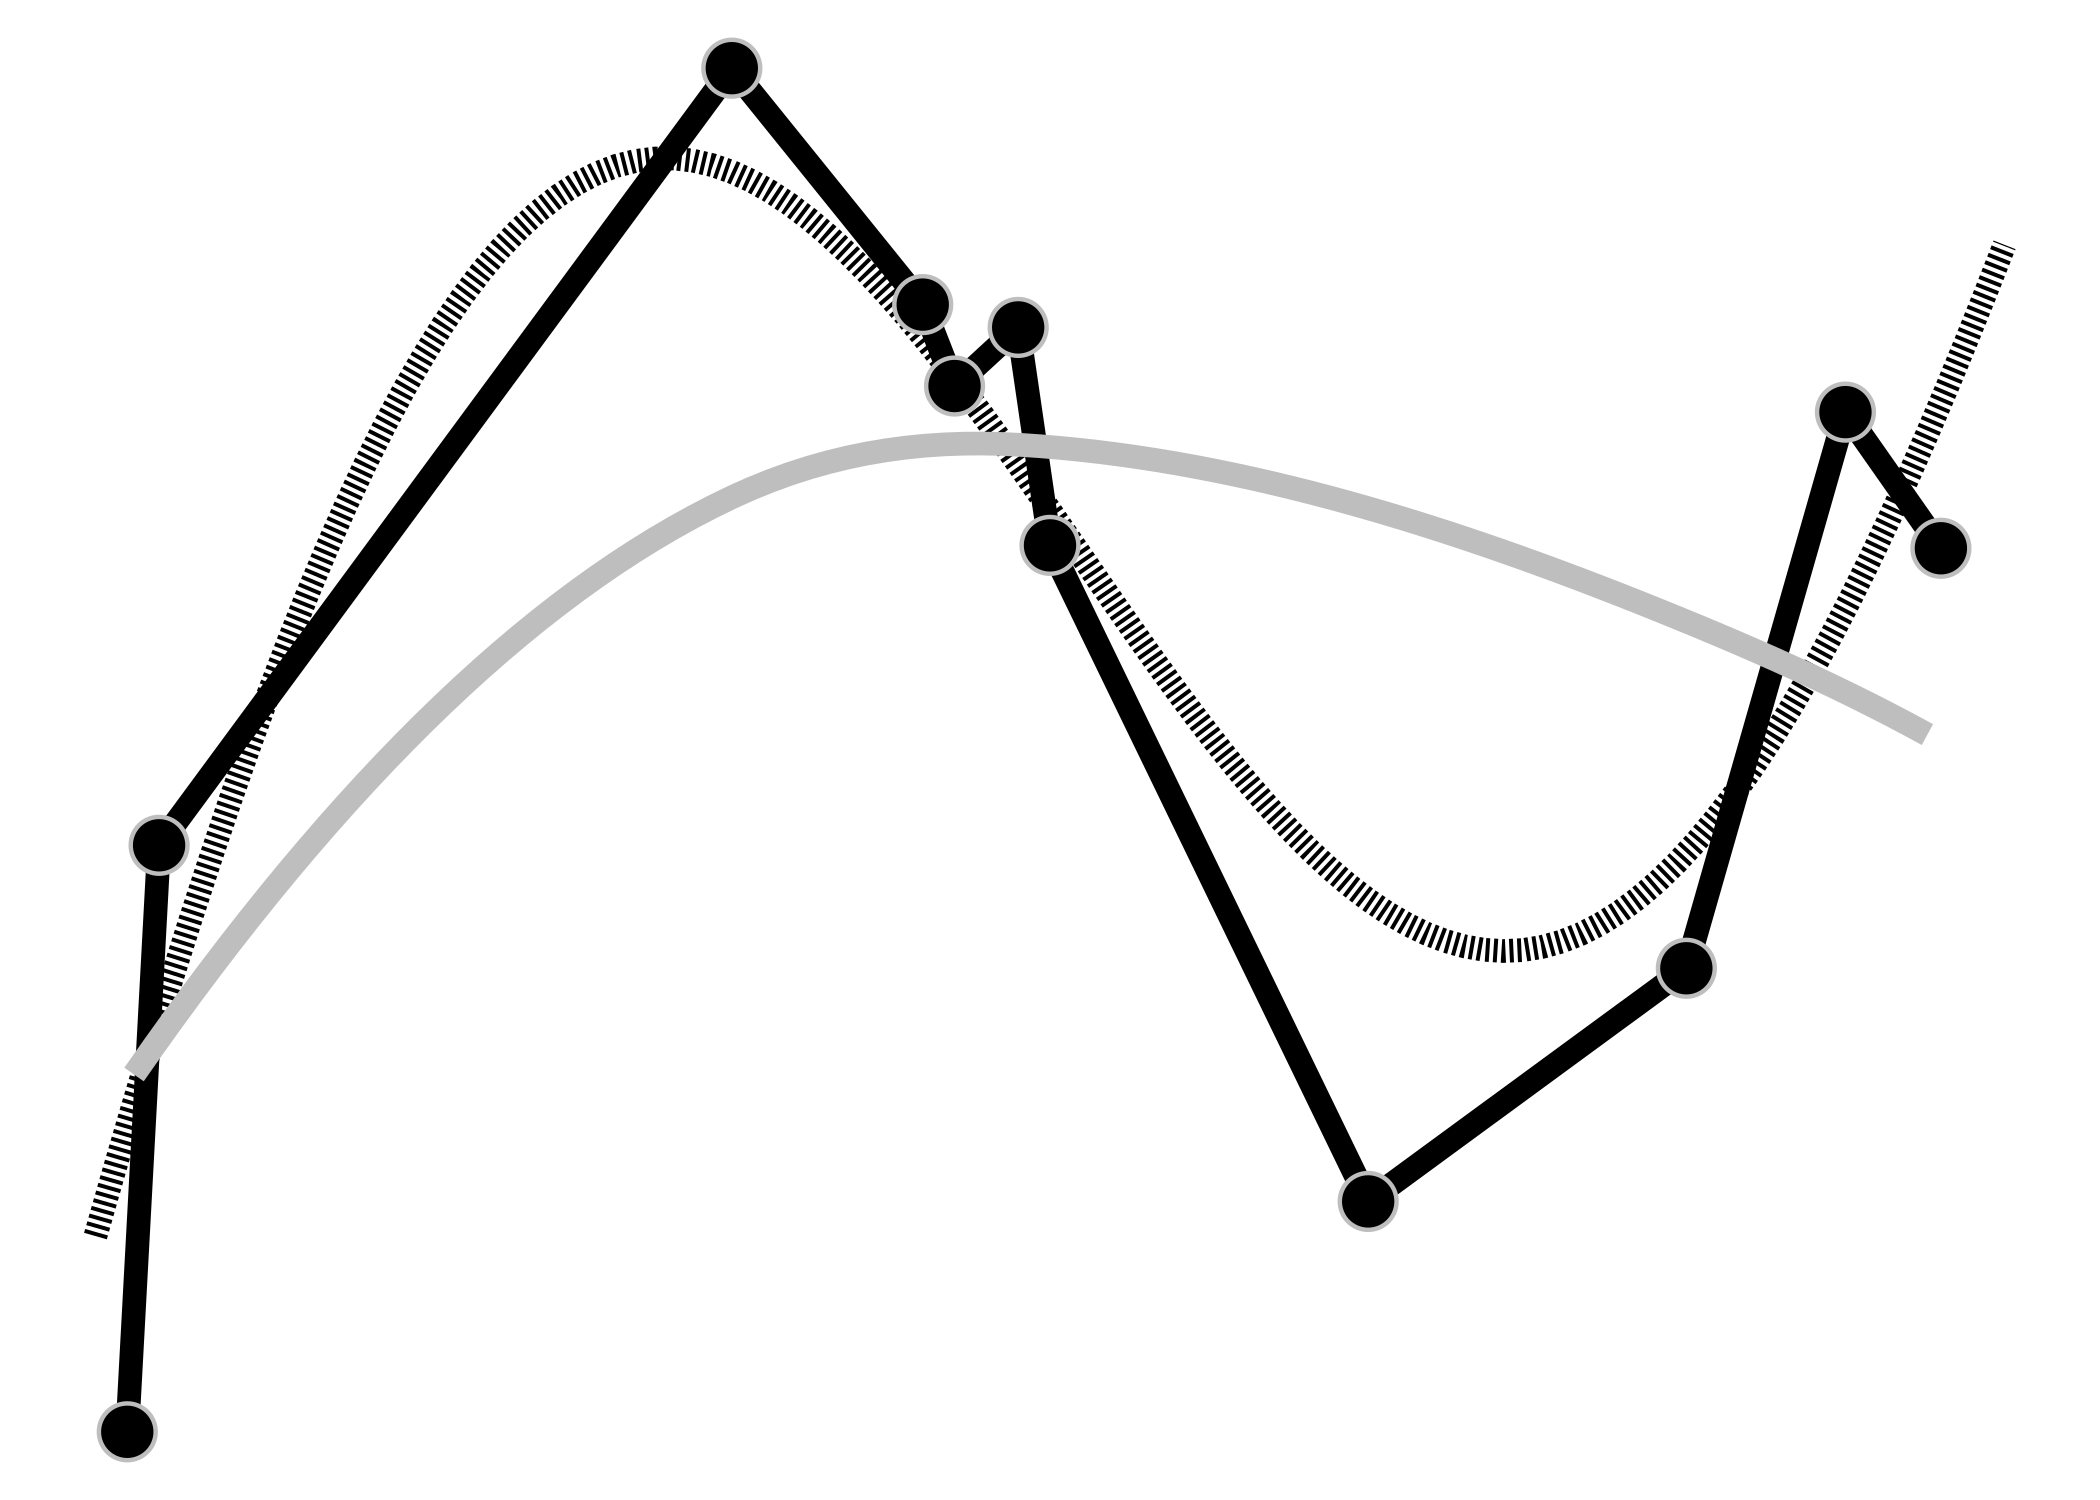
\includegraphics[width=0.8\textwidth]{figures/underoverfitting-1} 

}

\caption{The target y is dependent on x through a function f(x) (dotted line). The observed data (points) have an additional random error. One model overfits the randomness in the training data (black line), and the other underfits (grey line).}\label{fig:underoverfitting}
\end{figure}

Fitting a supervised model means walking a fine line between underfitting and overfitting.
Model evaluation is central to finding this delicate balance and not ending up on one side of the cliff or the other.

\hypertarget{evaluation}{%
\section{Evaluation}\label{evaluation}}

Let's say you want to enter a cooking competition.
A contest with a panel of judges who will evaluate your food and insult you on live TV if it tastes like crap.
You've been practicing your cooking skills for a while.
Fortunately, you have some ``ground truth data'' about how well your food is received.
You cook for family and friends often, and they've given you feedback on how good your dishes tasted.
Over time, your dishes got better and better, and today you consistently get excellent reviews from family and friends.

The jury is the ultimate test of your cooking skills.
You have never cooked for these judges before.
So this test is about how well your cooking skills generalize to new data points.
But are your confident enough about your skills?
What if your supposed kitchen prowess is attuned to strange tastes?
Your your family might be addicted to salt, for example.
And the jurors would be like: ``Did you cook this with seawater?'', ``What is this? Bread? Or a salt lick for goats?''.
In order not to bring shame to your family and name, you decide to validate your skills before this ultimate test.
So you cook for some new people who have never tried your dishes before.
This way you can evaluate your skills without having to waste your shot in the contest.

Rigorous evaluation is close to the heart of supervised machine learners.
A model generalizes well to the real world if the generalization error is low.
A typical recommendation of supervised machine learners is to set up the evaluation pipeline even before training the first model.
In supervised machine learning, evaluation means measuring a loss \(L\) for unseen data, usually called ``test data''.
The test data is like the judges in a cooking competition.
The machine learner may not to use the test data to train the model or test it prematurely.
The test data may only be used for the final evaluation.
If the test data influences the model training or choice in any way, it's ``burned'' and does not show the true performance of the model.
Rather the evaluation will be too optimistic.

Because of this ``burning'' of the test data, machine learners need different strategy to guide their model building.
The test data are set aside.
Whether to compare models or to try different configurations of a model, the machine learner needs unseen data.
The trick is to repeat this train/test split within the training data.
So we cut off a portion of the training data that can be used to evaluate modeling decisions.
This data set is usually referred to as validation data.

\begin{figure}

{\centering 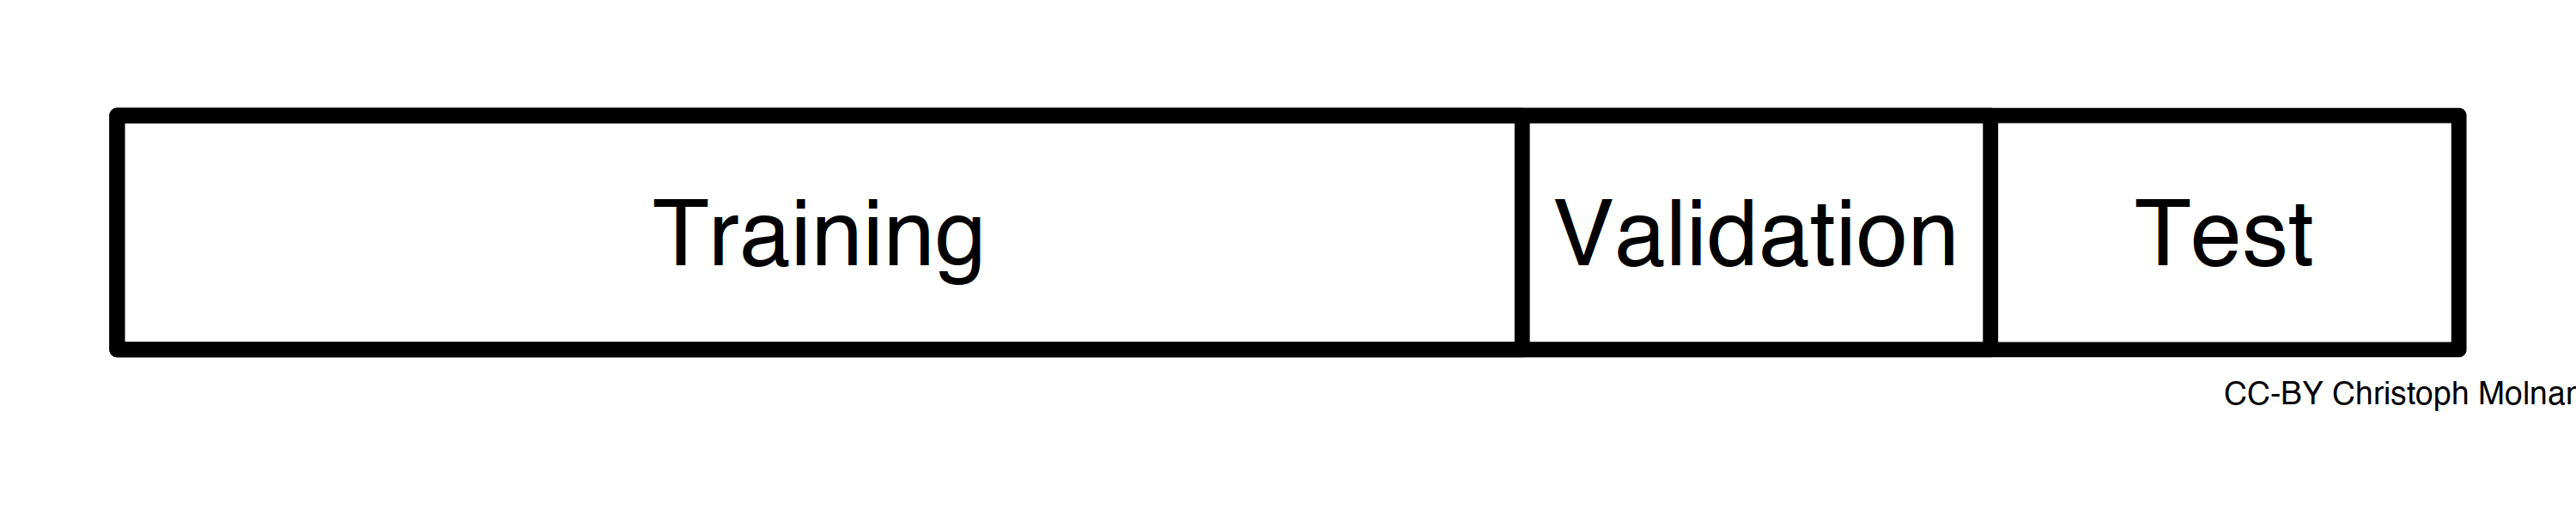
\includegraphics[width=0.8\textwidth]{figures/evaluation-1} 

}

\caption{For evaluation, the data is usually split into training, validation and test data. There are more complex splitting schemes where the data is split multiple times.}\label{fig:evaluation}
\end{figure}

In the simplest version, the data is split once before model training into training, validation and test data.
In reality, techniques such as cross-validation are used to split the data multiple times and reuse the data intelligently.

\hypertarget{an-automatable-mindset}{%
\section{An Automatable Mindset}\label{an-automatable-mindset}}

Supervised machine learning is automatable to a degree that surpasses all other mindsets.
Using a well-defined evaluation procedure, the generalization error, the entire process of model building can be automated.
Supervised machine learning is essentially an optimization algorithm.
In statistical modeling, such as Bayesian and frequentist inference, we have to make all the assumptions, choose the right distributions, decide on the variables to use in the model, look at diagnostic plots, \ldots{}

There is an entire subfield of machine learning, AutoML, that deals with automating the entire training pipeline.
This can include feature engineering, model training, hyperparameter optimization, evaluation, etc.
Automating the supervised machine learning pipeline is computationally intensive, so there is a lot of research on how to automate everything in a smart way.
As a result of this automation capability, there is an entire industry with hundreds of web services and products that automate the training process for you.

But automation is also problematic.
It creates distance between the modelers and the underlying modeling task.
Automation makes modelers less aware of the shortcomings of the data.
On paper, the model may look very good, because the generalization error is small.
But under the surface, the model may be a garbage because it uses features that are not available at the time of the prediction, or the data are terribly biased, or missing data were not handled correctly to, name just a few possible errors.

\hypertarget{a-competitive-mindset}{%
\section{A Competitive Mindset}\label{a-competitive-mindset}}

Another consequence of the one-dimensional evaluation is that supervised learning is a competitive mindset.
Modeling becomes a sport: which is best model for a task?
It also invites competition between people.
Entire websites are dedicated to hosting machine learning competitions where the best modelers can win money.
Sometimes a lot of money.
Your skills as a modeler are reduced to your ability to optimize a single metric.
That metric puts you on the leaderboard, which ranks modelers.
A ranking that ignores many things, such as domain expertise, model interpretability, coding skills, runtime, \ldots{}
The idea of competition has also taken hold of machine learning research itself.
Scientific progress, in large parts, has become a sport.
Progress in machine learning research is when a new machine learning algorithm beats other algorithms in benchmarks.

\hypertarget{nature-statistics-and-supervised-learning}{%
\section{Nature, Statistics and Supervised Learning}\label{nature-statistics-and-supervised-learning}}

As we have seen, the mindsets of statistical modeling and supervised machine learning can be quite different.
At their core, the two mindsets involve different ideas of how to model aspects of the world.
The following comparison is more or less a summary of Leo Breiman's famous article ``Statistical Modeling: The Two Cultures''.\textsuperscript{\protect\hyperlink{ref-breiman2001statistical}{19}}

In the context of prediction, we can think of nature as a mechanism that takes features \(X\) and produces output \(Y\).
This mechanism is unknown and we want to learn about it using models.

\begin{figure}

{\centering 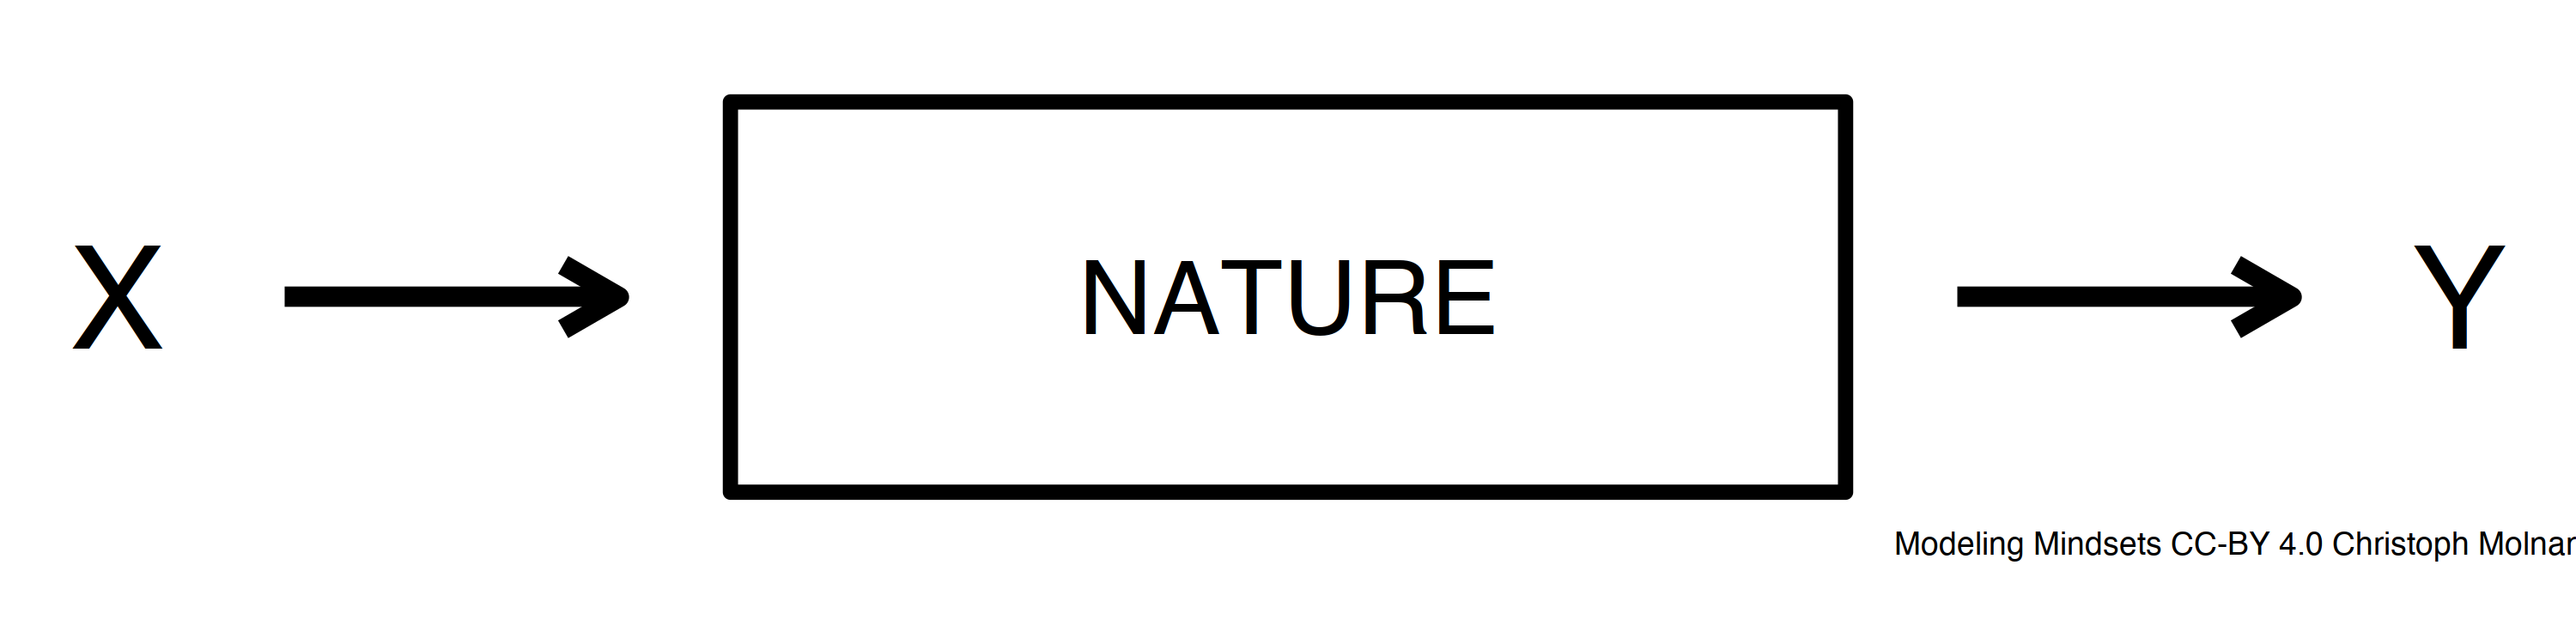
\includegraphics[width=0.8\textwidth]{figures/nature-1} 

}

\caption{Nature}\label{fig:nature}
\end{figure}

Statistical modelers fill this box with a statistical model.
The statistical model is supposed to represent nature.
It is supposed to reproduce the inner workings of nature.
If we are somewhat convinced that we have found the mechanism, we can then take the model parameters and interpret them as if it was the true mechanism in nature.
Nature's true mechanism is unknown and not fully specified by the data, we have to make some assumptions about the forms of this mechanism, which we represent with the function \(f\).

\begin{figure}

{\centering 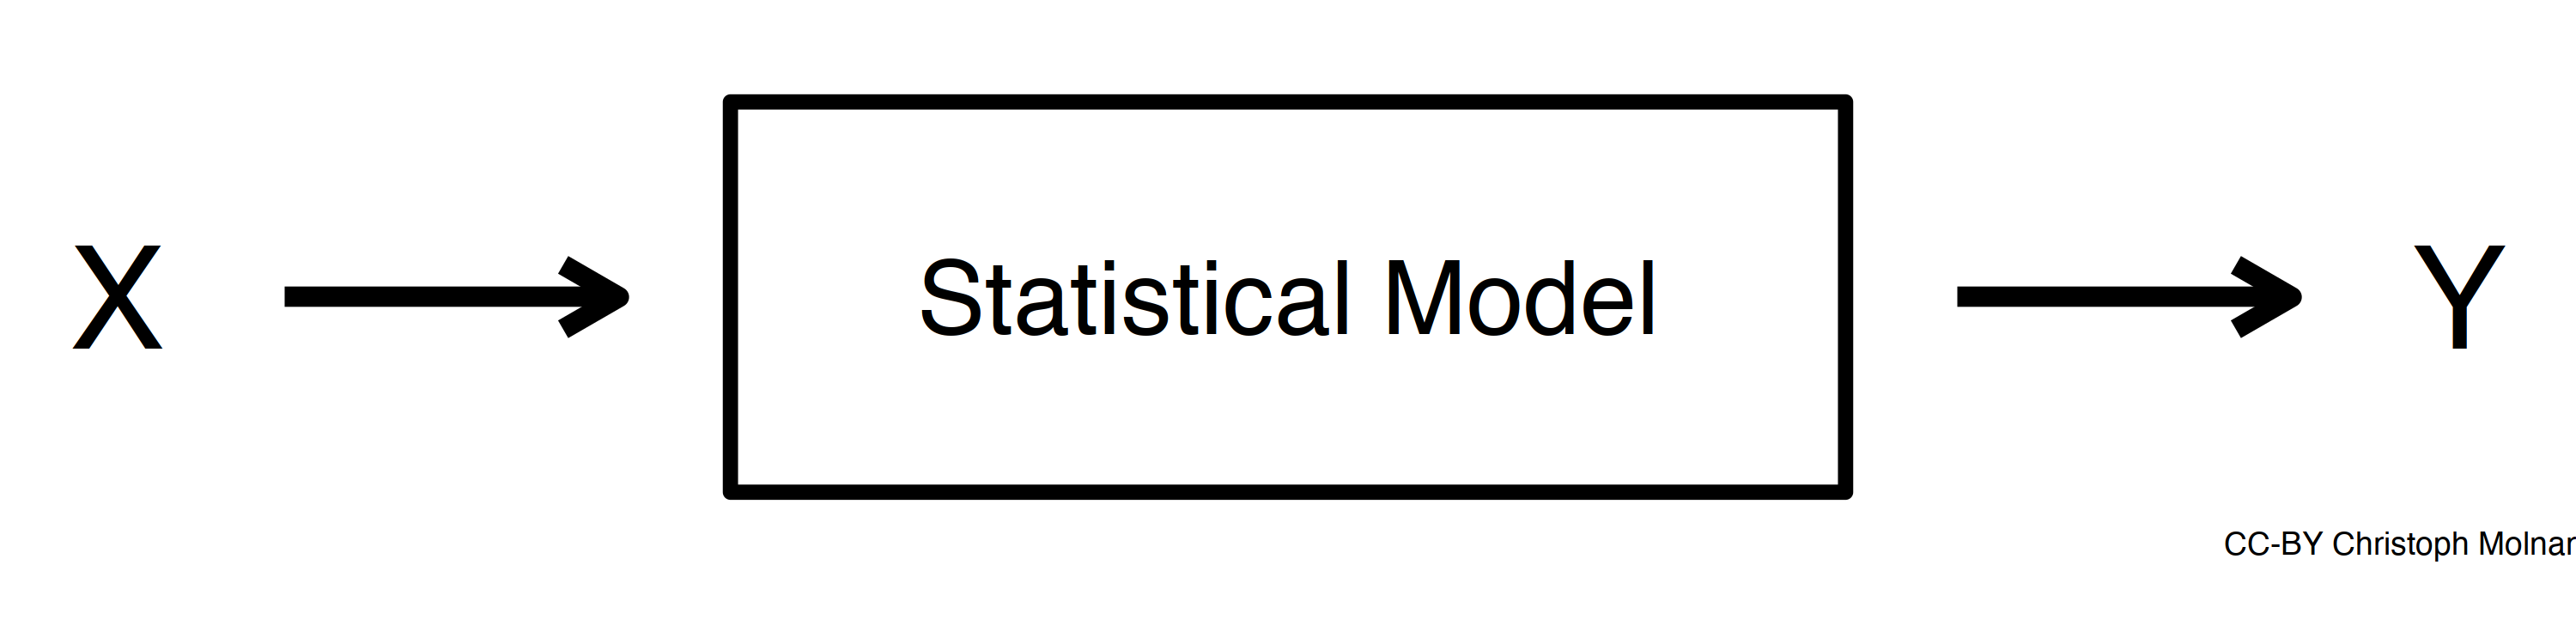
\includegraphics[width=0.8\textwidth]{figures/stats-1} 

}

\caption{Statistical Model}\label{fig:stats}
\end{figure}

In supervised machine learning, nature is seen as unknowable, or at least no attempt is even made to reverse-engineer the inner mechanisms of nature.
Instead of the intrinsic approach, supervised machine learning takes an extrinsic approach.
The supervised model is supposed to mimic nature.
It should show the same behaviour as nature, but it doesn't matter if it achieves this behaviour in the same way.

\begin{figure}

{\centering 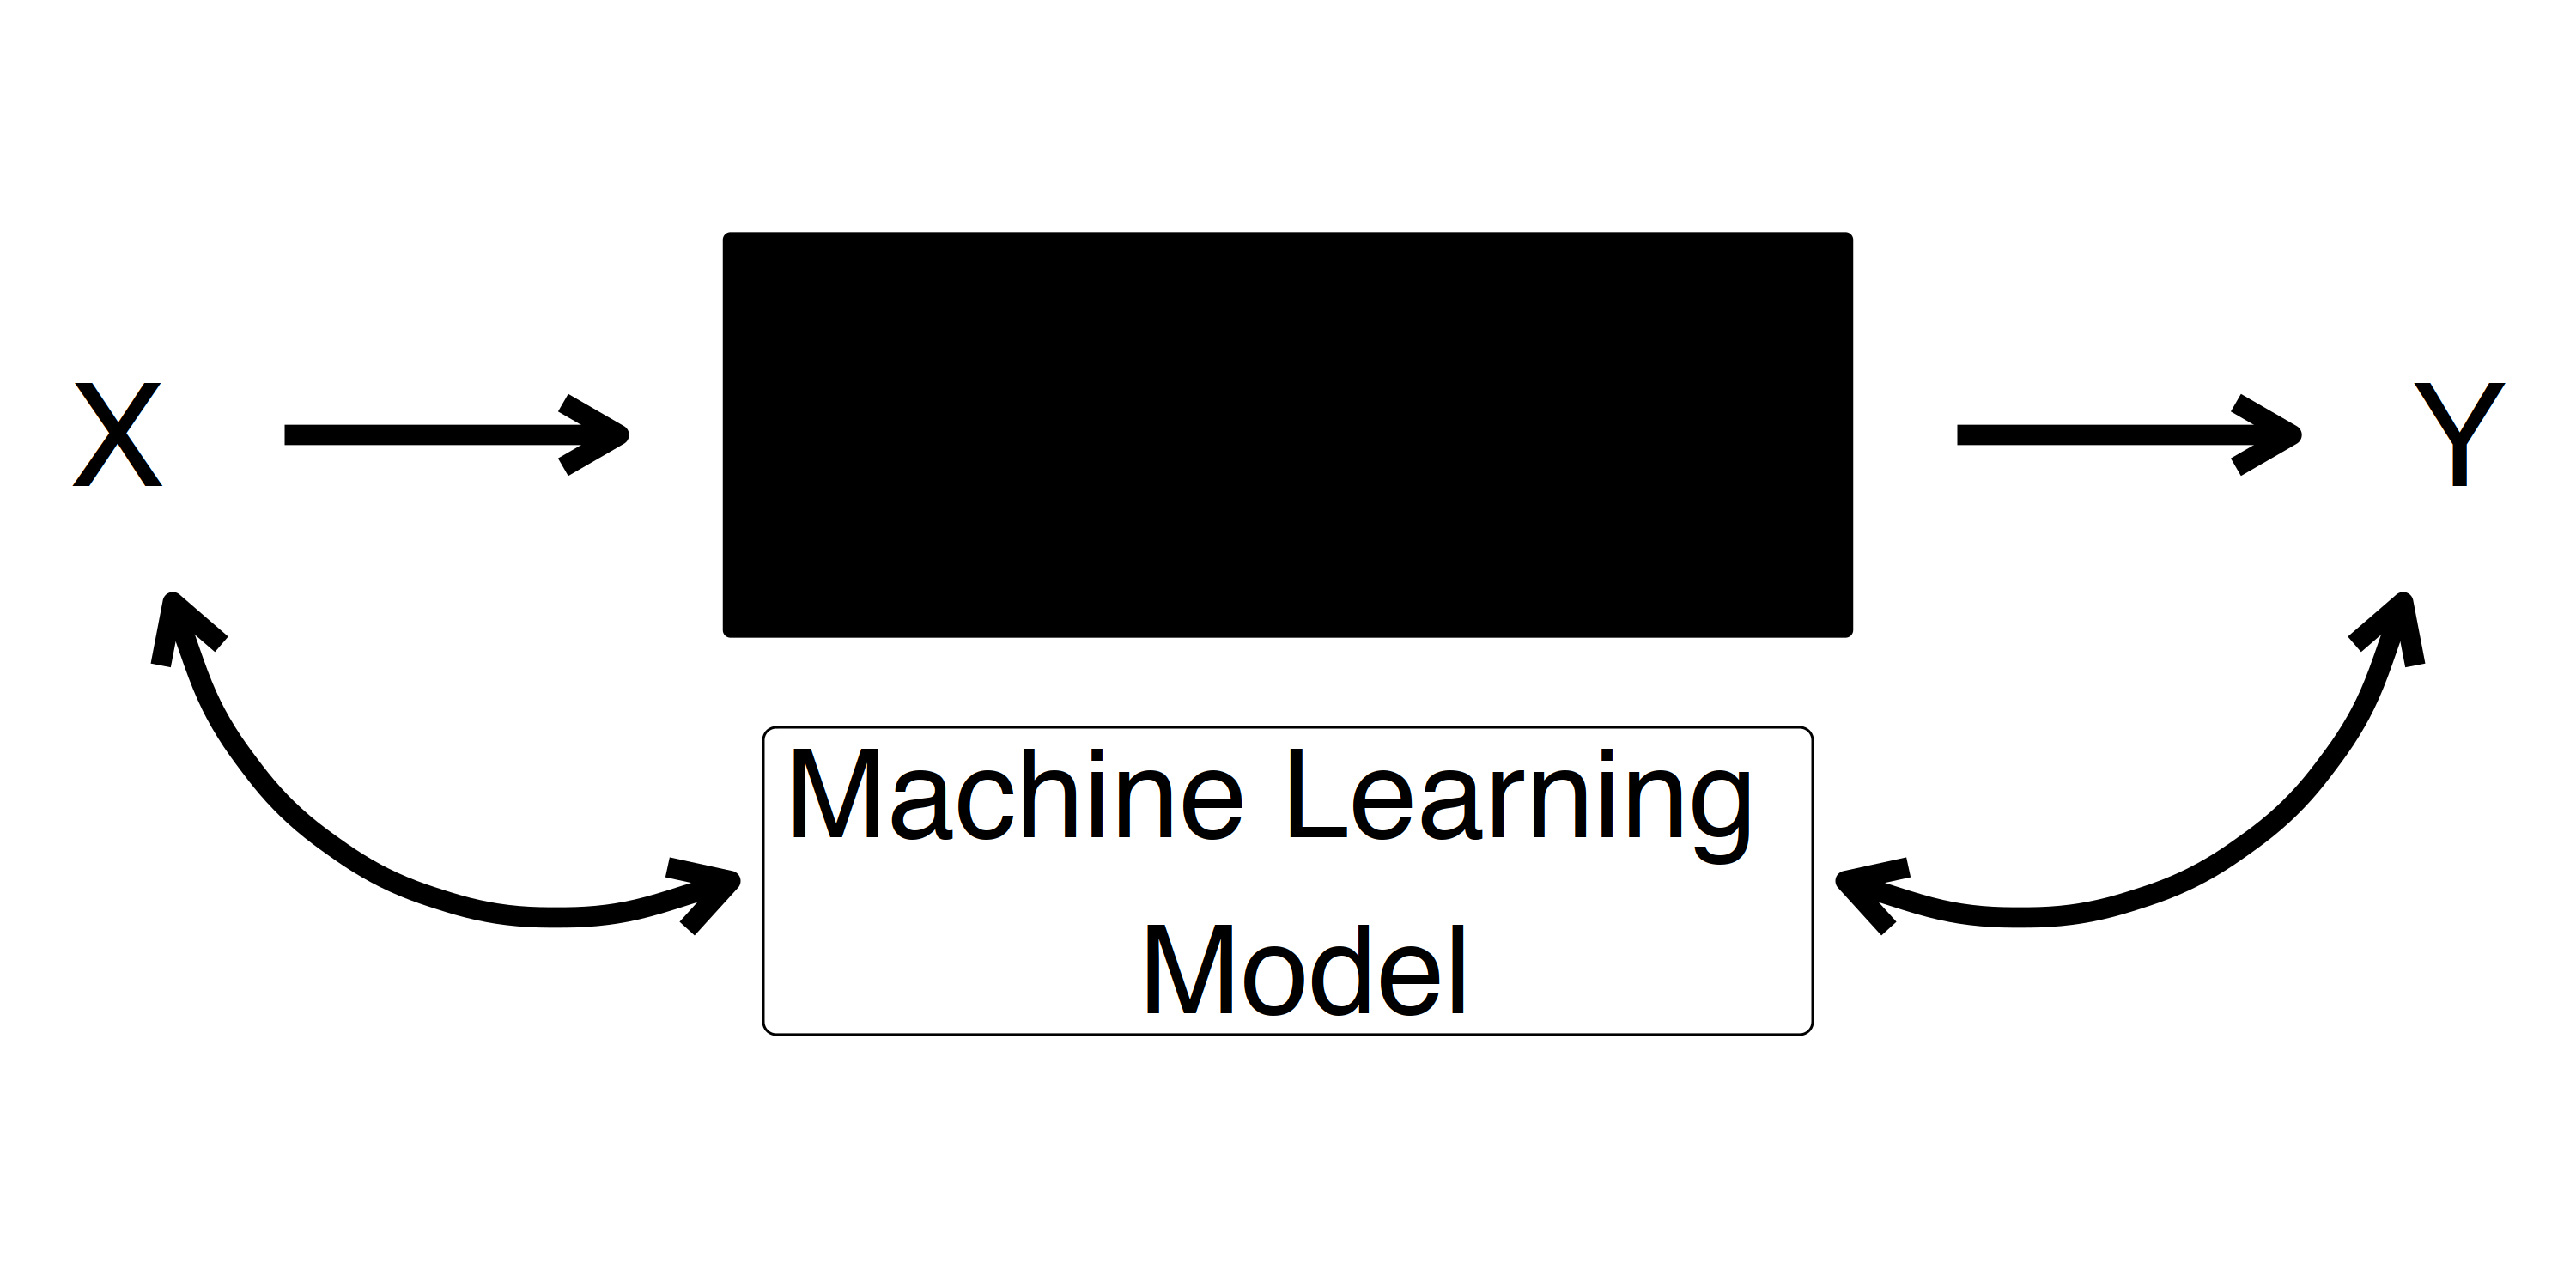
\includegraphics[width=0.8\textwidth]{figures/supervised-1} 

}

\caption{Supervised Machine Learning Model}\label{fig:supervised}
\end{figure}

Again, a cooking analogy:
Suppose you want to recreate a dish that you ate in a restaurant.
A statistician cook would try to find a plausible recipe, even if the end result is not perfect.
The supervised machine learner cook would only be interested in the end result;
it doesn't matter whether it's was exactly the same recipe.

No one mindset is inherently better or more useful than another.
They are different mindsets with different strengths and limitations.
If a task involves evaluating unseen data against a well-defined performance metric, the best approach to that task is probably supervised machine learning.
If your task requires a model with a strong theory that can explain the relationships in the data, statistical modeling is the way to go.

\hypertarget{strengths-6}{%
\section{Strengths}\label{strengths-6}}

\begin{itemize}
\tightlist
\item
  The most straightforward mindset when it comes to making predictions.
\item
  Loss function \(L\) allows the model to be adapted quite well to the task at hand.
\item
  Supervised machine learning is highly automatable.
\item
  Supervised learning has a very coherent evaluation approach that I personally find very convincing, though quite one-sided. Measuring how well the model predicts new data is a very compelling way to define a good model.
\end{itemize}

\hypertarget{limitations-6}{%
\section{Limitations}\label{limitations-6}}

\begin{itemize}
\tightlist
\item
  Supervised learning without constraints does not lead to interpretable models and is therefore not as well suited to for gaining insights.
\item
  Supervised learning is not as theoretically sound as statistical modeling.
\item
  Making decisions based on only the most likely outcome ignores tail risks from less likely, but possible extreme outcomes.
\item
  Uncertainty quantification is not a first class citizen as it is in, for example, \protect\hyperlink{bayesian}{Bayesian inference}. The modeler has to rely on a subset of machine learning algorithms that quantify uncertainty (for example Gaussian processes) or they have to use additional tools such as conformal prediction.
\item
  Automation can lead to overlooking issues with the data and the task formulation.
\item
  Generalization error is a good way to quantify generalization, relying solely on this metric will fail in the dumbest ways. There are many examples, such as using asthma as a predictor of lower risk of pneumonia\textsuperscript{\protect\hyperlink{ref-caruana2015intelligible}{20}}, classifying based on watermarks\textsuperscript{\protect\hyperlink{ref-lapuschkin2019unmasking}{21}}, and misclassifying dogs as wolfs based on snow in the background\textsuperscript{\protect\hyperlink{ref-ribeiro2016should}{22}}.
\item
  Feedback loops can break the models. Deployed into the wild, supervised learning models influences and even creates data that might end up training a future version of the same model. But this feedback loop is not well understood and difficult to respect in the modeling process.
\end{itemize}

\hypertarget{references}{%
\section{References}\label{references}}

\begin{itemize}
\tightlist
\item
  Statistical Modeling: The Two Cultures by Leo Breiman.\textsuperscript{\protect\hyperlink{ref-breiman2001statistical}{19}} Highly recommended to understand differences between statistical modeling and supervised machine learning.
\item
  I can recommend the book ``Elements of Statistical Learning''\textsuperscript{\protect\hyperlink{ref-hastie2009elements}{23}} which covers not only supervised learning but also other machine learning topics. The book has a strong influence from the statistical modeling mindset.
\end{itemize}

\hypertarget{unsupervised-ml}{%
\chapter{Unsupervised Learning}\label{unsupervised-ml}}

\begin{itemize}
\tightlist
\item
  A more open and diverse mindset focused on uncovering hidden patterns in the data.
\item
  Typical tasks: Clustering, anomaly detection, dimensionality reduction, and association rule learning.
\item
  One of the three \protect\hyperlink{machineux5cux2520learning}{machine learning} mindsets along with \protect\hyperlink{supervised-ml}{supervised learning} and \protect\hyperlink{reinforcement-learning}{reinforcement learning}.
\end{itemize}

A group of supervised learners and one unsupervised learner decide to climb a mountain.
The trip quickly turns into a race: Who will be the first to reach the top of the mountain, and who will be the first back to the hut?
The supervised learners try to outrun each other, one faster than the other.
The unsupervised learner quickly falls behind.
After an exhausting day, one by one, they return to their hut.
To their surprise, the unsupervised learner is already joyfully waiting for them in the hut.
Everyone was eager to know how the unsupervised learner managed to climb faster than them.
``When you all sprinted off, I took a detour,'' the unsupervised learner reported,``You won't believe this, but I found a rare mushroom that is not supposed to grow in this area. I have also divided the area around the hut according to the vegetation you find there. But the best part is that \ldots{}''
``Wait!'' interrupts one of the supervised learners, ``You were not only the first one back, but you also did all these other things?''
``I guess so'', the unsupervised learner admits, a little puzzled.
``How long did it take you to climb the mountain? Did you find a shortcut? We haven't seen you all day.'', asks another supervised learner.
``Mountain? I didn't see any mountains.''

\hypertarget{what-type-of-traveler-are-you}{%
\section{What Type of Traveler Are You?}\label{what-type-of-traveler-are-you}}

Tip Top Travel, a travel agency I just made up, offers a wide range of trips, from all-inclusive holidays in Spain to hiking trips in Norway and weekend city trips to Paris.
They have a huge database on the booking history of their customers:
The date of the trip, the destination, group size, cost of the trip, and so on.
And yet, they know surprisingly little about the general patterns in their data:
Are there certain prototypes of customers?
Do customers who book trips to Norway, for example, also book trips to Sweden?
Our imaginary travel company's big data is a dream for unsupervised learners.
They might start with a cluster analysis to get an overview Tip Top Travel's different customer types.
A cluster is a group of customers with similar travel patterns.
Similar means that the customers in a cluster are ``close'' in terms of their feature values, such as booking frequency, travel locations, and average cost of the trip.
If Tom books 4 trips per year, he is more similar to Tina, who books 5 trips per year than Philipp, who books 1 per year.
It gets more tricky because the measure of distance between travelers has to combine features that were measured at very different scales, such as amount of money, geographical location, counts, and so on.
But I'll rant about that problem later.
With such a distance measure, there are many clustering algorithms to choose from that can detect clusters.
For example, the k-means algorithm.

\begin{figure}

{\centering 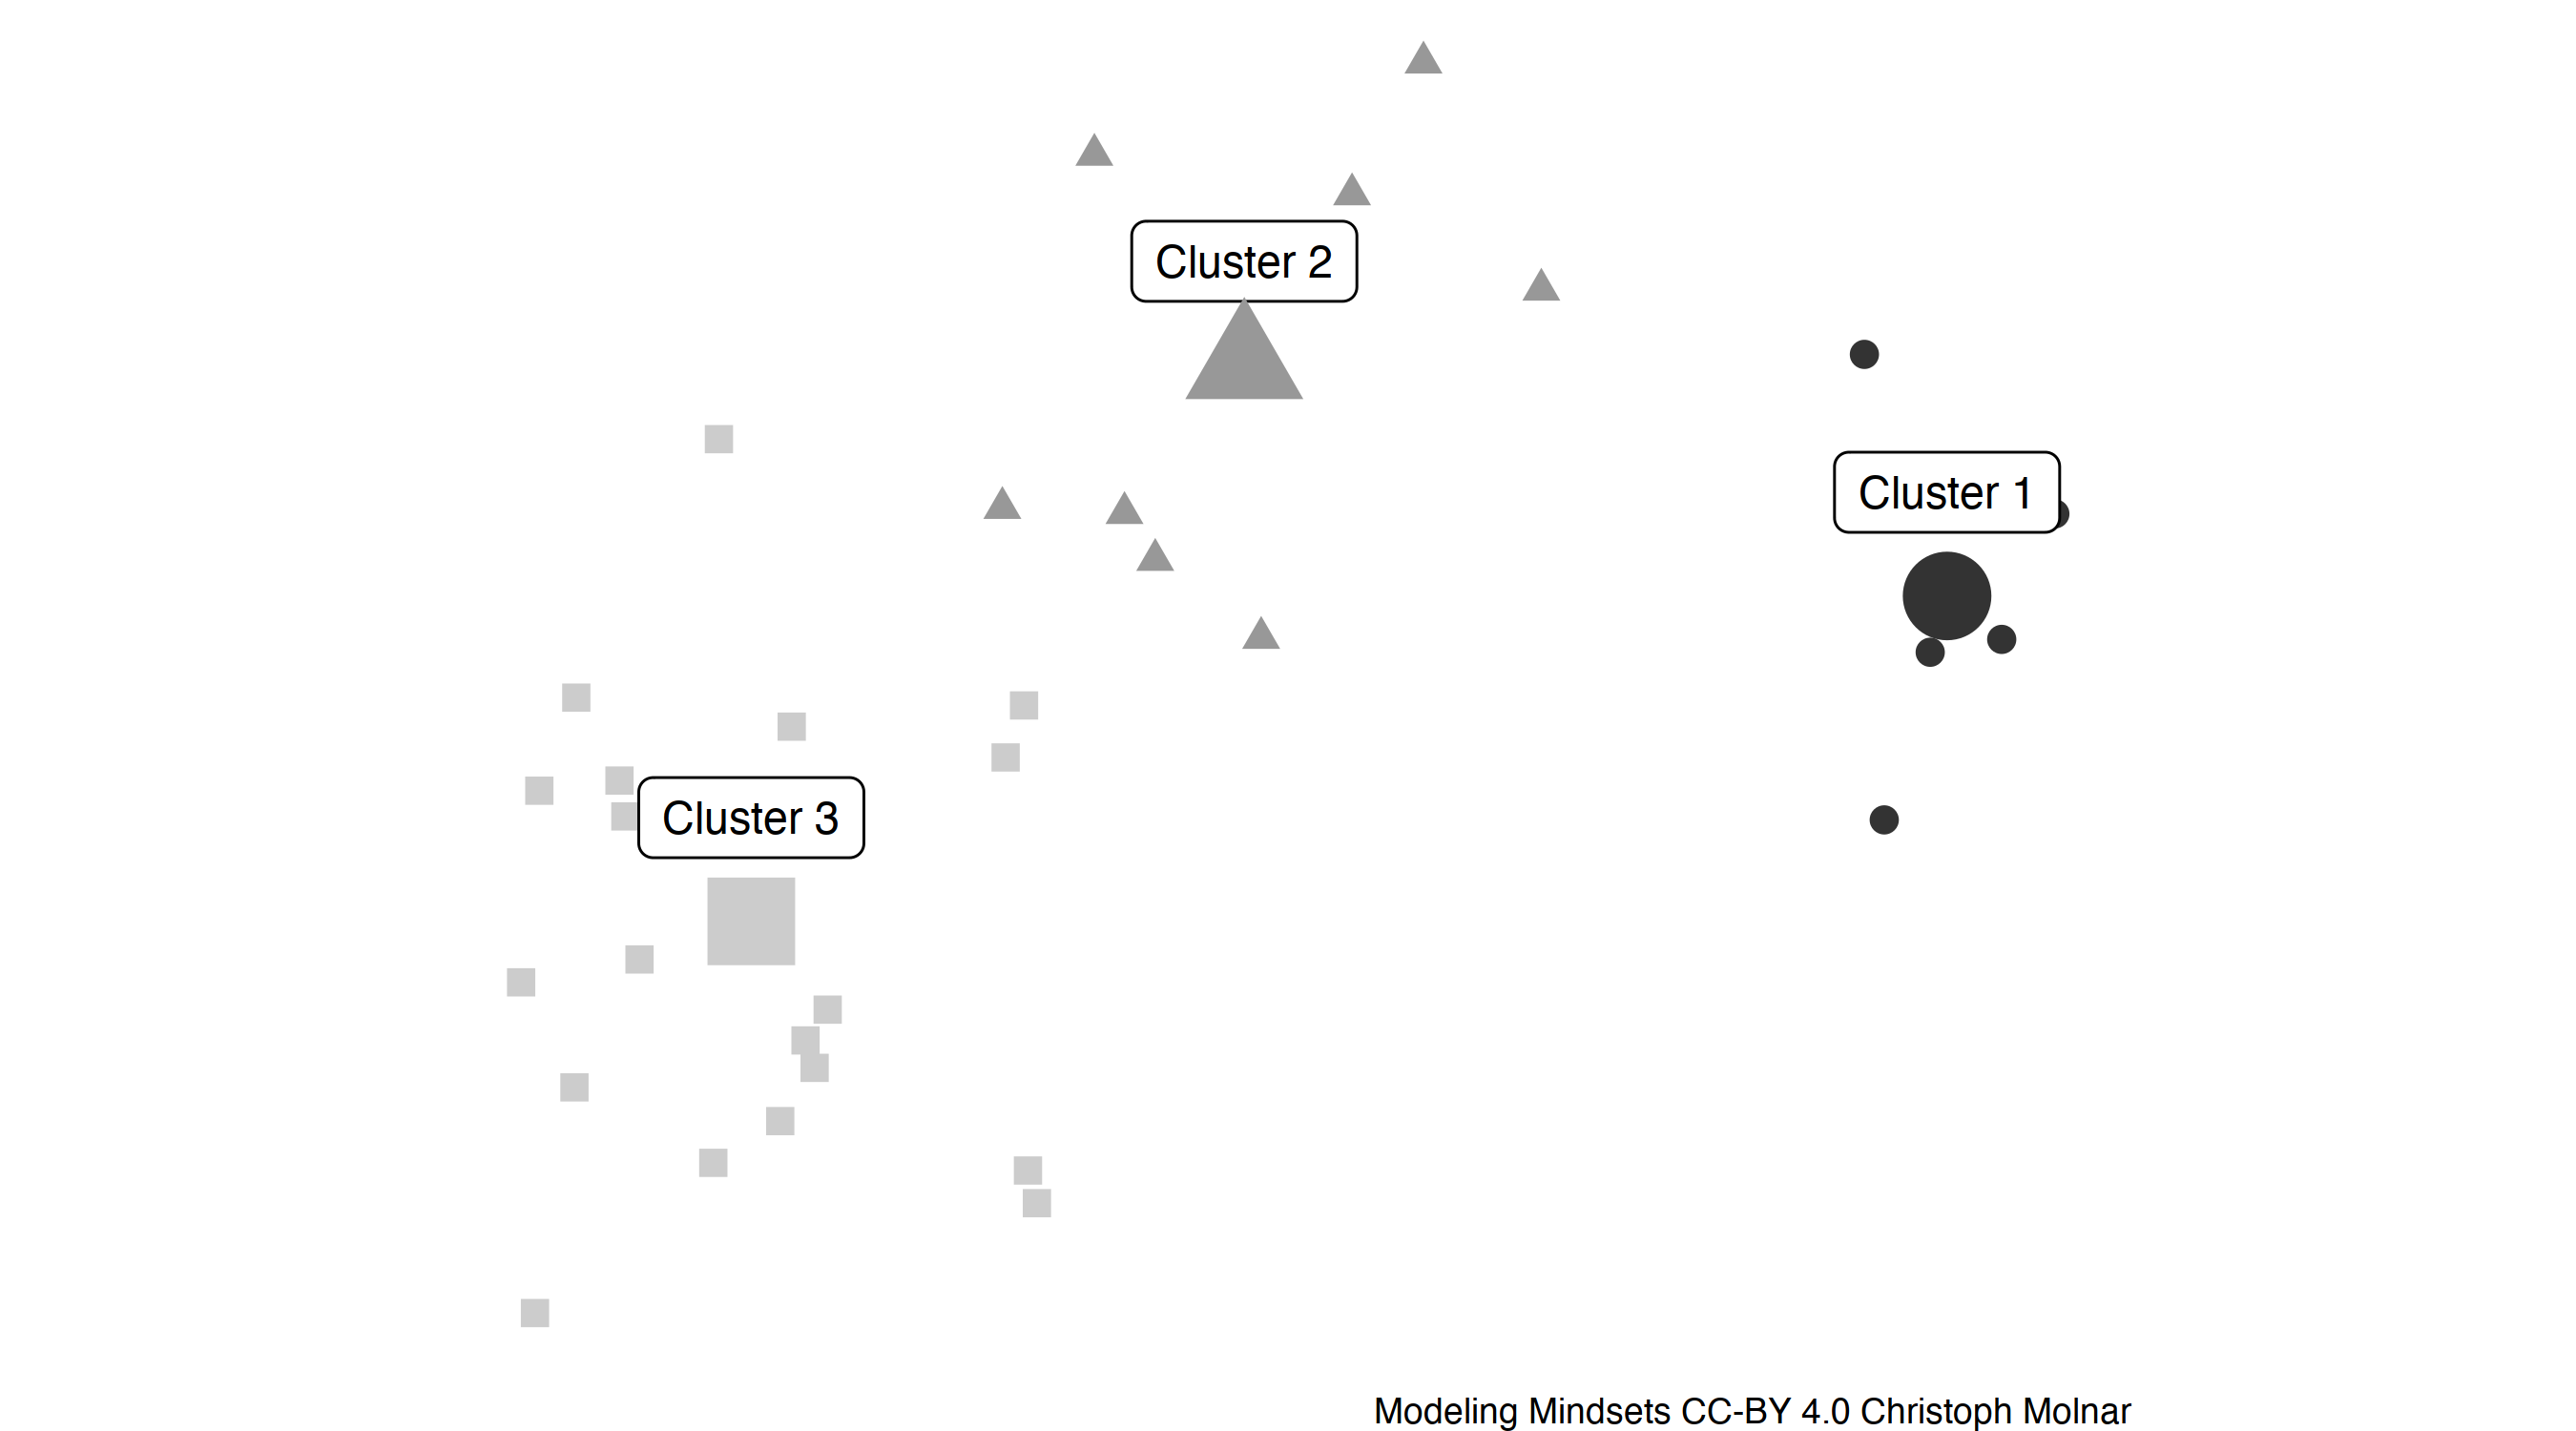
\includegraphics[width=0.8\textwidth]{figures/clustering1-1} 

}

\caption{Three clusters for two features (x-axis and y-axis) based on k-means clustering.}\label{fig:clustering1}
\end{figure}

The k-means algorithm divides our customers into \(k\) clusters.
The number of clusters \(k\) must be chosen by the modeler.
The algorithm start with random cluster centers.
These cluster centers are iteratively optimized so that all customers in the same cluster are close to each other.
Each customer is assigned to the cluster with the closest center.
The objective of the k-means algorithm is to find cluster centers that minimize the distances between centers and assigned data points, averaged over all customers.

Great! We have clusters.
Now what?
We wanted to know what kind of customers Tip Top Travel has.
To do this, we can interpret the cluster centers as prototypes of customers.
One cluster could be ``families looking for relaxation''.
The cluster center is a customer that books about twice a year for 1.9 adults and 2.1 children.
The most common destination is all-inclusive hotels with pool and beach access, where parents can drop off their kids for an all-day entertainment program and then the adults can have their first beer at the pool bar 11 AM.
Cluster numero dos is ``luxury explorer''.
Customers in this cluster book an average of 0.7 trips per year for 1.7 adults, with varying destinations in nature with some adventure aspect: hiking, canoeing and camping.
Depending on the \(k\) chosen by the modelers, there might be more clusters, and they might not always map to some easily interpretable group of travelers.
The more interpretable the clusters are, the more the marketing department will love the results.
Cluster analysis can provide data-driven insights about customers and offers a narrative angle on which to build marketing campaigns.

\hypertarget{the-unsupervised-learning-mindset}{%
\section{The Unsupervised Learning Mindset}\label{the-unsupervised-learning-mindset}}

Unsupervised learning is like a journey of discovery.
A dataset suddenly becomes a treasure chest potentially filled with valuable insights.
The supervised learner can only watch from the sidelines: sipping an energy drink, preparing for the next race; the only excitement is what the stopwatch will show this time.

Unsupervised learning is a machine learning mindset: task-driven, computer-oriented, and externally motivated.
Task-driven: We use unsupervised learning to solve specific tasks, such as clustering, anomaly detection, or finding a better representation of the data.
Computer-oriented: Like supervised learning, its unsupervised counterpart is motivated by the premise of having a computer, rather than by the premise of a theory where it's simply convenient to have a computer.
Unsupervised learning is externally motivated: While measuring performance is more difficult than in other machine learning mindsets, successfully completing the task is more important than following a particular ``recipe'' (such as using probability theory).

Unsupervised learning is a less coherent mindset than supervised learning with its very rigorous evaluation and Zen-like mindset of optimization.
Unsupervised learning is about discovering patterns in the data, which sounds a bit fuzzy.
Fortunately, we can use the language of probability theory to make it more understandable.
Unsupervised learning is about finding a more compact representation of the joint distribution \(P(X)\) or revealing some aspects of \(P(X)\).
Unsupervised learning includes a broad range of tasks:

\begin{itemize}
\tightlist
\item
  Clustering finds modes of the distribution.
\item
  Anomaly detection finds extreme data points.
\item
  Association rule learning finds modes in binary feature distributions.
\item
  Dimensionality reduction finds lower-dimensional descriptions of the data.
\item
  \ldots{}
\end{itemize}

Why do we need unsupervised learning anyway?
Can't we just hire a statistician to estimate \(P(X)\) and derive all these interesting aspects from that estimate?
Well, estimating the joint distribution is extremely difficult with high-dimensional data.
The difficulties in estimating \(P(X)\) become difficult even with more than a handful of features when the distribution is complex, let alone image or text data.

We can also express supervised learning as learning a distribution.
But it's ``only'' the conditional distribution \(P(Y|X)\), which is much easier to learn than the full joint distribution \(P(X)\).
Supervised learning is about selecting one feature and making it ``special'', which we also express by giving it a different letter (\(Y\)).
In unsupervised learning, on the other hand, all features are treated the same.
Of course, each algorithm can give different weights to the features depending on the task.

The lack of a target \(Y\) to predict also means we have no ground truth to compare our results to.
It's more like, ``Here are \(n\) data points, please find something interesting.''
Then you say ``Here's something interesting: I found these 10 clusters.''
But you'll never get any feedback on whether these were the ``right'' clusters.
There is no one to pat you on the back and say ``You did a great job.''
Your strength as an unsupervised learner must come from within!
That's why unsupervised learning is sometimes called learning without a teacher:
There is not teacher to correct the model.
This is also why we can clearly distinguish supervised learning as its own mindset and why it's not just a special case of unsupervised learning.

To be more cheerful about unsupervised learning:
It's, in many ways, an open mindset.
Unsupervised learning means being open to surprises and discovering hidden patterns.
The word ``pattern'' hides a potpourri of meanings: clusters, outliers, feature representations, association rules, \ldots{}
The mindset is also open in the sense that the range of methods is huge, even for a machine learning mindset.
For clustering alone, there are so many different approaches.
If I had to pick one modeling mindset that is the most inclusive, I would choose unsupervised learning (in terms of methods, not necessarily people).
Next to this hippie community, supervised learners look like dull optimizers who sit in their offices with fine suits trying to increase sales for the second quarter.

Full disclosure: unsupervised learning also involves optimization.
But there is much more freedom in the optimization objective because there is no ground truth.
The same is true for performance metrics and benchmarks:
It's part of the mindset to evaluate models, but there's a lot of ambiguity about how to evaluate unsupervised solutions.
For example, in cluster analysis, we could measure cluster purity, the silhouette score, various indexes, look at elbow plots, and so on.
One can also create a long list of metrics for supervised learning, but at least they agree on when they become zero (or reach their minimum):
When the target is accurately predicted.
A luxury that doesn't exist in unsupervised learning.

\hypertarget{many-tasks}{%
\section{Many Tasks}\label{many-tasks}}

To get a better understanding of unsupervised learning, let's take a look at some of the tasks that are typical of the mindset.

\hypertarget{clustering-and-outlier-detection}{%
\subsection{Clustering and Outlier Detection}\label{clustering-and-outlier-detection}}

Both clustering and outlier or anomaly detection are two opposites sides of the same coin.
In both cases, the question is where the mass of the data lies.

\begin{figure}

{\centering 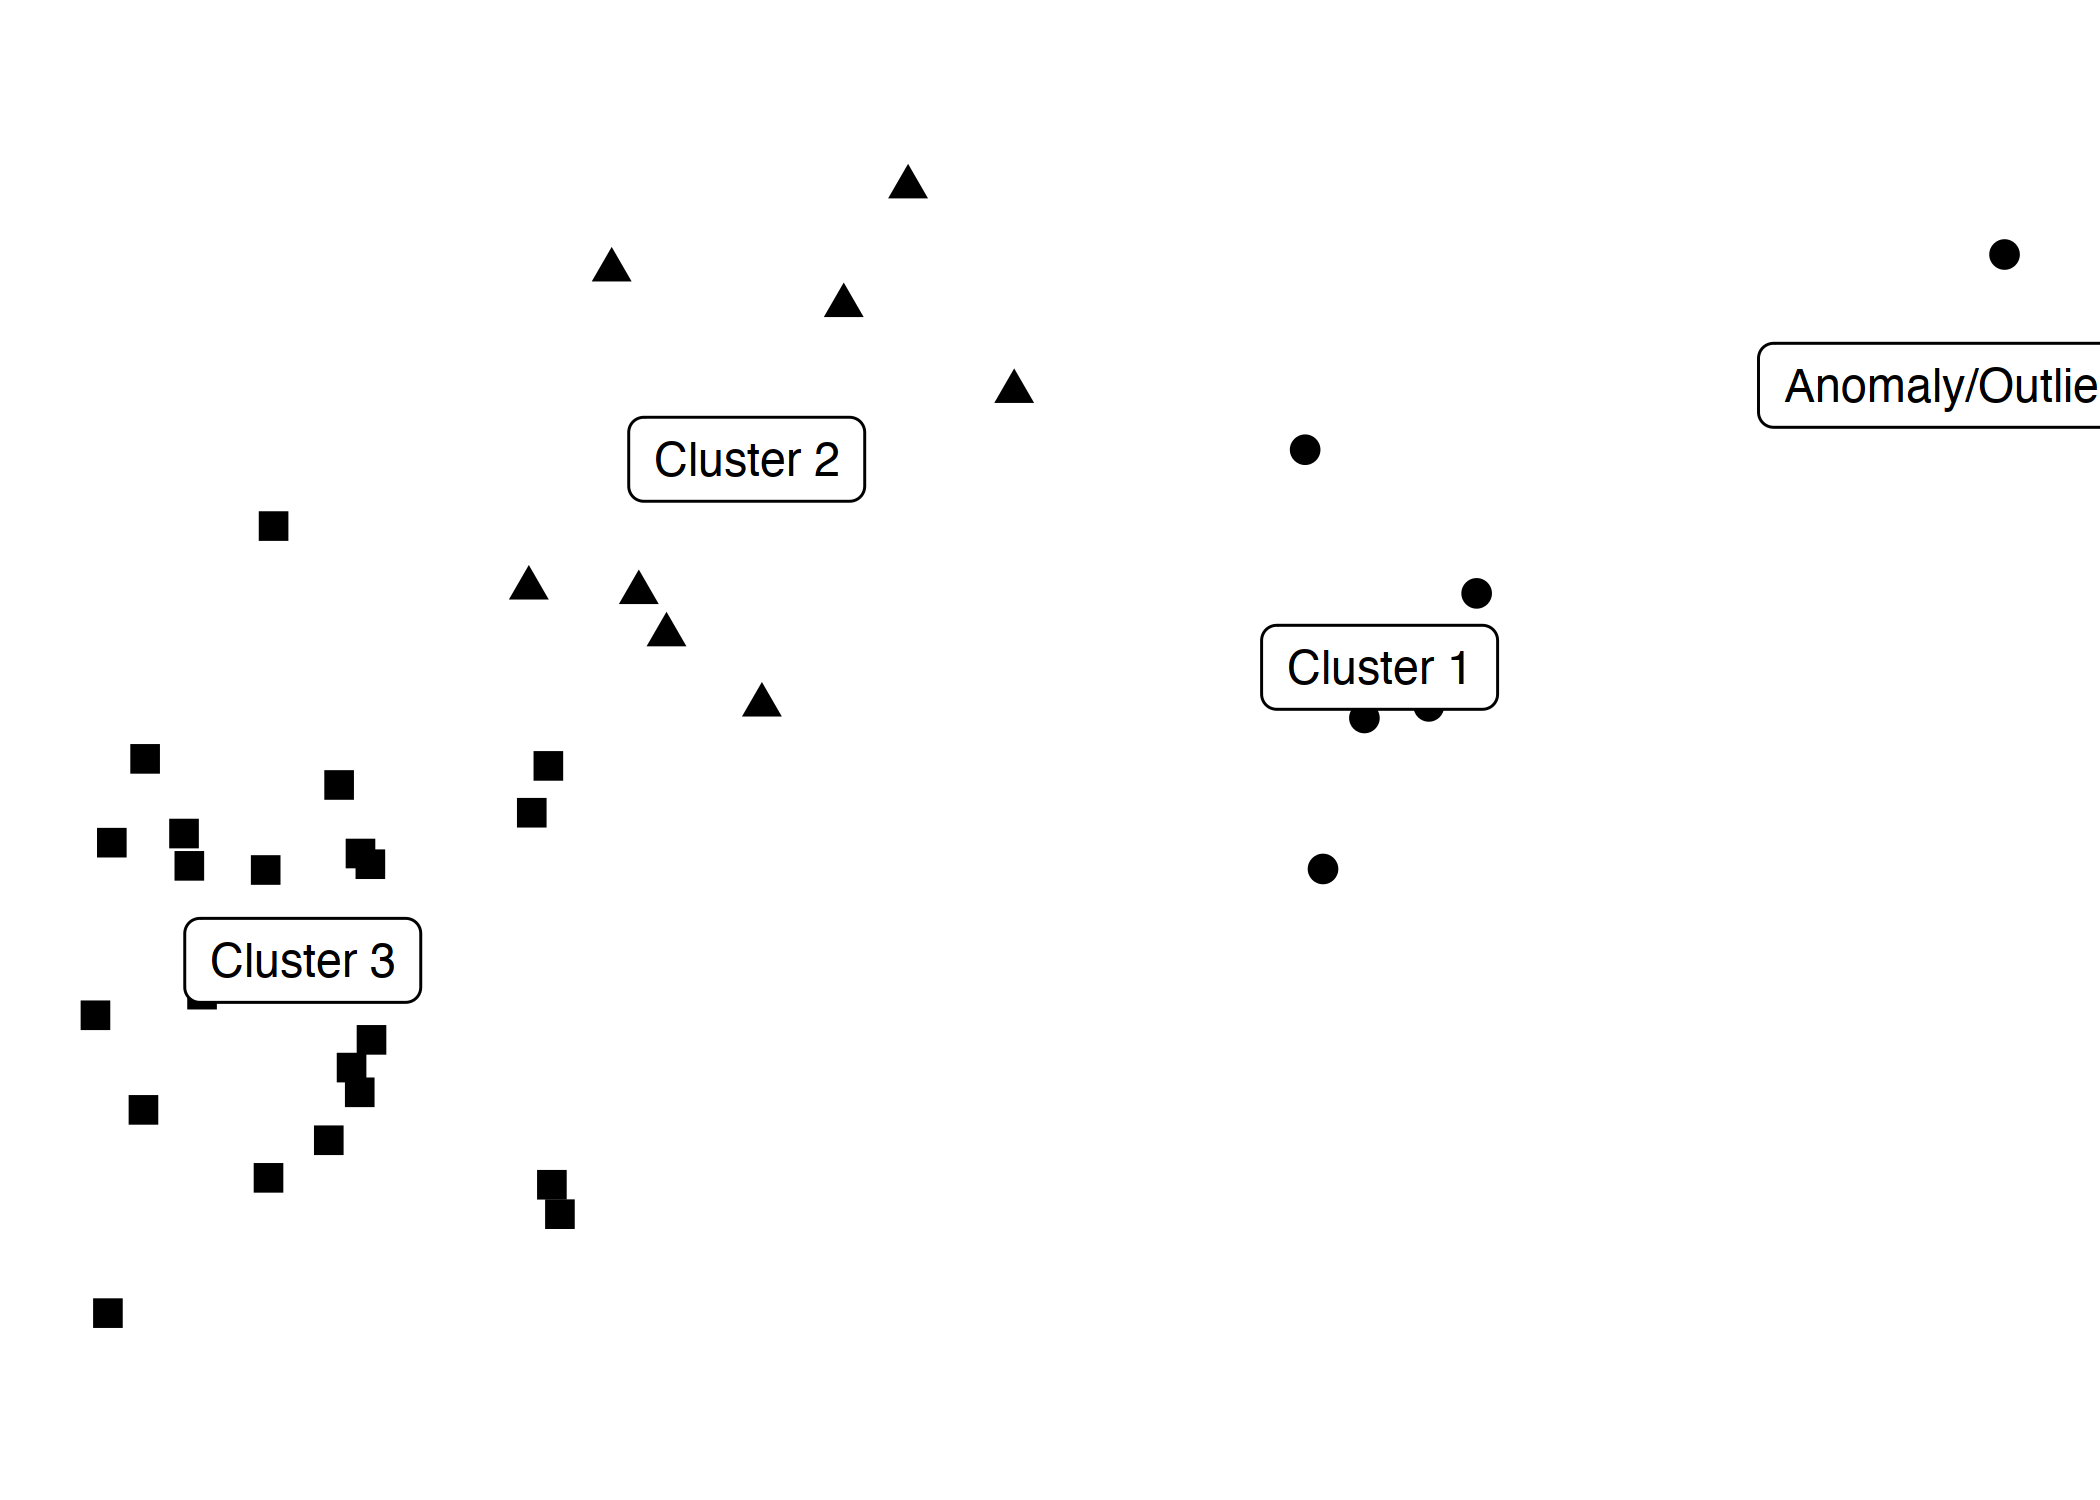
\includegraphics[width=0.8\textwidth]{figures/clustering-1} 

}

\caption{Example of three clusters in a two-dimensional feature space. The data point on the top right could be called an outlier.}\label{fig:clustering}
\end{figure}

Clusters are regions in the feature space with a high concentration of data points.
In terms of \(P(X)\), these regions are modes of the distribution.
Outliers or anomalies are in regions where \(P(X)\) is small, which are regions in the feature space with almost no data points.
Clusters are usually defined such that all the data points within a cluster a similar in their feature values.
There are many different approaches for finding clusters: hierarchical clustering, k-means, k-medoids, DB-SCAN, PRIM, Gaussian mixture models, self-organizing maps, \ldots{}
These clustering methods have various motivations, ranging from statistical to more algorithmic, again showing that unsupervised learning is externally motivated:
It isn't particularly important \emph{how} the clusters are detected.
Different clustering methods can find very different clusters.
Let's take a look at a another solution for cluster analysis from Figure \ref{fig:clustering1}.

\begin{figure}

{\centering 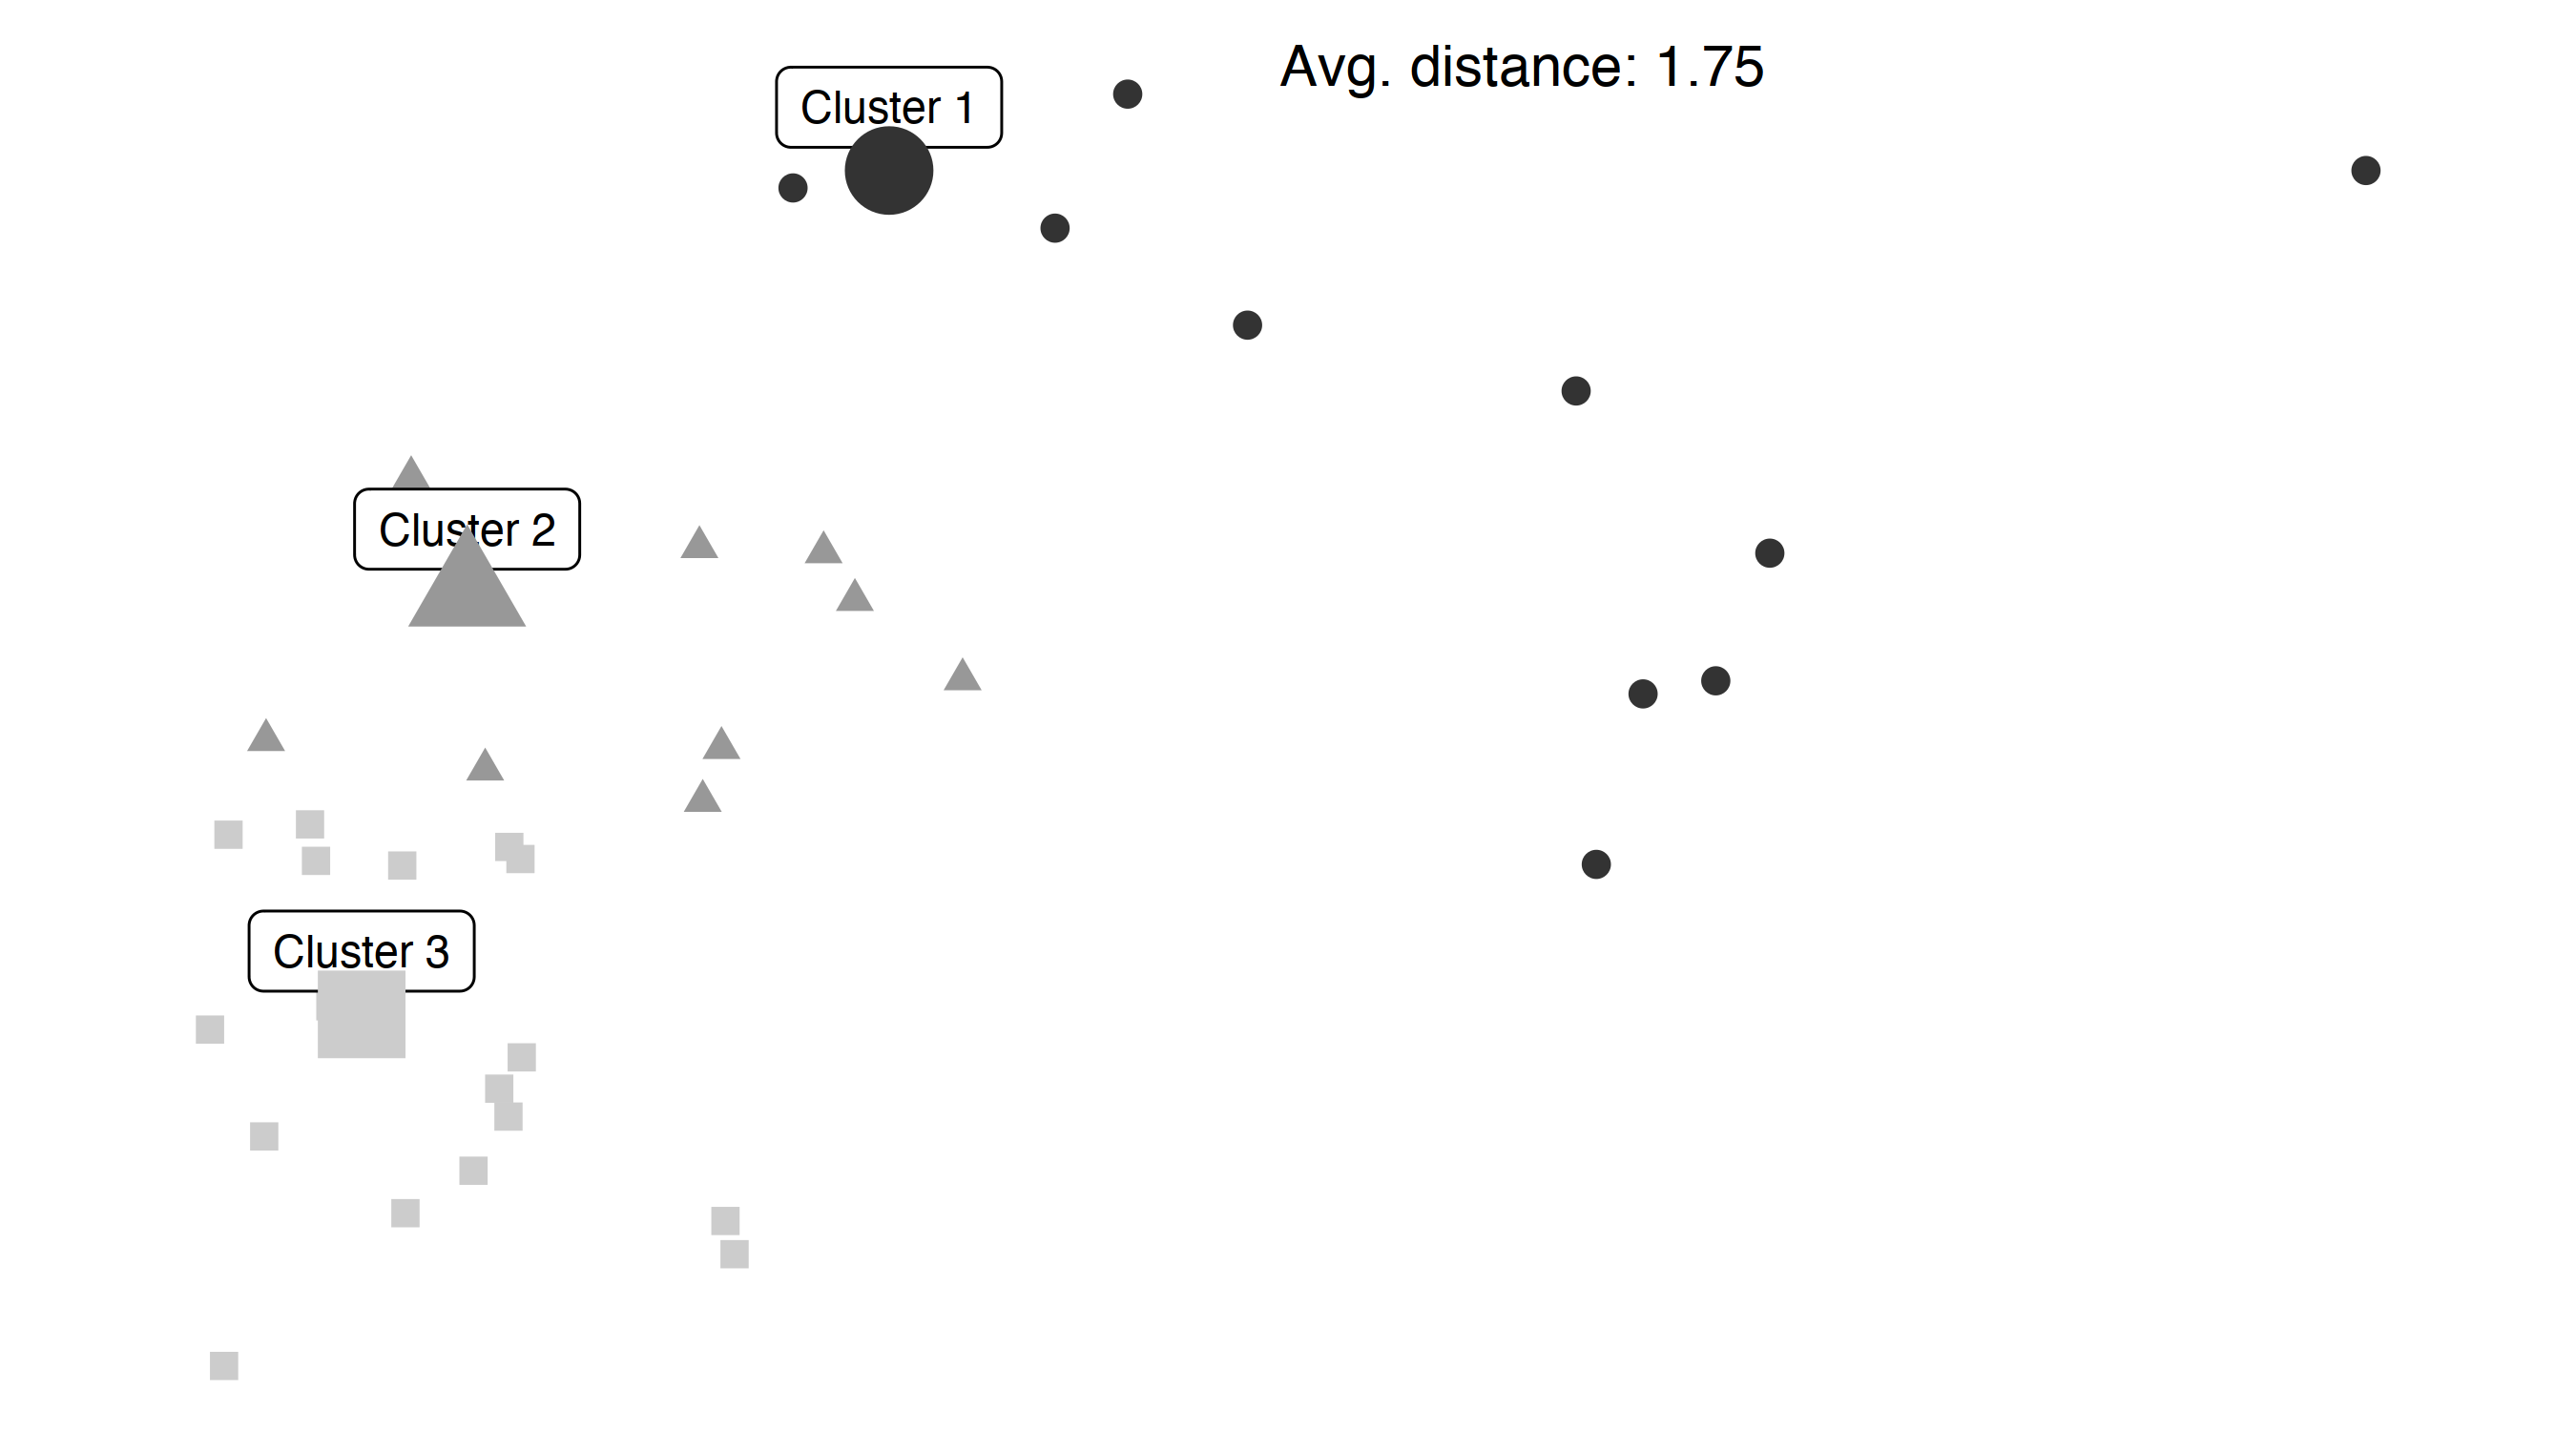
\includegraphics[width=0.8\textwidth]{figures/clustering2-1} 

}

\caption{Bad clustering solution, measured by Euclidean distance. But good solution if we are only interested in the horizontal direction, giving a weight of zero to the feature that distributes the data in the vertical direction.}\label{fig:clustering2}
\end{figure}

The clusters in Figure \ref{fig:clustering2} are clearly a poor solution based on Euclidean distance.
But this assumes that both features matter are equally important for computing similarity.
Perhaps the feature that spreads the data in the horizontal direction is rather irrelevant, and we want to give it less weight in the distance computation?
Domain experts can tell you which features are important and which aren't.
Usually, all features are weighted equally, which seems to be a sensible decision at first glance.
But in truth, any other weighting can an equally good choice.
For example, when clustering fruits, two of the features might be highly correlated:
We could use the features ``volume'' and ``volume after peeling''.
In practice, we now have two features with almost the same information.
If we use both of the feature for clustering, it's as if we give twice as much weight to the volume of the fruit as to any other feature.

And it gets worse.
What do we do when features are measured at different scales, such as a weight, a length, and a sum of money?
How can we even combine these features into a single distance measure, especially when the features even have different cardinalities, like numerical and categorical features?

``Excuse me, how do I get from point A to point B?''
``You go down this street and turn right after 10 meters. Then you go another \$7 and turn left until red becomes blue!''.
And also, what's closer to a banana? An apple or a lemon?
Sounds almost like an obscure interview question for a data scientist position at large web search company.
But it's a question you better have some answers to if you do cluster analysis.

So no one can tell you what's right.
As an unsupervised machine learner, you have to live with ambiguity.
Going to bed every night, questioning the fabric of space and time.
Supervised machine learners don't have this problem, at least not to this extent.
The weighting of features is ``supervised'' by the relationship between the features and the target for which we know the ground truth.

\hypertarget{anomaly-detection}{%
\subsection{Anomaly Detection}\label{anomaly-detection}}

Cybersecurity specialists monitor events in the intranet.
Their job is to protect the company from cyber threats: Trade secret theft, malware, digital blackmail, you name it.
But there are thousands of employees who leave their digital footprint every day.
A mass, or rather, mess of data.
What does an attack look like?
The specialist has rules to detect some forms of attacks:
If someone tries to brute force a password to log into a service, that's a red flag.
But what about all the behaviors that don't follow such simple patterns, perhaps even unknown type of attacks?
Fortunately for the cybersecurity specialist, there is unsupervised learning.
Anomaly detection, an unsupervised learning task, is concerned with finding extreme data points.
Typical applications include financial fraud detection and cybersecurity.
Isolation forests, a popular anomaly detection tool, instead work by isolating data points that are extreme.
Other algorithms are directly motivated by probability distributions and flag data points as anomalies if they have a low probability.
Isolation forests, statistical tests, but also one-class support vector machines and hidden Markov models -- the variety of methods shows yet again that machine learning, in this case unsupervised, is a very pragmatic modeling mindset.

\hypertarget{association-rule-learning}{%
\subsection{Association Rule Learning}\label{association-rule-learning}}

I love grocery shopping.
Many people hate it, but only because they are unaware of it's magnificence:
Supermarkets are incredible places that deserve awe and wonder and embody the progress and ingenuity of humanity.
Supermarkets are like the land of milk and honey.
It's incredible what you can get in the supermarket: exotic fruits, spices from all over the world, products that take months or even years to make, like soy sauce, wine and cheese.
But I digress.
Let's talk about association rule learning, which is usually introduced with shopping baskets as example.
When you go shopping, you can think of your shopping basket as a binary dataset.
Either you buy a certain item (1) or you don't buy it (0).
Other people also go shopping and generate their own data of 0's and 1's.

The baskets might look like this: \(\{yeast, flour, salt\}\), \(\{beer, chips\}\), \(\{sandwich, lemonade, chips\}\), \(\{cheese, onions, tomatoes, potatoes, flour, olive oil, chocolate, beer, chips\}\).
The goal of association rule learning is to detect the patterns of items.
Do people who buy flour often buy yeast?
Association rule mining is again a case of describing \(P(X)\).
An association rule might be \(\{beer\} \Rightarrow \{chips\}\) and would mean that people who buy beer frequently buy chips.
In more formal terms, association rules are short descriptions that use conjunctive rules to describe high density regions in a binary feature space.
A well-known algorithm is the Apriori algorithm, but again, there are many option to choose from.
The next time you go to the supermarket, please take a moment.
Take it all in.
The fact that you have so many choices.
Many bad things are happening in the world, but when you stand in a supermarket (with enough money), you are living what humanity must have dreamed of for thousands of years and what we take for granted.
I hope you appreciate this as much as I do.

\hypertarget{dimensionality-reduction}{%
\subsection{Dimensionality Reduction}\label{dimensionality-reduction}}

Unfortunately, there is the ``curse of dimensionality''.
The curse is that data density decreases exponentially with each additional features.
If the number of data points remains constant, adding more features makes any modeling task more difficult, regardless of the mindset.
Dimensionality reduction can be used to break this curse, or at least reduce its burden.
If unsupervised learning regards all features, on what basis can we reduce the dimensionality?
Not all features contribute towards \(P(X)\).
Some features may almost have no variance.
Other features may be highly correlated with other features.
In either case, we can select a subset of the features, and \(P(X)\) will mostly look the same.
There are several methods for feature selection based on information-theoretic measures such as statistical correlation.

Or we can take our data and map it into a lower-dimensional space.
Those dimensionality reduction techniques usually make you wish you had paid better attention in linear algebra.
They can usually be represented as matrix multiplication of your original feature matrix: principal component analysis (PCA), ICA, non-negative matrix factorization, multidimensional scaling, t-SNE, and so on.
If each of your data point represents a fruit, features like height, width and weight could be mapped to a new feature / dimension that represents the volume of the fruit.

\begin{figure}

{\centering 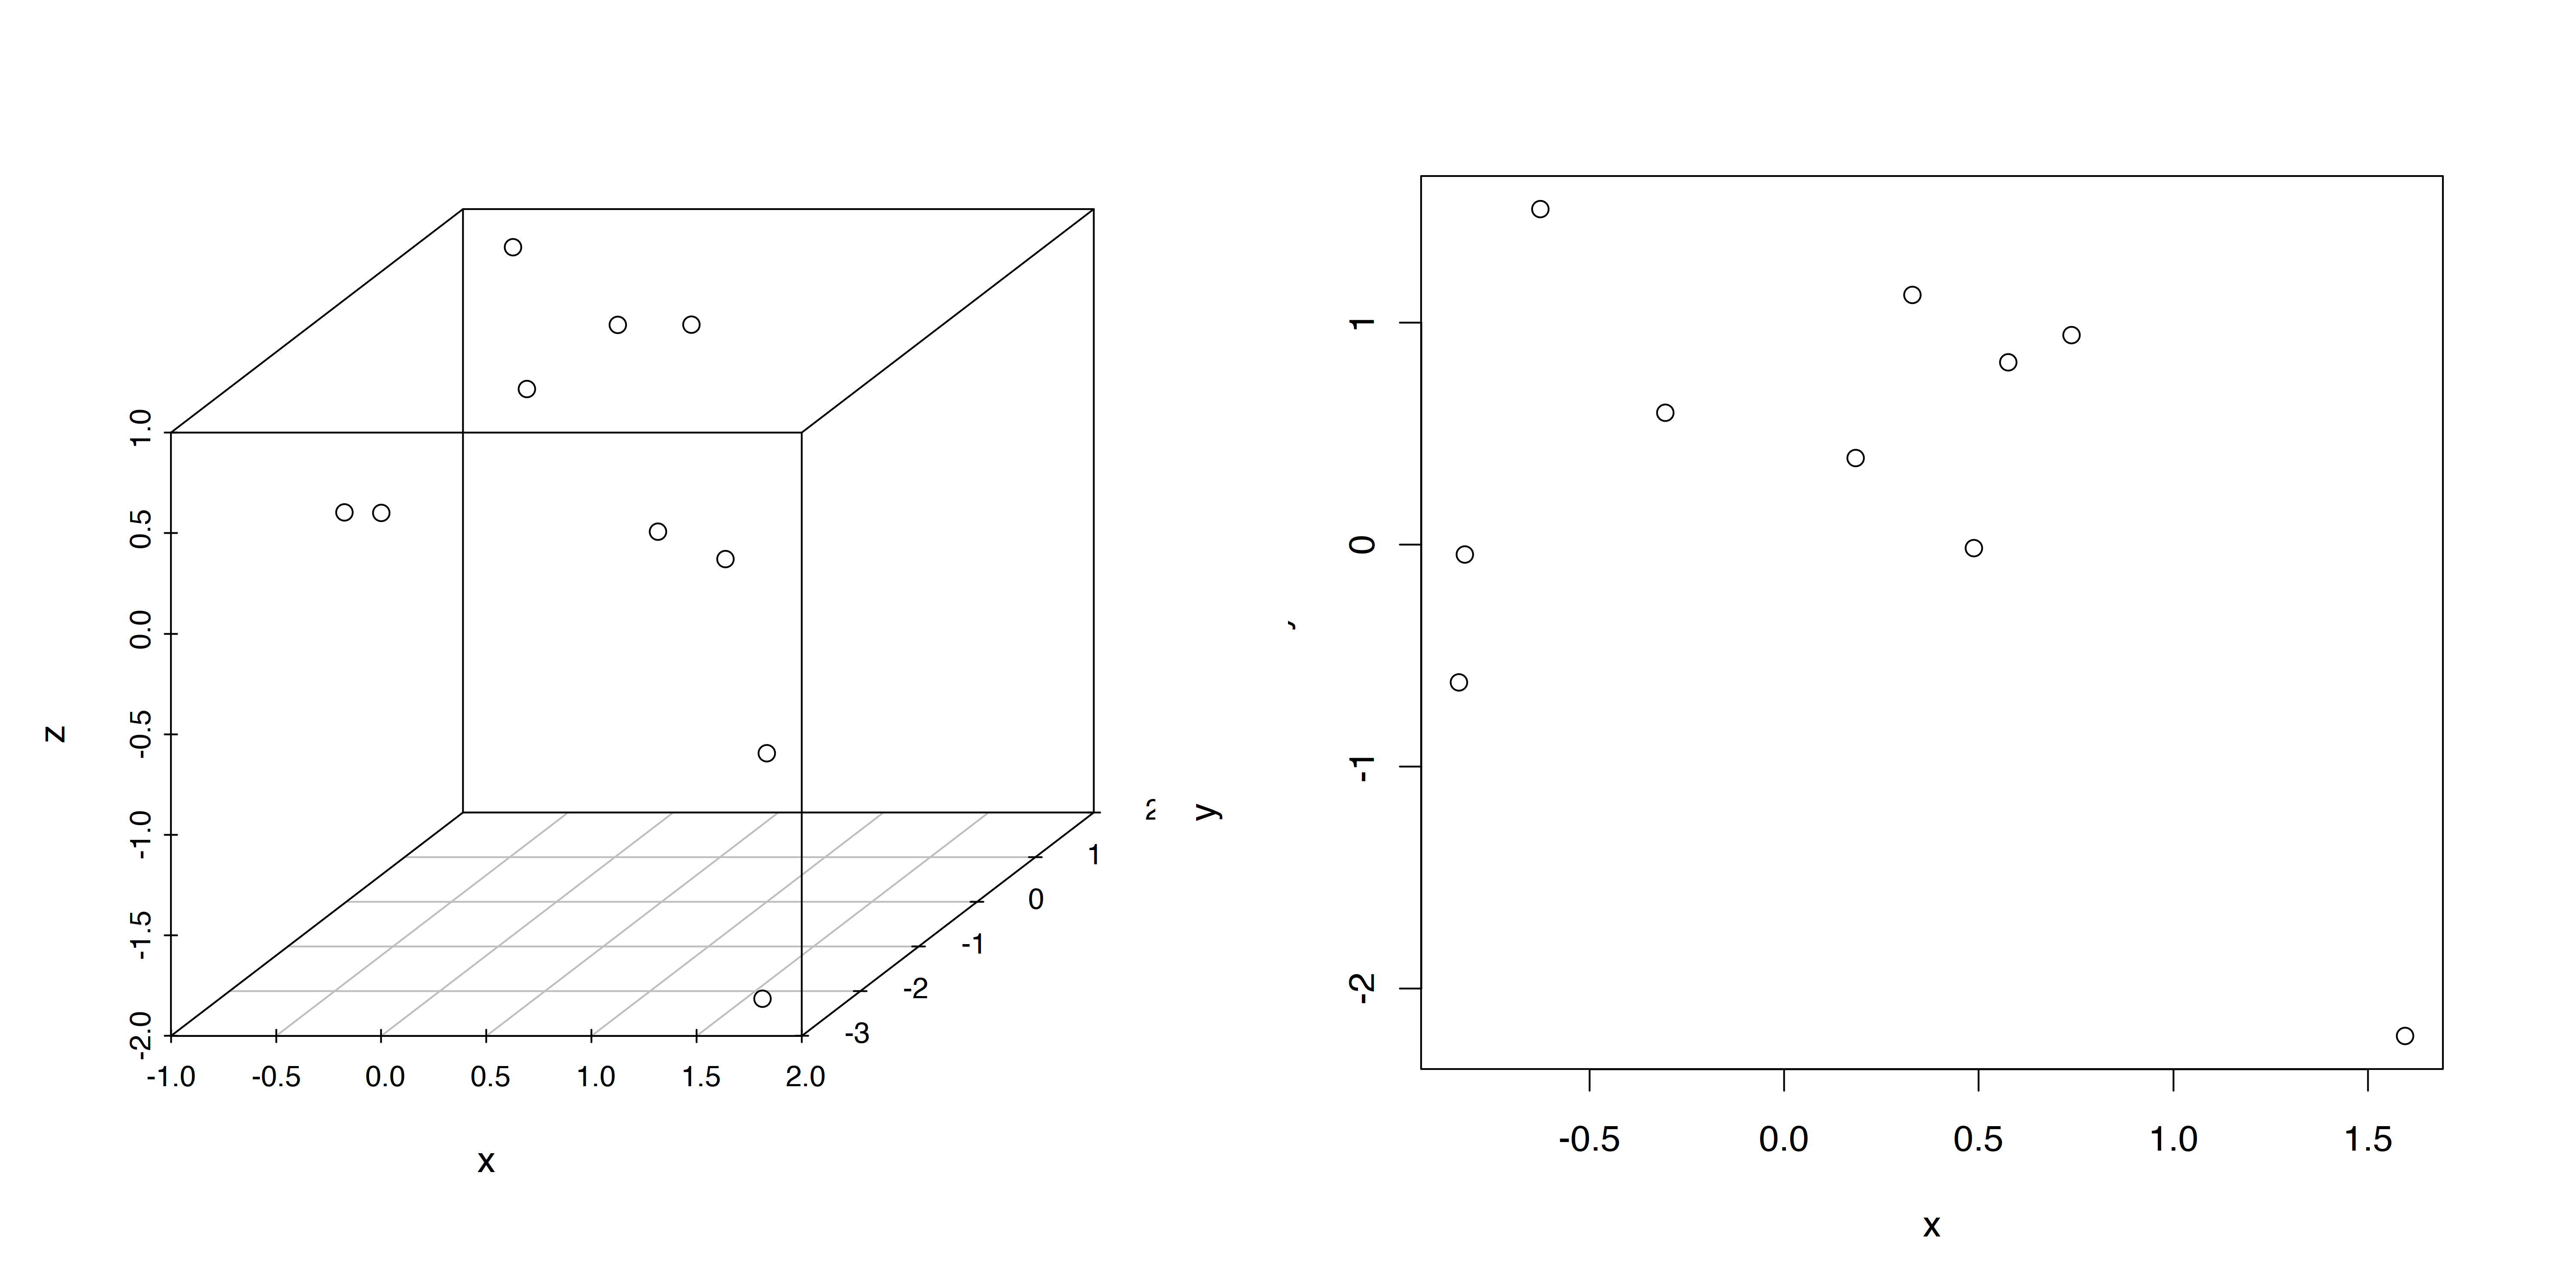
\includegraphics[width=0.8\textwidth]{figures/dimred-1} 

}

\caption{Dimensionalty reduction}\label{fig:dimred}
\end{figure}

Unsupervised learning includes more tasks than just clustering, outlier detection, association rule learning and dimensionality reduction.
For example, archetypal analysis, latent variables, factor analysis, and more.
Unsupervised learning is truly the colorful bird among the modeling mindsets.

\hypertarget{strengths-7}{%
\section{Strengths}\label{strengths-7}}

\begin{itemize}
\tightlist
\item
  Find hidden pattern in the data that modelers using a supervised learning mindset would likely miss.
\item
  The overall mindset is very open in terms of the range of tasks included, how success can be evaluated, and openness to results and new discoveries.
\item
  The openness for discovery can also mean discovering new business opportunities, learning something new, or gaining scientific insights.
\item
  The world is messy. One often has data, and a sense that the data might be potentially insightful. In this case, the unsupervised learning mindset is wonderful because it gives you the ability to just dive in.
\item
  As a more exploratory mindset, unsupervised learning can be a good starting point for further analysis of the data. These further steps can be done with a different mindset.
\item
  Unlike any other mindset, unsupervised machine learning is able to sift through high-dimensional and complex data, partially automatically.
\item
  Unsupervised learning works without a ground truth. This means no effort is required to label data.
\end{itemize}

\hypertarget{limitations-7}{%
\section{Limitations}\label{limitations-7}}

\begin{itemize}
\tightlist
\item
  One of the major limitations is the lack of ground truth, which comes with the difficulty of evaluating the resulting models. As a result, there are many methods with often very different results.\textsuperscript{\protect\hyperlink{ref-hastie2009elements}{23}}
\item
  Unsupervised machine learning is a good approach to the curse of dimensionality, but even so, unsupervised machine learning can suffer greatly. For example, the more features there are, the more meaningless and difficult to interpret the clusters become.
\item
  In order for the modeling results to make sense, to patterns usually need to be interpreted. This is especially true for clustering and association rule learning. This requires expertise and human intervention.
\item
  There is no guarantee that meaningful patterns will be uncovered. And if no patterns are uncovered, there is no guarantee that another unsupervised would have uncovered something interesting.
\end{itemize}

\hypertarget{resources-1}{%
\section{Resources}\label{resources-1}}

\begin{itemize}
\tightlist
\item
  The book Machine learning: a probabilistic perspective by Keven Murphy.\textsuperscript{\protect\hyperlink{ref-murphy2012machine}{24}}
\end{itemize}

\hypertarget{reinforcement-learning}{%
\chapter{Reinforcement Learning}\label{reinforcement-learning}}

\begin{itemize}
\tightlist
\item
  The world is dynamic: The model is about an actor acting in an environment. The actions of the agent are only rewarded at the end.
\item
  Reinforcement learning balances exploration and exploitation,
\item
  A sub-mindset of \protect\hyperlink{machine-learning}{machine learning}.
\end{itemize}

\textbf{This chapter is under construction! Stay tuned.}

\hypertarget{deep-learning}{%
\chapter{Deep Learning}\label{deep-learning}}

\begin{itemize}
\tightlist
\item
  Neural networks based on stacking various layers of neurons.
\item
  World of feature embeddings, transfer learning and foundation models.
\item
  A machine learning mindset, can also be used for \protect\hyperlink{supervised-ml}{supervised learning}.
\end{itemize}

\textbf{This chapter is under construction! Stay tuned.}

\hypertarget{interpretable-ml}{%
\chapter{Interpretable Machine Learning}\label{interpretable-ml}}

\begin{itemize}
\tightlist
\item
  Models are built with a machine learning mindset: The best approximation of the task at hand.
\item
  The model is interpreted with additional tools.
\item
  Often takes an external view of the model: Describing how it behaves instead of analyzing the components.
\item
  A \protect\hyperlink{machine-learning}{machine learning mindset}.
\end{itemize}

\textbf{This chapter is under construction! Stay tuned.}

\hypertarget{design-based-inference}{%
\chapter{Design-based Inference}\label{design-based-inference}}

\begin{itemize}
\tightlist
\item
  Focused on sampling data representatively rather than complex modeling.
\item
  Data population is finite; uncertainty about results is only due to sampling.
\item
  Often combined with \protect\hyperlink{statistical-modeling}{Statistical Modeling}, especially \protect\hyperlink{frequentist-inference}{Frequentist Inference}.
\end{itemize}

\textbf{This chapter is under construction! Stay tuned.}

\hypertarget{references-1}{%
\chapter*{References}\label{references-1}}


\hypertarget{refs}{}
\begin{CSLReferences}{0}{0}
\leavevmode\vadjust pre{\hypertarget{ref-weisberg2012simulation}{}}%
\CSLLeftMargin{1. }
\CSLRightInline{Weisberg M. Simulation and similarity: Using models to understand the world. Oxford University Press; 2012. }

\leavevmode\vadjust pre{\hypertarget{ref-weisberg2007modeler}{}}%
\CSLLeftMargin{2. }
\CSLRightInline{Weisberg M. Who is a modeler? The British journal for the philosophy of science. 2007;58(2):207--33. }

\leavevmode\vadjust pre{\hypertarget{ref-mcelreath2020statistical}{}}%
\CSLLeftMargin{3. }
\CSLRightInline{McElreath R. Statistical rethinking: A bayesian course with examples in r and stan. Chapman; Hall/CRC; 2020. }

\leavevmode\vadjust pre{\hypertarget{ref-kao2001alcohol}{}}%
\CSLLeftMargin{4. }
\CSLRightInline{Kao WL, Puddey IB, Boland LL, Watson RL, Brancati FL. Alcohol consumption and the risk of type 2 diabetes mellitus: Atherosclerosis risk in communities study. American journal of epidemiology. 2001;154(8):748--57. }

\leavevmode\vadjust pre{\hypertarget{ref-ioannidis2005most}{}}%
\CSLLeftMargin{5. }
\CSLRightInline{Ioannidis JP. Why most published research findings are false. PLoS medicine. 2005;2(8):e124. }

\leavevmode\vadjust pre{\hypertarget{ref-perezgonzalez2015fisher}{}}%
\CSLLeftMargin{6. }
\CSLRightInline{Perezgonzalez JD. Fisher, neyman-pearson or NHST? A tutorial for teaching data testing. Frontiers in psychology. 2015;223. }

\leavevmode\vadjust pre{\hypertarget{ref-yang1996catalog}{}}%
\CSLLeftMargin{7. }
\CSLRightInline{Yang R, Berger JO. A catalog of noninformative priors. Institute of Statistics; Decision Sciences, Duke University Durham, NC, USA; 1996. }

\leavevmode\vadjust pre{\hypertarget{ref-blei2017variational}{}}%
\CSLLeftMargin{8. }
\CSLRightInline{Blei DM, Kucukelbir A, McAuliffe JD. Variational inference: A review for statisticians. Journal of the American statistical Association. 2017;112(518):859--77. }

\leavevmode\vadjust pre{\hypertarget{ref-tiao1973some}{}}%
\CSLLeftMargin{9. }
\CSLRightInline{Tiao GC, Box GE. Some comments on {``bayes''} estimators. The American Statistician. 1973;27(1):12--4. }

\leavevmode\vadjust pre{\hypertarget{ref-richard2017statistical}{}}%
\CSLLeftMargin{10. }
\CSLRightInline{Richard R. Statistical evidence: A likelihood paradigm. Routledge; 2017. }

\leavevmode\vadjust pre{\hypertarget{ref-hacking1965logic}{}}%
\CSLLeftMargin{11. }
\CSLRightInline{Hacking I. Logic of statistical inference. 1965; }

\leavevmode\vadjust pre{\hypertarget{ref-gandenberger2016not}{}}%
\CSLLeftMargin{12. }
\CSLRightInline{Gandenberger G. Why i am not a likelihoodist. Ann Arbor, MI: Michigan Publishing, University of Michigan Library; 2016. }

\leavevmode\vadjust pre{\hypertarget{ref-lazer2014parable}{}}%
\CSLLeftMargin{13. }
\CSLRightInline{Lazer D, Kennedy R, King G, Vespignani A. The parable of google flu: Traps in big data analysis. Science. 2014;343(6176):1203--5. }

\leavevmode\vadjust pre{\hypertarget{ref-hernan2010causal}{}}%
\CSLLeftMargin{14. }
\CSLRightInline{Hernán MA, Robins JM. Causal inference. CRC Boca Raton, FL; 2010. }

\leavevmode\vadjust pre{\hypertarget{ref-pearl2012calculus}{}}%
\CSLLeftMargin{15. }
\CSLRightInline{Pearl J. The do-calculus revisited. arXiv preprint arXiv:12104852. 2012; }

\leavevmode\vadjust pre{\hypertarget{ref-pearl2009causal}{}}%
\CSLLeftMargin{16. }
\CSLRightInline{Pearl J. Causal inference in statistics: An overview. Statistics surveys. 2009;3:96--146. }

\leavevmode\vadjust pre{\hypertarget{ref-athey2016recursive}{}}%
\CSLLeftMargin{17. }
\CSLRightInline{Athey S, Imbens G. Recursive partitioning for heterogeneous causal effects. Proceedings of the National Academy of Sciences. 2016;113(27):7353--60. }

\leavevmode\vadjust pre{\hypertarget{ref-hornik1989multilayer}{}}%
\CSLLeftMargin{18. }
\CSLRightInline{Hornik K, Stinchcombe M, White H. Multilayer feedforward networks are universal approximators. Neural networks. 1989;2(5):359--66. }

\leavevmode\vadjust pre{\hypertarget{ref-breiman2001statistical}{}}%
\CSLLeftMargin{19. }
\CSLRightInline{Breiman L. Statistical modeling: The two cultures (with comments and a rejoinder by the author). Statistical science. 2001;16(3):199--231. }

\leavevmode\vadjust pre{\hypertarget{ref-caruana2015intelligible}{}}%
\CSLLeftMargin{20. }
\CSLRightInline{Caruana R, Lou Y, Gehrke J, Koch P, Sturm M, Elhadad N. Intelligible models for healthcare: Predicting pneumonia risk and hospital 30-day readmission. In: Proceedings of the 21th ACM SIGKDD international conference on knowledge discovery and data mining. 2015. p. 1721--30. }

\leavevmode\vadjust pre{\hypertarget{ref-lapuschkin2019unmasking}{}}%
\CSLLeftMargin{21. }
\CSLRightInline{Lapuschkin S, Wäldchen S, Binder A, Montavon G, Samek W, Müller KR. Unmasking clever hans predictors and assessing what machines really learn. Nature communications. 2019;10(1):1--8. }

\leavevmode\vadjust pre{\hypertarget{ref-ribeiro2016should}{}}%
\CSLLeftMargin{22. }
\CSLRightInline{Ribeiro MT, Singh S, Guestrin C. " why should i trust you?" Explaining the predictions of any classifier. In: Proceedings of the 22nd ACM SIGKDD international conference on knowledge discovery and data mining. 2016. p. 1135--44. }

\leavevmode\vadjust pre{\hypertarget{ref-hastie2009elements}{}}%
\CSLLeftMargin{23. }
\CSLRightInline{Hastie T, Tibshirani R, Friedman JH, Friedman JH. The elements of statistical learning: Data mining, inference, and prediction. Vol. 2. Springer; 2009. }

\leavevmode\vadjust pre{\hypertarget{ref-murphy2012machine}{}}%
\CSLLeftMargin{24. }
\CSLRightInline{Murphy KP. Machine learning: A probabilistic perspective. MIT press; 2012. }

\end{CSLReferences}

\printindex
\thispagestyle{empty}


\end{document}
